\chapter{Introducción}

    \section{Motivación}
        
        La Agencia Digital de Andalucía (ADA) presentó en 2021 un plan de inversión para los años 2022-2025 que se centra en varias áreas estratégicas de desarrollo tecnológico, incluyendo la ciberseguridad; esta inversión del Gobierno andaluz no solo impulsará la creación de un Centro de Ciberseguridad que coordinará la Estrategia Andaluza de Ciberseguridad 2022-2025, sino que además, pretende conseguir que revierta en el desarrollo económico de la región, que ya ha empezado a aceptar empresas como Google, que ha instalado su Centro de Excelencia de Ciberseguridad en Málaga.
        
        Bajo el paraguas de este desarrollo tecnológico, el aumento de la demanda de profesionales en este campo ha despertado un gran interés en los estudiantes por aprender sobre la ciberseguridad.
        
        Sin embargo, muchos de ellos se enfrentan a la dificultad de encontrar recursos educativos completos y accesibles debido a las restricciones que imponen algunas plataformas de entrenamiento, donde los recursos que ofrecen tienen barreras que dificultan el acceso a la formación, incluyendo la necesidad de suscripciones para acceder al contenido completo.
        
        Esto puede desmotivar a los estudiantes y reducir su capacidad para aprender y desarrollar habilidades en el campo de la ciberseguridad.
    
    
    \section{Objetivos}
        \label{sec:objetivos}
    
        Se busca desarrollar de una plataforma web que sea ligera, gratuita, \textit{open-source} y fácilmente extensible, con el objetivo principal de simplificar la introducción de futuros estudiantes en el sector de la ciberseguridad, con un enfoque específico en el pentesting.
        
        La plataforma proporcionará información documentada y sintetizada junto con entornos de prueba virtualizados para facilitar el aprendizaje mediante la experimentación.
        
        A diferencia de otras plataformas como Hack The Box y similares, el enfoque de esta plataforma no estará en la resolución de retos, como serían las pruebas de tipo CTF más habituales en el sector, sino en guiar e instruir a los usuarios de la plataforma sobre distintos conceptos y técnicas de pentesting, proporcionando entornos virtuales diseñados específicamente para experimentar y poner en práctica conceptos concretos.
        
        Esta herramienta brindará a los usuarios una experiencia educativa gratuita y accesible en ciberseguridad, permitiéndoles aprender y desarrollar habilidades prácticas de manera efectiva y en línea con las necesidades del mercado.
    
    
    \section{Metodología}
    
        Se ha empleado un \textbf{desarrollo incremental} para la elaboración del proyecto: se partió de una base a la que se añadieron sucesivas mejoras sin que estas perjudicaran al resto del proyecto desarrollado hasta ese momento.

        \begin{figure}[htbp]
            \centering

            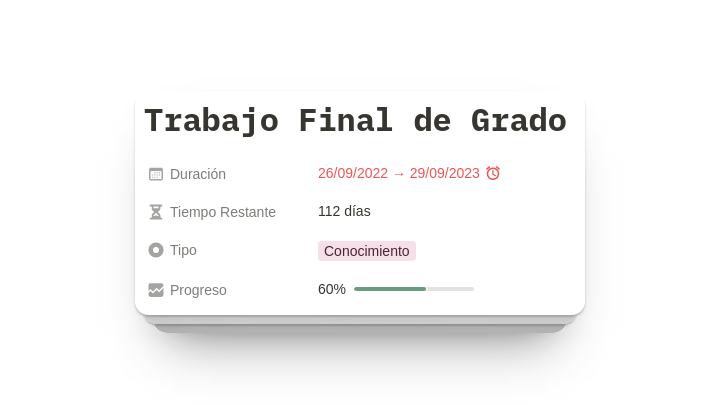
\includegraphics[width=0.75\textwidth]{images/Capturas/Notion resumen.png}
            \caption{Resumen del estado del proyecto en Notion al momento de la captura}
            \label{fig:notion-resumen}
        \end{figure}

        Se ha utilizado la herramienta \textbf{Notion} para llevar a cabo este proyecto, una aplicación que permite la creación de notas -llamadas páginas- cuyo contenido puede ser variado: texto, imágenes, tablas, listas, archivos, enlaces... y que además, permite la creación de bases de datos que pueden ser utilizadas para crear tablones Kanban, diagramas de Gantt, y otros tipos de vistas dinámicas.

        Notion también cuenta con otra funcionalidad recientemente añadida: la integración con GitHub \cite{github}. Esto permite añadir a cualquier página de Notion una base de datos generada a partir del estado de un repositorio remoto -\textit{Issues}, \textit{Projects} y \textit{Pull Requests}-, permitiendo además la manipulación y la actualización del contenido en ambas direcciones, todo sincronizado a tiempo real. 

        El proceso que se ha seguido para el desarrollo del proyecto ha sido definir tareas en Notion y descomponerlas en tareas más simples, atómicas y tratables, clasificadas en función de su propósito: componer la memoria, desarrollar la plataforma web o crear entornos de pruebas virtualizados. Por otra parte, se han asignado dependencias entre las tareas, por lo que en la mayoría de ocasiones resultaba intuitivo y visual establecer el orden que debían seguir dichas tareas.

        \newpage

        \begin{figure}[!htbp]
            \centering

            \begin{subfigure}[!htbp]{\textwidth}
                \centering

                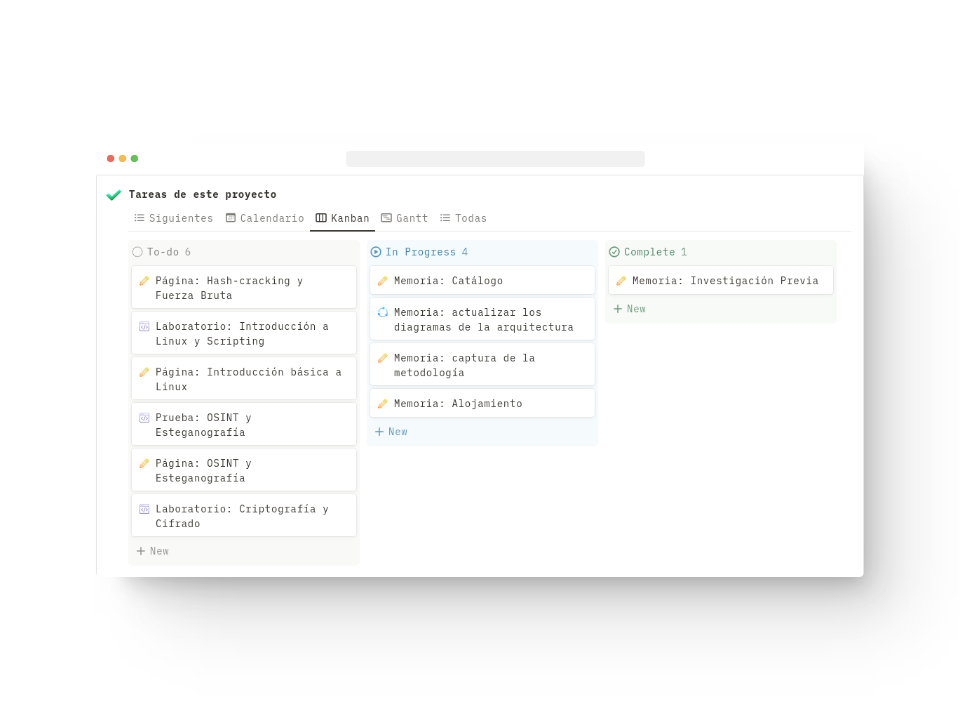
\includegraphics[width=0.8\textwidth]{images/Capturas/Notion Kanban.png}
                \caption{Vista de Kanban}
            \end{subfigure}
            
            \begin{subfigure}[!htbp]{\textwidth}
                \centering

                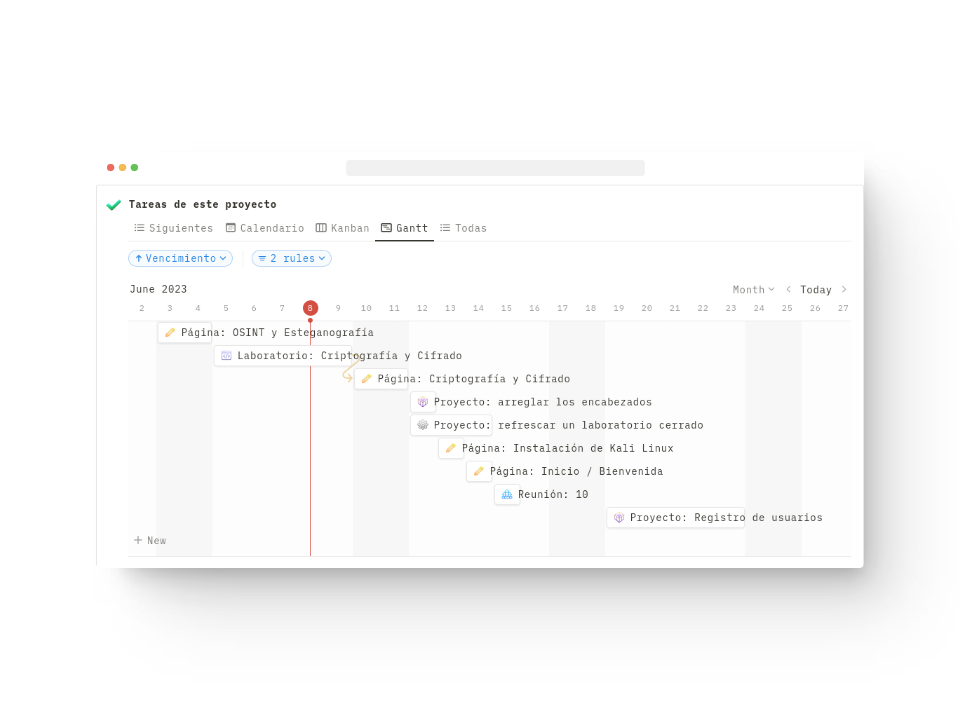
\includegraphics[width=0.8\textwidth]{images/Capturas/Notion Gantt.png}
                \caption{Vista de Gantt}
            \end{subfigure}
            
            \caption{Gestión de tareas del proyecto en una base de datos de Notion}
            \label{fig:notion-vistas}
        \end{figure}
        
        El desarrollo se ha llevado a cabo utilizando, principalmente, las vistas de los sistemas: Kanban, con las tareas clasificadas en función de su estado; y Gantt, con las tareas clasificadas y ordenadas en función de sus dependencias. No obstante, también se han utilizado las vistas de Lista para visualizar las tareas de una forma más compacta y ordenada, y de Calendario para visualizar las tareas en función de su fecha de finalización.
        
        \newpage
    
    \section{Estructura global del proyecto}
        \label{sec:estructura-global}
        
        El proyecto se divide en tres pilares principales: la creación de una plataforma web, la investigación y selección de conceptos de pentesting y la virtualización de los entornos de prueba, resultando en el objetivo de este proyecto de trabajo de fin de grado, una plataforma web que proporcionará información sobre técnicas de pentesting y ofrecerá acceso a pruebas virtualizadas en forma de laboratorios. 
        
        \begin{figure}[h]
            \centering
            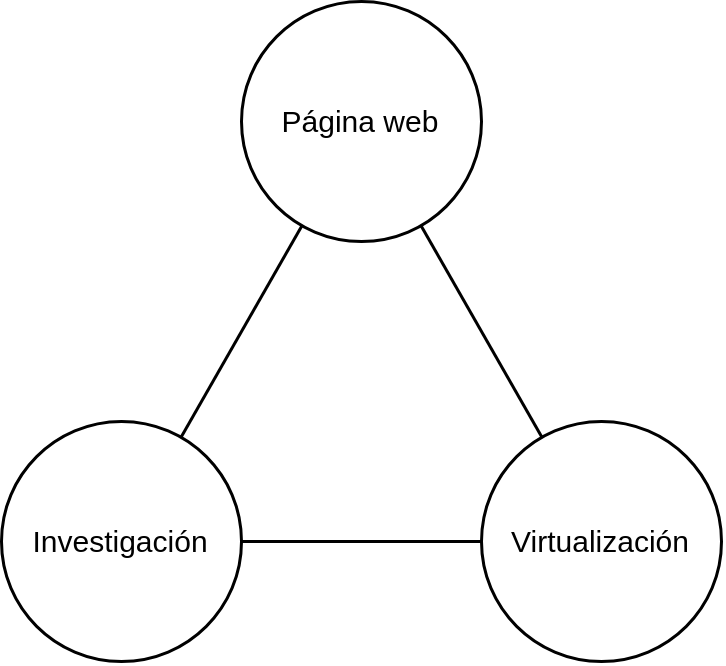
\includegraphics[scale=0.30]{images/Diagramas/Estructura global.png}
            \caption{Pilares fundamentales del proyecto}
            \label{fig:estructura-global}
        \end{figure}
            
        \subsection{Página web}
        
            La primera toma de contacto del usuario con la plataforma, la página web será la interfaz de usuario para acceder a los laboratorios y contenidos relacionados con la ciberseguridad.
            
            Respecto a su construcción, se han considerado dos opciones: programarla desde cero o utilizar un CMS (Sistema de Gestión de Contenidos); para la primera opción, se optaría por el uso del framework Astro, que permite crear sitios web rápidamente, además de proporcionar un amplio conjunto de herramientas para su personalización; por otro lado, se ha considerado el uso de WordPress, uno de los CMS más utilizados en el mundo y que cuenta con una amplia variedad de plantillas disponibles, lo que facilitaría el diseño de la interfaz.

            También se tuvieron en cuenta distintos constructores de páginas webs como Cargo Collective o Square Space.

            Finalmente, se decidió usar WordPress por su sencillez y su biblioteca de plugins, que permitiría integrar diferentes funcionalidades extra en lugar de programarlas manualmente como podría haber ocurrido con el uso de un framework.
                
            \subsubsection{Alojamiento}
            
                Respecto al alojamiento, se han considerado varias opciones, tales como GitHub Pages, Vercel, OVHcloud o Heroku.
                
                Sin embargo, al tratarse de una prueba de concepto, se ha decidido elaborar la infraestructura de forma local, lo que permitirá un mayor control y flexibilidad en el desarrollo, dando lugar a mejoras en futuras líneas de trabajo \ref{sec:futuras-lineas-trabajo}.

                En cuanto a la base de datos, se ha decidido utilizar MySQL por ser una opción muy utilizada, fácil de configurar y ser nativamente compatible con WordPress. La base de datos tendrá la menor cantidad de tablas posibles, almacenando únicamente la información necesaria sobre los usuarios registrados y sobre los laboratorios.
            
        \subsection{Investigación}
        
            Se centrará en recopilar y seleccionar diferentes conceptos y técnicas relacionados con el pentesting. Este apartado se verá mejor reflejado en la sección Catálogo \ref{sec:catalogo}.
        
        \subsection{Virtualización}

            La virtualización es una parte integral del proyecto, ya que permite la creación de varios laboratorios de prueba donde los usuarios aplicarán los conocimientos adquiridos en la plataforma; concretamente, se consideraron contenedores de Docker y máquinas virtuales para crear estos laboratorios.
            
            Elegir Docker como plataforma de contenedores es una buena opción porque ofrece una gestión de recursos eficiente y una generación de imágenes sencilla; por otro lado, Vagrant Cloud es una buena opción para crear máquinas virtuales, ya que ofrece una amplia gama de imágenes preconfiguradas y un entorno de desarrollo fácil de usar.
            
            Se pueden utilizar diversas herramientas para gestionar los contenedores, en función de las necesidades específicas de cada laboratorio; por ejemplo, Kubernetes es una buena herramienta para la gestión de contenedores a gran escala (clústers de contenedores). Además, Docker Compose es una opción conveniente para configurar y ejecutar aplicaciones de contenedores múltiples.
            
            Por otro lado, también se consideraron plataformas que brindan servicios de almacenamiento y distribución de imágenes, como DockerHub para imágenes de contenedores de Docker y Vagrant Cloud para máquinas virtuales preconfiguradas. Estas dos plataformas brindan enlaces de descargas con las que un usuario puede acceder a recursos previamente montados por su autor.

            \newpage

            
    \section{Tecnologías}
    
        Las siguientes tecnologías y herramientas se emplearon en el desarrollo del proyecto:
        
        \subsection{GitHub}
        
            GitHub es una plataforma de desarrollo colaborativo de software que ofrece alojamiento de código fuente, seguimiento de problemas y herramientas de colaboración para proyectos de programación.
            
            Esta plataforma es muy popular en la comunidad de desarrolladores, ya que les permite compartir su trabajo con otros usuarios, pudiendo ser clonado, modificado y actualizado por otros desarrolladores, permitiendo la colaboración y el intercambio de conocimientos; o mantenerlo privado para uso personal o empresarial.
            
            Además del alojamiento de código fuente, GitHub también ofrece herramientas de seguimiento de problemas, donde los desarrolladores pueden reportar y resolver errores, solicitar nuevas características y discutir mejoras en el software. Esto facilita la comunicación y la colaboración entre los usuarios, además de mejorar la calidad del software desarrollado.
            
            
        \subsection{WordPress}
            
            WordPress \cite{wordpress} es una plataforma de código abierto para la creación y gestión de sitios web que fue publicada en 2003 y desde entonces, se ha convertido en una de las plataformas más populares y utilizadas en todo el mundo, siendo especialmente popular para la creación de blogs, aunque también es utilizada para sitios web corporativos, tiendas en línea, portafolios, entre otros. 
            
            WordPress es utilizado por muchos grandes sitios web y empresas, como el blog de noticias TIME \cite{time-web} y el sitio web de la BBC America \cite{bbc-america-web}. También es utilizado por miles de bloggers y pequeñas empresas en todo el mundo debido a su facilidad de uso y capacidad de personalización.

            Una de las principales ventajas de WordPress es que es muy fácil de usar y no se requiere experiencia técnica previa para comenzar a utilizarlo. Otra ventaja de WordPress es su personalización gracias a la gran cantidad de temas y complementos (plugins) disponibles. Estos complementos permiten añadir nuevas funcionalidades a un sitio web, como formularios de contacto, galerías de imágenes, integración con redes sociales... evitando la necesidad de programar dichas funcionalidades de forma manual.
            
            Por otra parte, WordPress es muy \textit{SEO-friendly}, incluyendo características que ayudan a mejorar el posicionamiento en los motores de búsqueda, como la capacidad de editar títulos, descripciones y etiquetas de metadatos, así como la posibilidad de utilizar herramientas de optimización de motores de búsqueda (SEO).
            
            \newpage

            
        \subsection{Docker}
            \label{sec:docker}
        
            Docker es una plataforma de software que permite crear, implementar y administrar aplicaciones en contenedores, siendo un contenedor un entorno aislado y seguro que recoge una aplicación y todas sus dependencias, lo que permite que se ejecute sin problemas en cualquier entorno informático, independientemente de las diferencias entre los sistemas operativos o las configuraciones de hardware.
            
            \begin{figure}[h]
                \centering
                
                \begin{subfigure}[h]{\textwidth}
                    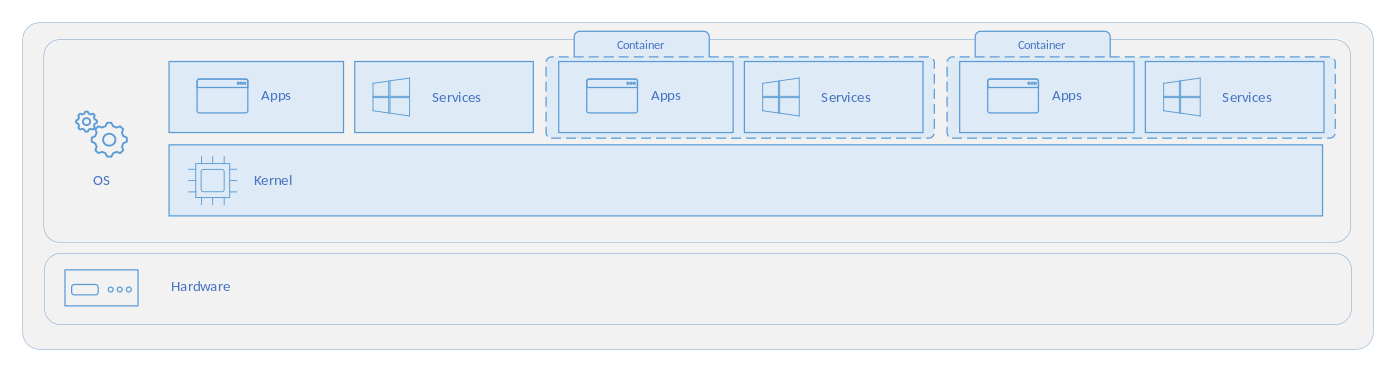
\includegraphics[width=\textwidth]{images/Diagramas/Esquema de Contenedores.png}
                    \caption{Arquitectura de los contenedores}
                    \label{fig:arquitectura-contenedores}
                \end{subfigure}
                
                \begin{subfigure}[h]{\textwidth}
                    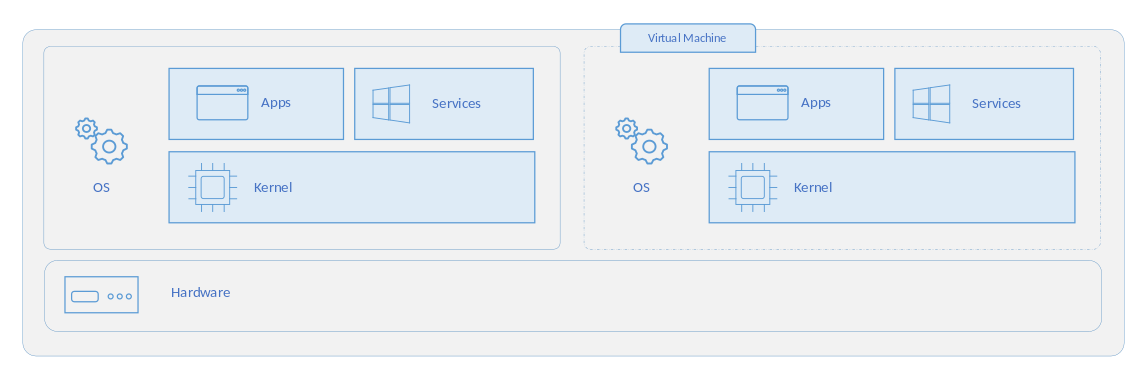
\includegraphics[width=\textwidth]{images/Diagramas/Esquema de MVs.png}
                    \caption{Arquitectura de las máquinas virtuales}
                    \label{fig:arquitectura-maquinasvirtuales}
                \end{subfigure}
                
                \caption{Diferencias entre contenedores y las máquinas virtuales}
                \label{fig:contenedores-vs-maquinasvirtuales}
            \end{figure}
            
            Docker funciona con imágenes, que son plantillas o modelos que contienen todos los componentes necesarios para ejecutar una aplicación en un contenedor, incluidos el código fuente, las librerías, los archivos de configuración y las dependencias del sistema. Estas imágenes pueden ser descargadas desde un registro centralizado llamado Docker Hub o construirse localmente por los desarrolladores.
            
            Una vez obtenida una imagen, puede usarse Docker para crear un contenedor a partir de ella, lo que implica crear una instancia de aplicación y, por tanto, el entorno en el que se ejecuta; los contenedores de Docker se pueden transferir fácilmente entre diferentes sistemas y entornos, lo que facilita la implementación y el escalado de aplicaciones. Además, Docker proporciona herramientas de administración de contenedores, como la capacidad de iniciar, detener, reiniciar y eliminar contenedores, así como la capacidad de monitorear su uso y rendimiento.
            
            \newpage


        \subsection{LAMP}

            Este es un acrónimo que se utiliza comúnmente en el mundo de los servidores para describir un conjunto de tecnologías de código abierto que se utilizan para construir y ejecutar aplicaciones web dinámicas.

            \begin{table}[!htbp]
                  \centering
                  
                  \begin{tabular}{|>{\centering\arraybackslash}m{3cm}|>{\centering\arraybackslash}m{3cm}|>{\centering\arraybackslash}m{8cm}|}
                        \hline
                        \textbf{Componente} & \textbf{Tipo} & \textbf{Descripción} \\
                        \hline
                        \hline
                        \textbf{Linux} & Sistema Operativo & Utilizado ampliamente en servidores web debido a su fiabilidad, seguridad y flexibilidad. \\
                        \hline
                        \textbf{Apache} & Servidor Web & Alojamiento de sitios web y aplicaciones web. \\
                        \hline
                        \textbf{MySQL} & RDBMS & Almacenamiento y recuperación de información para aplicaciones web. \\
                        \hline
                        \textbf{PHP} & Lenguaje de Programación & Creación de sitios web y aplicaciones web dinámicas. Procesa la lógica de la aplicación en el servidor. \\
                        \hline
                  \end{tabular}

                  \caption{Componentes habituales de la pila de software LAMP}
                  \label{table:lamp}
            \end{table}
            
            Algunas veces, la P de LAMP es sustituida por Perl o Python.                  

            \cleardoublepage

    
     
\chapter{Estado del arte}
    \label{cap:estado-arte}

    Actualmente existen diversas plataformas web de entrenamiento en ciberseguridad que ofrecen laboratorios y desafíos para mejorar las habilidades de seguridad ofensiva y defensiva de los usuarios; dichas plataformas han experimentado un crecimiento en popularidad en los últimos años debido a la creciente demanda de profesionales en el campo de la seguridad informática y a la necesidad de mejorar las habilidades tanto de los estudiantes como de los profesionales en el campo.
    
    Estas plataformas varían en su enfoque y contenido, desde laboratorios que simulan entornos de la vida real hasta desafíos de explotación de vulnerabilidades, así como eventos de naturaleza más lúdica y competitiva como los retos de capturar la bandera, también conocidos como CTFs (\textit{Capture The Flag}).
    
    Algunas de estas plataformas han sido utilizadas en la educación, ya que permiten a los usuarios practicar y aplicar conceptos teóricos de seguridad informática en un entorno práctico; y también pueden ser útiles para empresas y organizaciones, ya sea para evaluar las habilidades de seguridad de los empleados o para mejorar la seguridad de sus sistemas.
    
    Respecto al futuro, se espera que continúen creciendo en popularidad y que aumente la variedad de laboratorios y desafíos que ofrecen, siendo muy probable que se produzca una mayor integración con otras tecnologías de inteligencia artificial, quizás dando lugar a una mejora en la calidad de esos desafíos y laboratorios mencionados, para que proporcionen una experiencia de usuario más personalizada.
    
    A continuación se presenta una breve descripción de algunas de las plataformas más populares actualmente, donde se muestran sus similitudes y sus diferencias:
    
    \newpage
    
    
    \section{Hack The Box}
    
        Plataforma web de entrenamiento que ofrece más de 200 desafíos y laboratorios de amplia variedad, diseñados para mejorar las habilidades de seguridad ofensiva y defensiva de los usuarios. Hack The Box se ha vuelto \textbf{la plataforma más popular} en la comunidad de seguridad informática debido a su \textbf{enfoque en la calidad de los desafíos y laboratorios} y su \textbf{comunidad activa de usuarios}.
        
        Sus retos abarcan desde desafíos básicos de hacking hasta laboratorios avanzados, y también ofrece una función llamada \textit{Boxes} diseñada para simular entornos de la vida real, como redes empresariales, que contienen múltiples vulnerabilidades que los usuarios pueden explotar para ganar acceso a sistemas y obtener información confidencial.
        
        \begin{figure}[h]
            \centering
            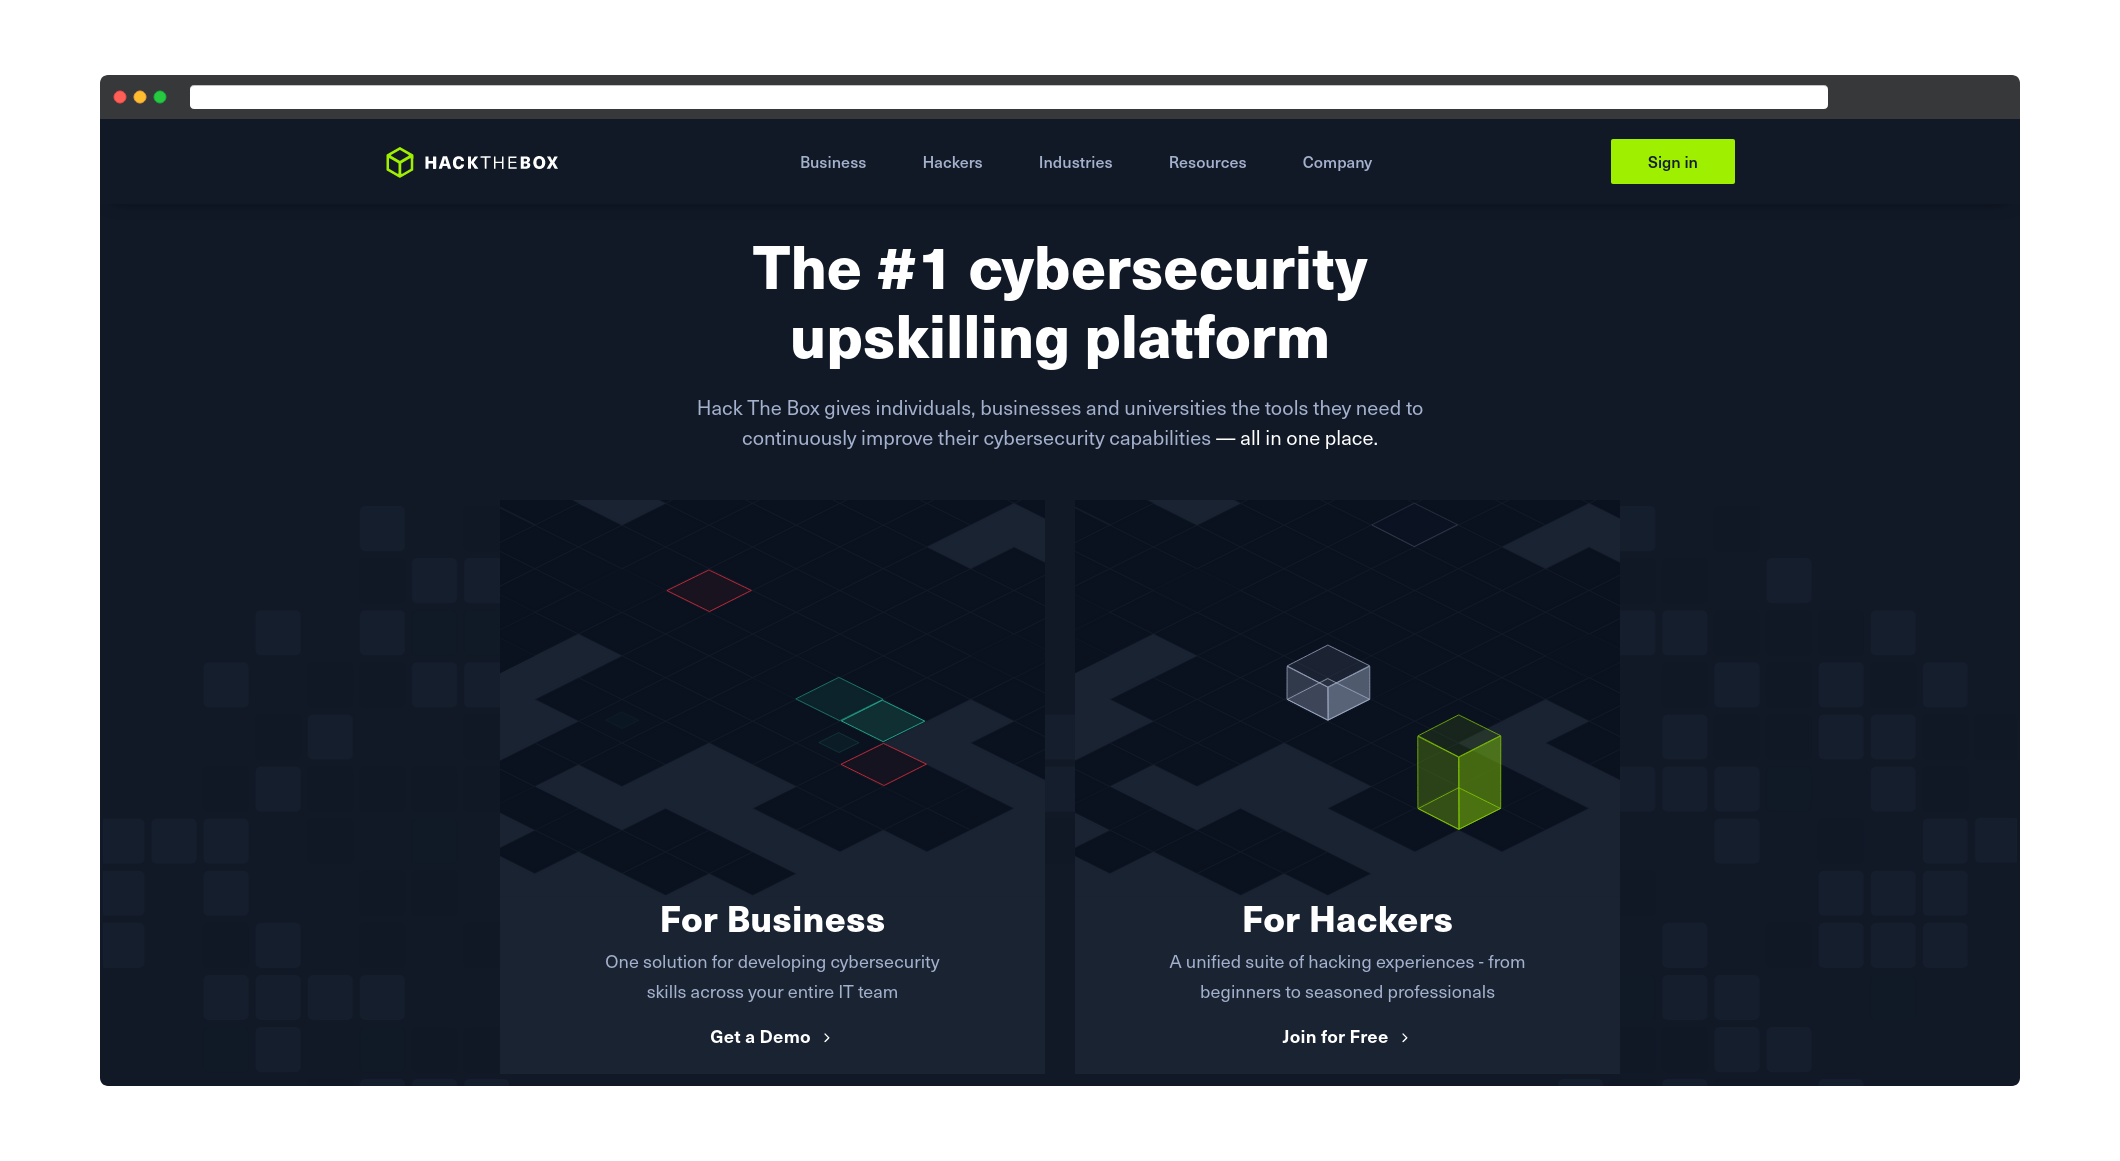
\includegraphics[width=\textwidth]{images/Capturas/Web de HTB.png}
            \caption{Web de Hack The Box}
            \label{fig:HTB-web}
        \end{figure}
        
        Una de las características más interesantes de esta plataforma es su enfoque en el hacking ético, ya que se fomenta una cultura de hacking responsable y legal y requiere que los usuarios acepten un código de conducta antes de unirse. Los usuarios también son alentados a informar sobre cualquier vulnerabilidad que encuentren en la plataforma.
        
        Hack the Box ofrece diferentes \textbf{planes de suscripción} para los usuarios interesados en acceder a su contenido:
        
        \begin{itemize}
            \item \textbf{Plan gratuito}: acceso limitado a una selección de desafíos y laboratorios, pero no incluye acceso a los \textit{boxes}.
        
            \item \textbf{Plan VIP}: acceso completo a la plataforma (todos los laboratorios, desafíos y \textit{boxes} disponibles).
        
            \item \textbf{Planes empresariales}: personalizados para empresas y organizaciones que deseen utilizar la plataforma para la formación y evaluación de sus empleados en seguridad informática.
        \end{itemize}
        
        \newpage

    
    \subsection{HTB Academy}
    
        Esta es una iniciativa de Hack The Box que también ofrece formación, pero al contrario que Hack The Box, centrada en la práctica y el desafío en tiempo real, HTB Academy \textbf{se enfoca en la enseñanza práctica de habilidades a través de cursos y laboratorios}.
        
        \begin{figure}[h]
            \centering
            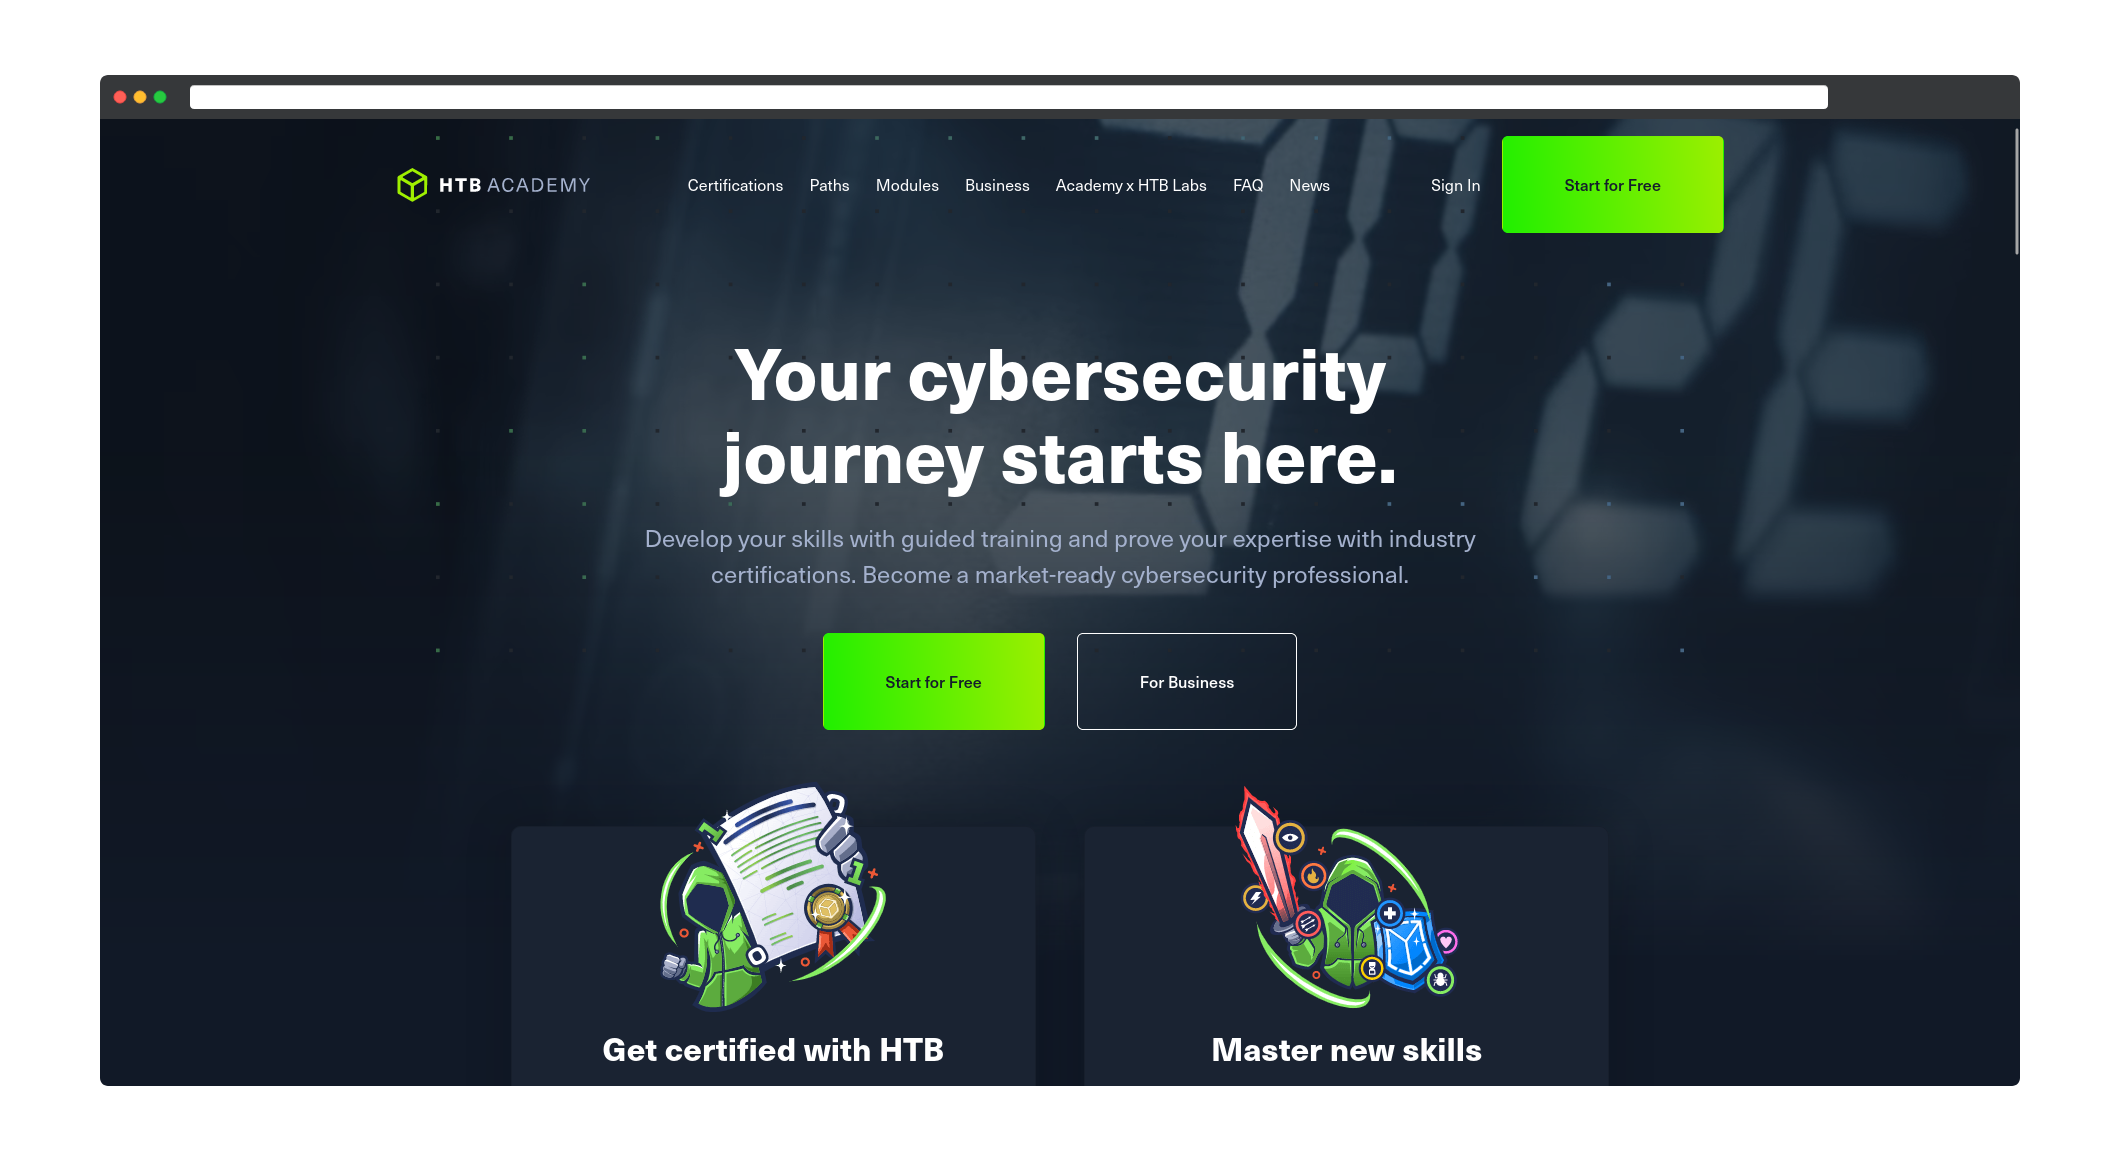
\includegraphics[width=\textwidth]{images/Capturas/Web de HTB Academy.png}
            \caption{Web de HTB Academy}
            \label{fig:HTB-Academy-web}
        \end{figure}
        
        Los cursos están diseñados para ser prácticos, con una orientación en la experimentación activa que permite a los usuarios adquirir habilidades en la práctica, y no solo a través de la teoría; cubren una amplia gama de temas, desde los fundamentos de la seguridad informática hasta temas avanzados como el análisis de malware, el hacking web y la ingeniería inversa, ya que están diseñados para ser accesibles desde principiantes hasta expertos en el sector.
        
        Esta plataforma cuenta con los mismos tipos de \textbf{planes de suscripción} que Hack The Box: gratuito, VIP y empresarial; aunque es importante destacar que tanto Hack The Box como HTB Academy son servicios diferentes, por lo que \textbf{los planes de ambas plataformas son completamente independientes entre sí}.
        
        \newpage
    
    
    \section{TryHackMe}
    
        Plataforma de aprendizaje de ciberseguridad basada en la experimentación activa, que proporciona una variedad de entornos de laboratorio virtuales y desafíos prácticos para ayudar a los usuarios a aprender y mejorar sus habilidades en seguridad informática; su contenido se encuentra organizado en \textbf{diferentes rutas de aprendizaje} que permiten a los usuarios desarrollar su conocimiento de forma estructurada.
        
        \begin{figure}[h]
            \centering
            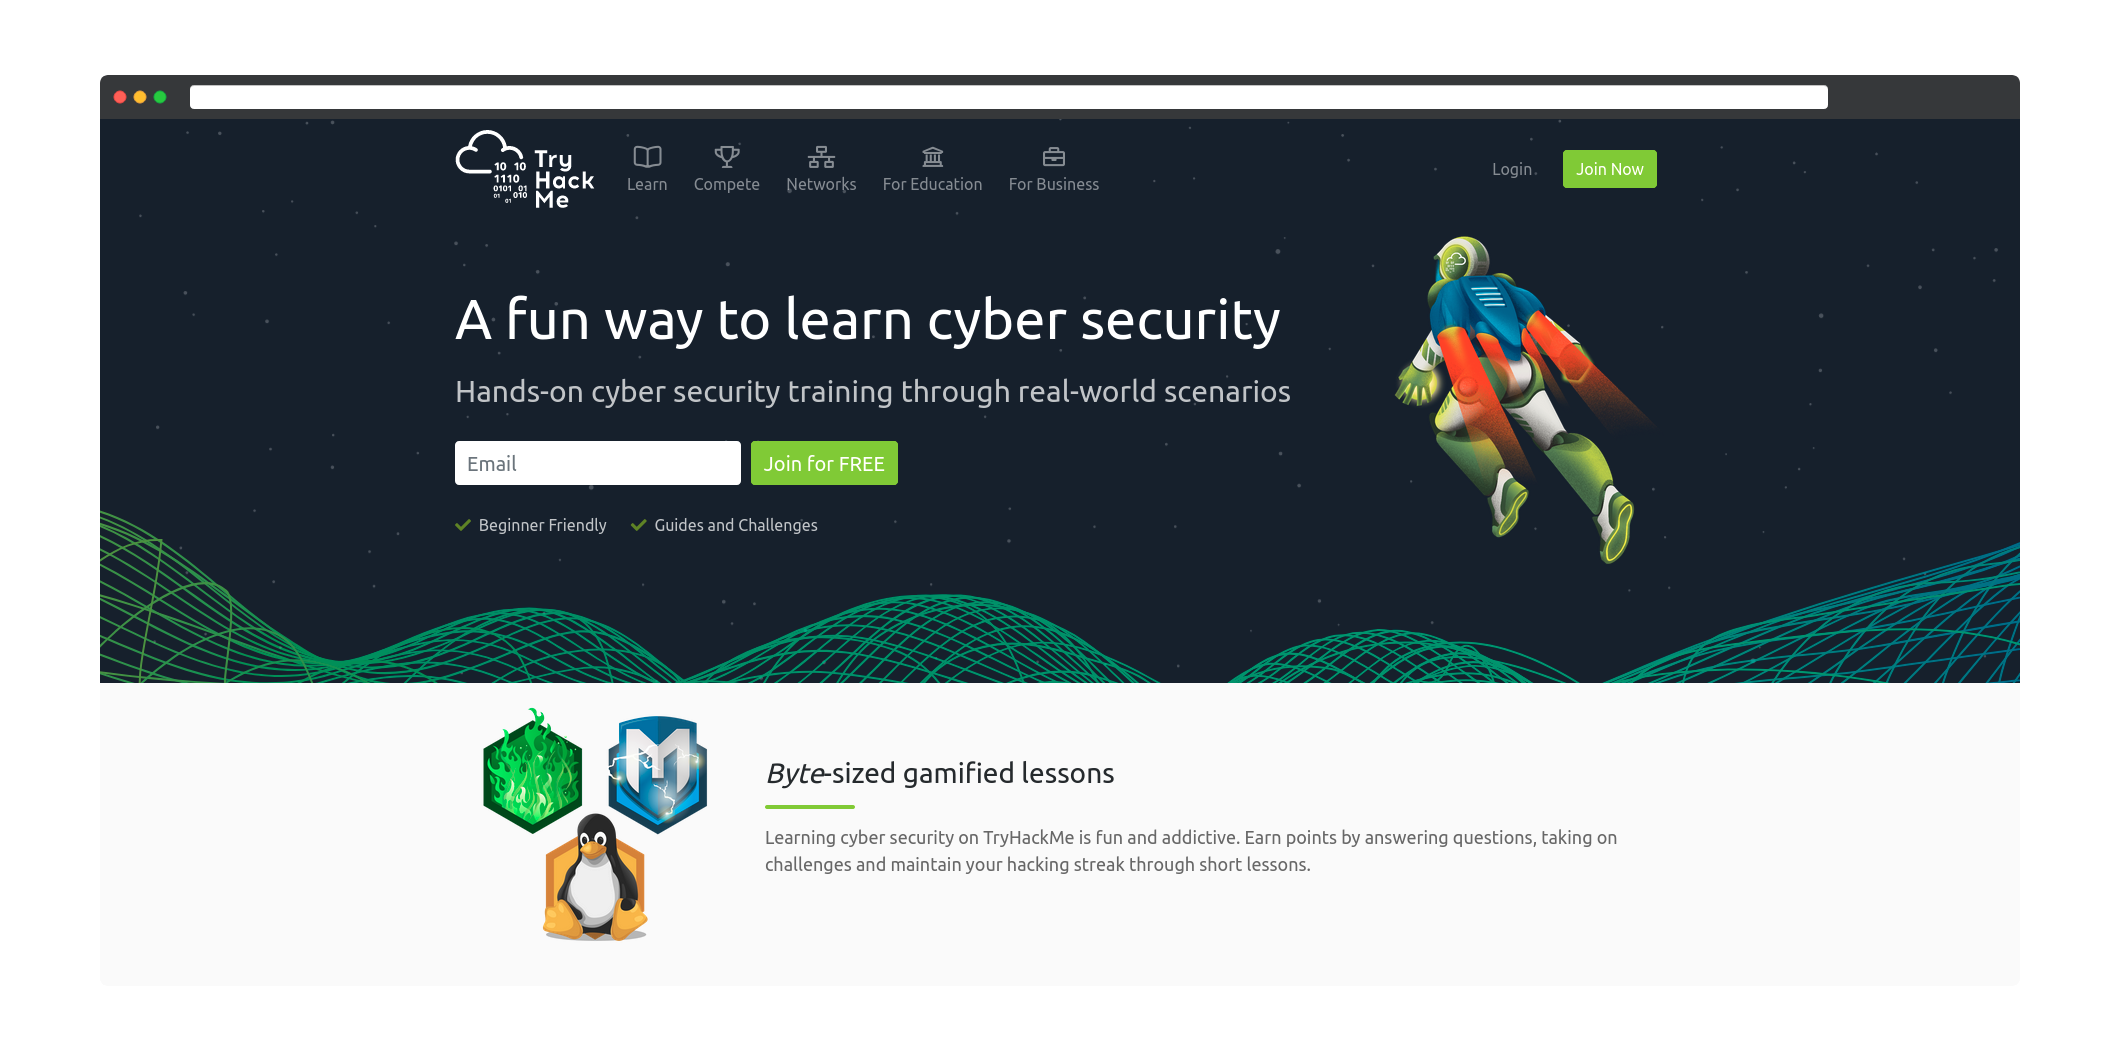
\includegraphics[width=\textwidth]{images/Capturas/Web de THM.png}
            \caption{Web de TryHackMe}
            \label{fig:THM-web}
        \end{figure}
        
        La plataforma también cuenta con una comunidad activa y una función de \textit{gamificación} que proporciona una experiencia de aprendizaje más interactiva y entretenida, permitiendo que los usuarios puedan competir entre ellos, ganando puntos y recompensas por completar desafíos y resolver problemas de seguridad.
        
        TryHackMe ofrece diferentes \textbf{planes de suscripción} para los usuarios interesados:
        
        \begin{itemize}
            \item \textbf{Plan gratuito}: acceso limitado a una selección de desafíos y laboratorios.
        
            \item \textbf{Plan premium}: acceso completo a la plataforma (todos los laboratorios y desafíos).
        
            \item \textbf{Planes empresariales}: personalizados para empresas y organizaciones que deseen utilizar la plataforma para la formación y evaluación de sus empleados en seguridad informática.
        \end{itemize}
        
        \newpage
    
    
    \section{VulnHub}
    
        Plataforma de laboratorios que proporciona una gran cantidad de \textbf{máquinas virtuales vulnerables que los usuarios pueden descargar} y configurar en sus propios entornos de laboratorio para luego explotar sus vulnerabilidades; cada máquina virtual cuenta con descripción detallada de su objetivo y una guía paso a paso para ayudar a los usuarios en su proceso de aprendizaje.
        
        \begin{figure}[h]
            \centering
            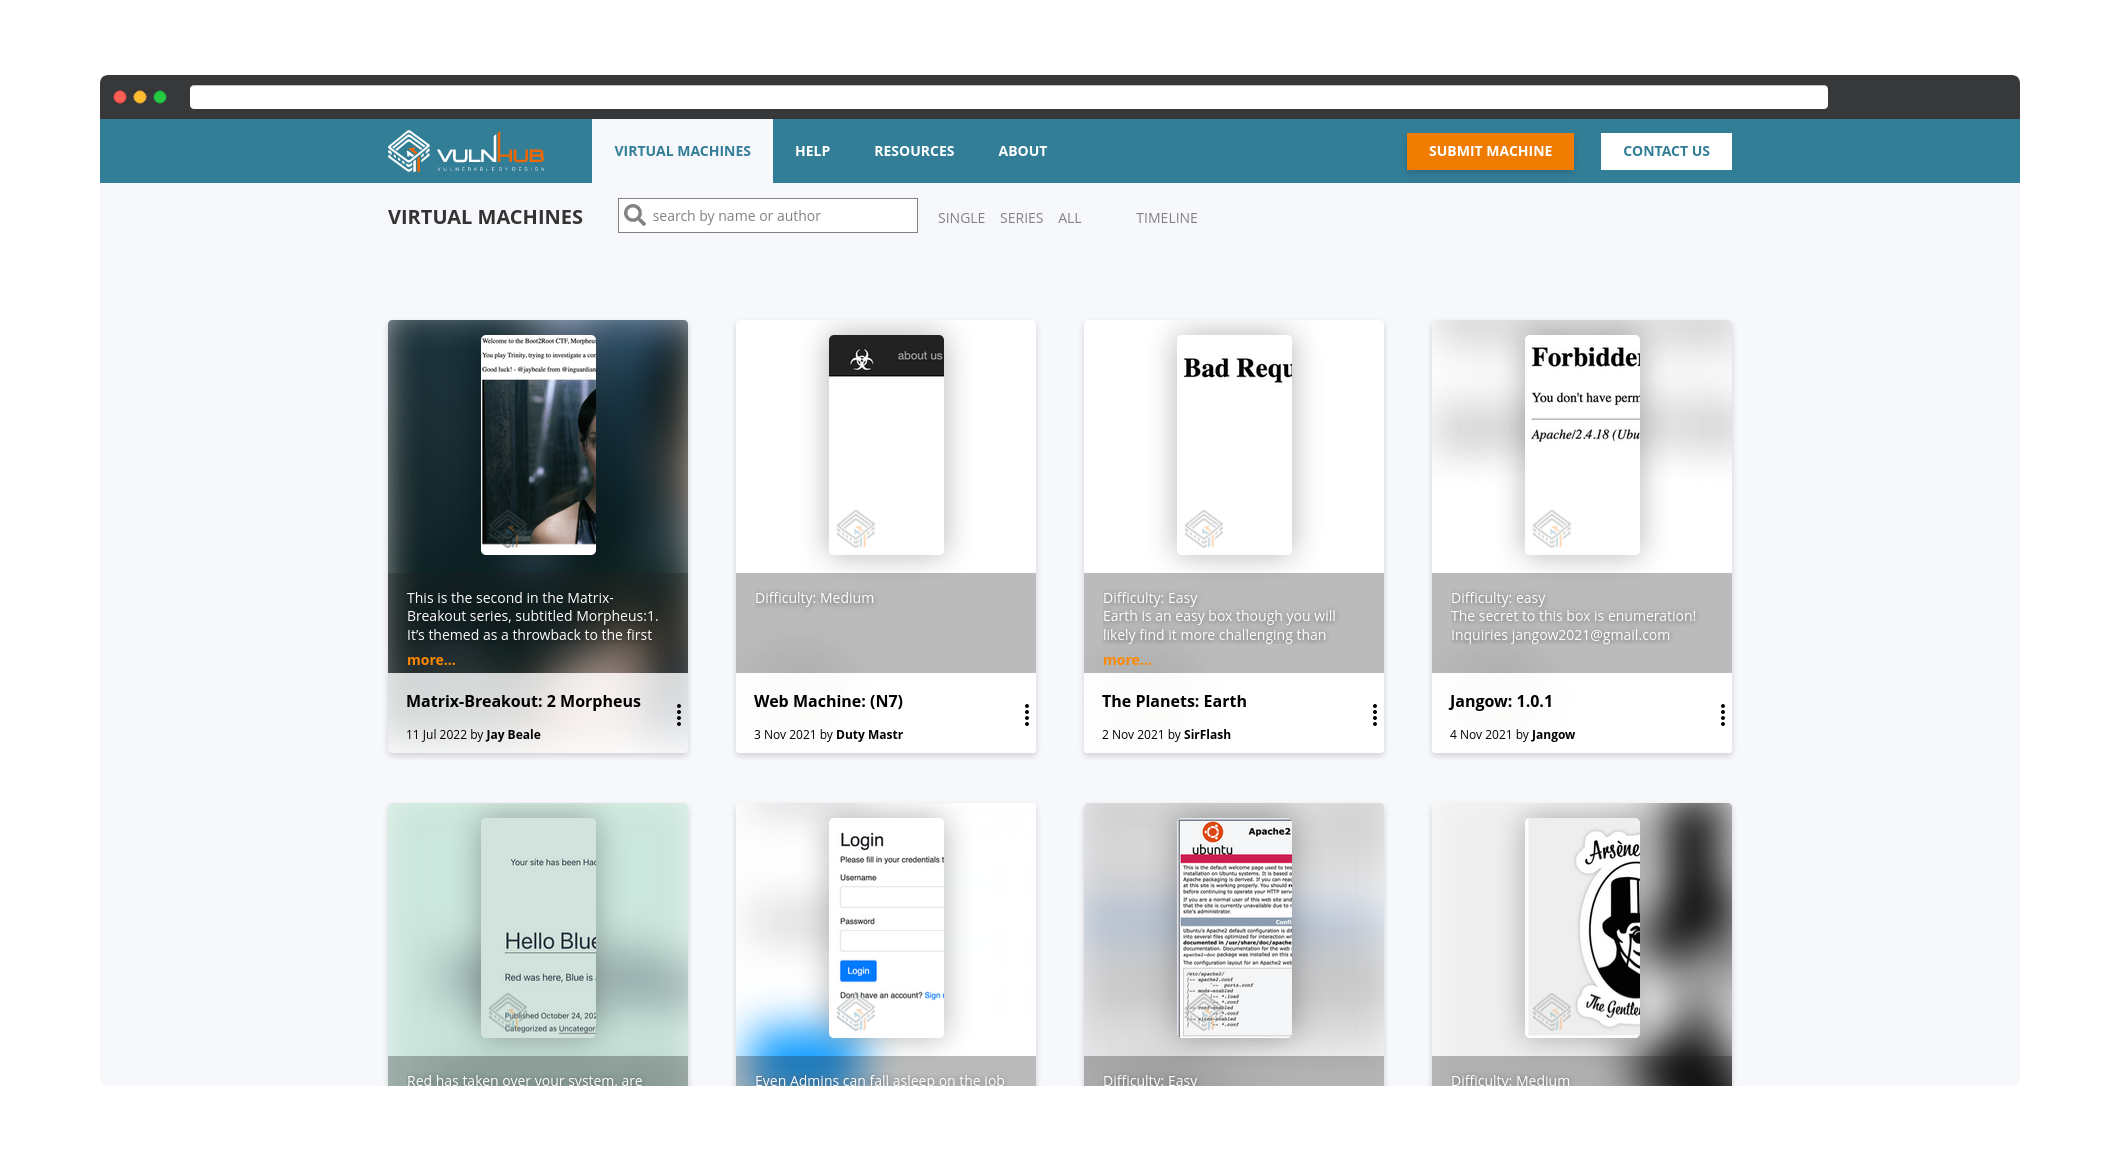
\includegraphics[width=\textwidth]{images/Capturas/Web de VulnHub.png}
            \caption{Web de VulnHub}
            \label{fig:VulnHub-web}
        \end{figure}
        
        Estos desafíos son diseñados por la comunidad, y la plataforma también ofrece la opción de que los usuarios puedan crear y compartir sus propios desafíos y máquinas virtuales.
        
        Al contrario de lo que sucede con otras plataformas, entre ellas Hack The Box y TryHackMe mencionadas anteriormente, \textbf{esta plataforma es completamente gratuita} y todo su contenido está construido por y para los usuarios.
        
        \newpage
    
    
    \section{OverTheWire}
    
        Plataforma de laboratorios \textbf{diseñada de manera progresiva}, donde los usuarios pueden avanzar en su aprendizaje de forma gradual, comenzando con los niveles más fáciles y avanzando hacia los más complejos; cada nivel de desafío presenta un objetivo diferente, haciendo que los usuarios deban usar su ingenio y habilidades en seguridad informática para resolver los desafíos y avanzar al siguiente nivel.
        
        \begin{figure}[h]
            \centering
            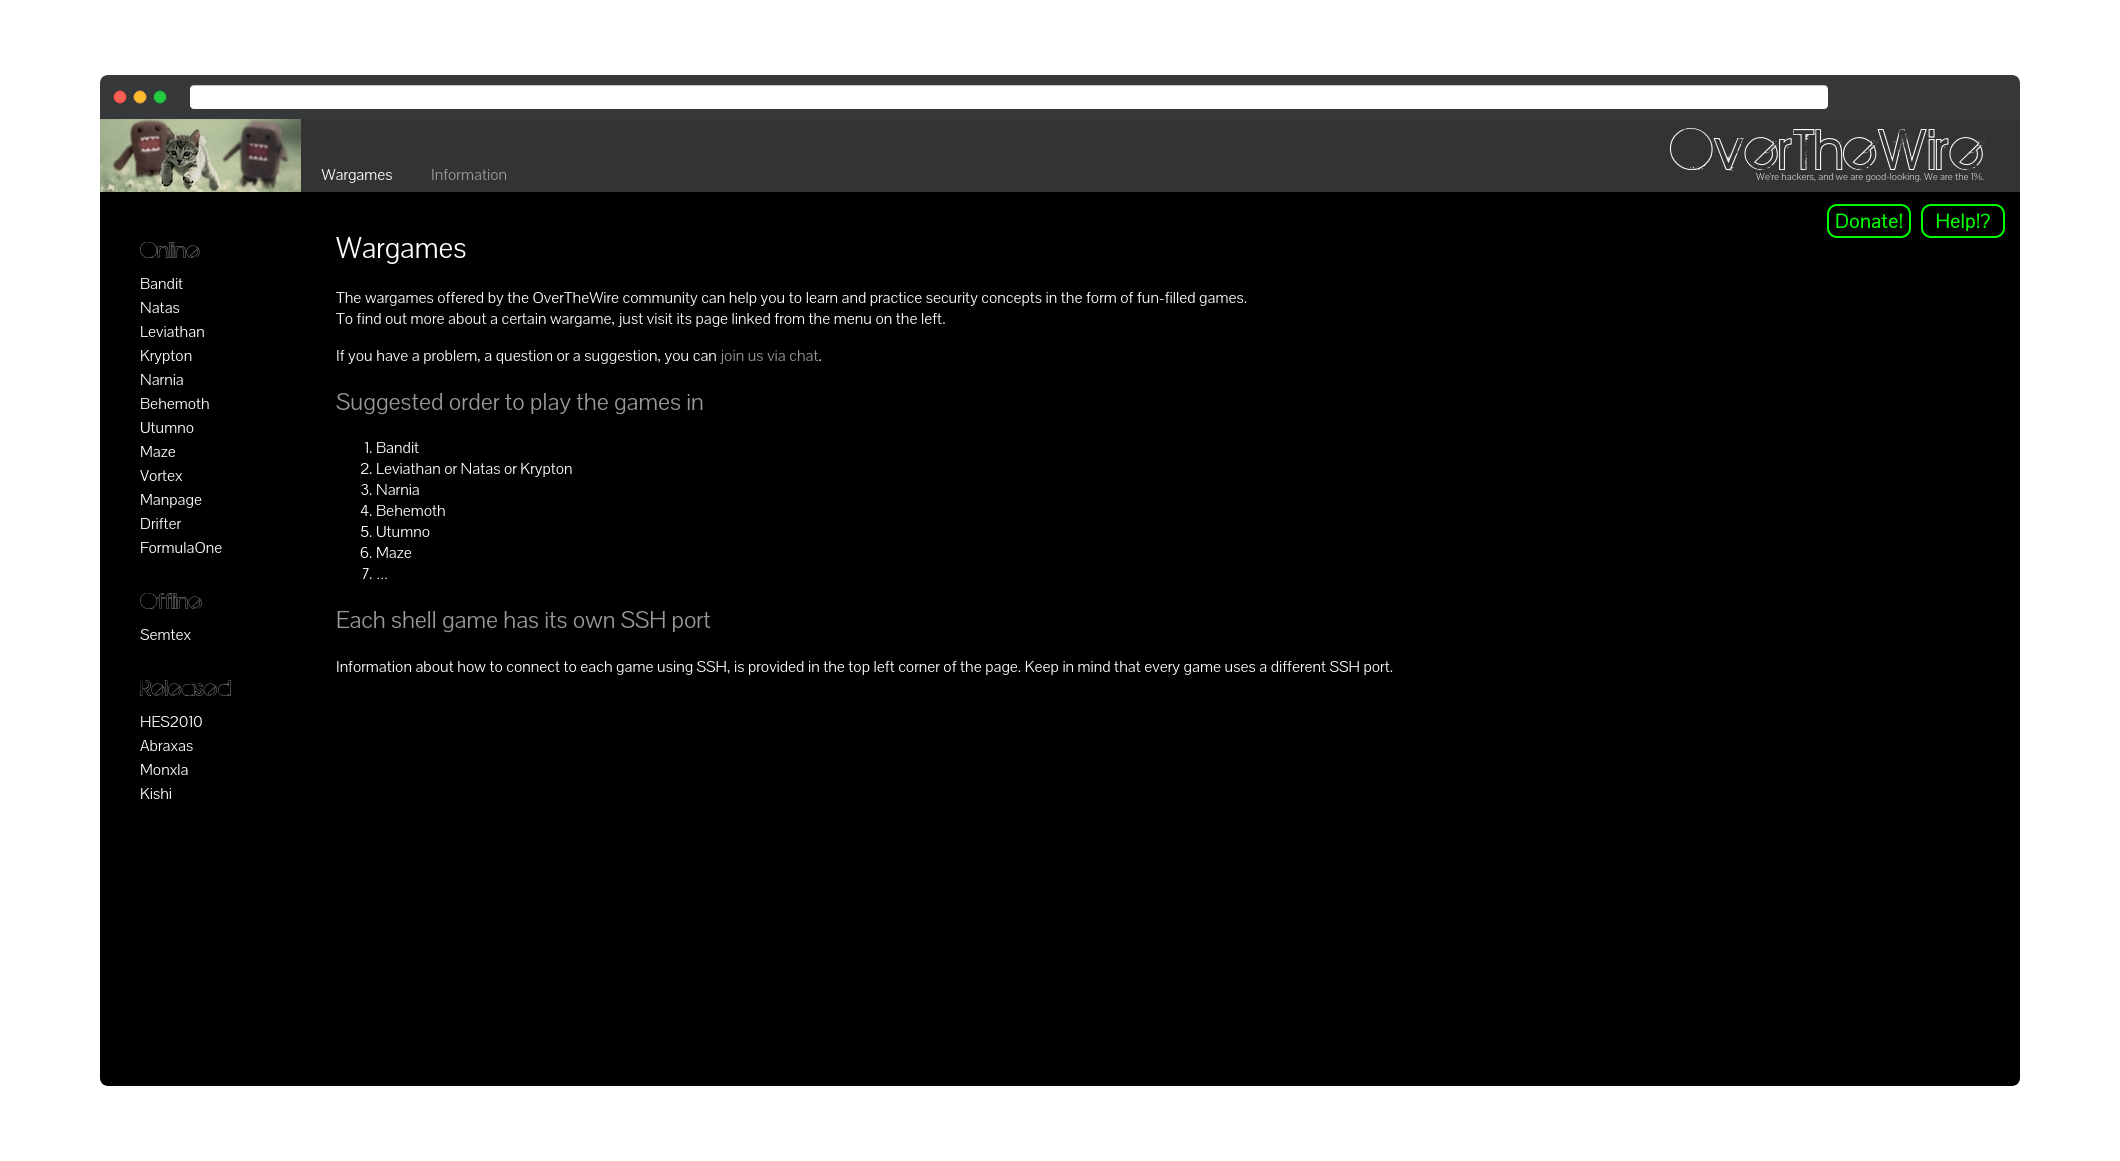
\includegraphics[width=\textwidth]{images/Capturas/Web de OverTheWire.png}
            \caption{Web de OverTheWire}
            \label{fig:OverTheWire-web}
        \end{figure}
        
        Uno de los aspectos únicos de OverTheWire es que los desafíos están diseñados para simular situaciones del mundo real, lo que permite a los usuarios adquirir habilidades prácticas y relevantes para el mundo laboral de la ciberseguridad; pudiendo aplicar lo aprendido a situaciones reales y utilizar sus habilidades para asegurar sistemas y aplicaciones.
        
        Al contrario de lo que sucede con otras plataformas, entre ellas Hack The Box y TryHackMe mencionadas anteriormente, \textbf{esta plataforma es completamente gratuita} y todo su contenido está construido por y para los usuarios.
        
        \cleardoublepage
    
    

\chapter{Investigación previa}
    \label{cap:investigacion-previa}

    \section{Proceso creativo}
        \label{sec:proceso-creativo}

        Antes de comenzar a desarrollar el proyecto, resulta importante saber de forma más específica \textit{qué} se quiere llevar a cabo, y una vez decidio el objetivo, analizar las posibles opciones para conseguirlo.
        
        Ya se realizó una investigación previa sobre las diferentes plataformas de aprendizaje de ciberseguridad existentes -descritas en el Estado del Arte \ref{cap:estado-arte}- con el objetivo de analizar sus características y funcionalidades.
        
        La mayoría -y más conocidas- de estas plataformas son CTFs (Capture The Flag), y aunque son muy útiles para poner en práctica los conocimientos adquiridos, no suelen ofrecer un entorno de aprendizaje guiado, sino que el usuario debe resolver los desafíos por su cuenta, sin ningún tipo de documentación que le ayude a resolverlos, más allá de las pistas que ofrezca la propia plataforma o las soluciones que hayan publicado otros usuarios en Internet.

        Sin embargo, esto no siempre es así, ya que como se vió en el apartado anterior: Try Hack Me \cite{tryhackme} ofrece tanto retos instructivos como retos puramente prácticos y competitivos; mientras que Hack The Box \cite{hackthebox}, la plataforma más reconocida, ha sido capaz de lanzar su propia plataforma educativa con retos guiados: HTB Academy \cite{hackthebox-academy}.

        Teniendo eso cuenta, se plantearon las siguientes ideas para afrontar el proyecto.


        \subsection{Plataforma de CTFs}

            La primera idea planteada fue, precisamente, replicar una plataforma de CTFs (Capture The Flag). Esta versión del proyecto se centraría más en enseñar distintos conceptos de la ciberseguridad al usuario, acompañados de una serie de retos que pondrían a prueba los conocimientos adquiridos; algo parecido a las plataformas TryHackMe y HTB Academy mencionadas en el apartado anterior.

            Esta idea fue descartada porque ya existen muchas plataformas de CTFs, y se pretendía hacer algo distinto con este proyecto. Se requería un entorno de aprendizaje guiado y como se mencionó anteriormente, los CTFs no suelen ofrecerlo.

        
        \subsection{Plataforma como portal de descargas}

            Tomando como ejemplo los retos descargables de la Academia Hacker de Incibe \cite{retos-INCIBE}, se planteó la posibilidad de crear máquinas virtuales y alojarlas en el servidor a modo de elementos descargables; es decir, la plataforma contaría con un sitio web que ofrecería información documentada sobre distintos conceptos de ciberseguridad, pero la virtualización se llevaría a cabo por el propio usuario en su equipo, experimentando localmente.

            Esta idea también fue descartada porque plantea un gran problema de fricción entre el usuario y el objetivo de la plataforma: no existiría la posibilidad de ofrecer un entorno de trabajo en el que el usuario pudiera interactuar con los laboratorios de forma remota y con herramientas aisladas, sino que este debería descargar y configurar un hypervisor, o instalar Docker para acceder a los entornos de prueba en su equipo. Debido a esto, se perdería esa esencia de minimalismo y sencillez que debería ofrecer la plataforma.
            
            Además, plantea otros problemas relacionados con el espacio de almacenamiento (tanto en el servidor como en el equipo del usuario).

            Sin embargo, cabe destacar la existencia herramientas que podrían ser de utilidad para este proyecto, como: Vagrant \cite{vagrant}, que permite automatizar la creación y configuración de máquinas virtuales de forma declarativa; y Vagrant Cloud \cite{vagrant-cloud}, que es un repositorio de máquinas virtuales ya configuradas para instalar usando \texttt{vagrant}. También puede ser útil incluir en la plataforma de una guía introductoria a la configuración de una máquina virtual para tests de intrusión (pentesing) con Kali Linux, ya que si bien no es objeto de este proyecto que los usuarios aprendan sobre virtualización, no se puede ignorar el hecho de que es necesario el uso de máquinas virtuales para el sector de la ciberseguridad.

        
        \subsection{Plataforma de laboratorios}

            Por último, se planteó crear una plataforma de laboratorios con la que el usuario pudiera acceder a distintos entornos de forma remota, sin necesidad de descargar ni configurar nada en su equipo. La plataforma estaría compuesta de un sitio web donde estaría recogida la documentación, mientras que el servidor alojaría los entornos virtualizados asociados a dicha documentación.
            
            La principal diferencia y rasgo a destacar de este planteamiento es que los laboratorios actuarían como \textit{sandboxes}; es decir, aunque un laboratorio estaría planteado para que el usuario pudiera resolver un problema descrito, también ofrecería al usuario contar con un entorno con herramientas preinstaladas en el caso de querer hacer sus propias pruebas sobre un concepto en específico.

            Esta idea fue la que más se acercaba a los objetivos del proyecto, y por tanto fue la que se escogió para su desarrollo: solventaba las fricciones de las ideas anteriores, y además ofrecía un entorno de aprendizaje guiado y práctico, que era el objetivo principal del proyecto.

            \newpage

        \subsection{Sobre Jupyter}

            \subsubsection{Jupyter Notebooks}
                
                Jupyter \cite{jupyter} es un proyecto \textit{open-source} que permite crear documentos interactivos llamados \textit{notebooks} que contienen código ejecutable, ecuaciones, visualizaciones y texto explicativo que sigue un formato de Markdown enriquecido y estructurado en bloques. Estos \textit{notebooks} están basadas en JSON y se pueden compartir con otros usuarios, por lo que se convierten en una herramienta muy útil para la investigación y el análisis de datos, pero sobre todo para la colaboración y el aprendizaje.
            
                Debido a la naturaleza de este proyecto, se planteó la idea de incluir páginas en la plataforma que fueran Jupyter Notebooks, de esta forma el usuario podría acceder a la página que contendría documentación y código anidado (característica principal de Jupyter), y en ella podría insertar y ejecutar código, así como generar distintos recursos de forma interactiva para que el usuario pudiera experimentar con ella.

                Sin embargo, se descartó la idea ya que no constituía una prioridad en el desarrollo del proyecto y sus casos de uso eran muy limitados, puesto que el código verdaderamente importante sería ejecutado en las \textit{sandboxes}.
                

            \subsubsection{JupyterHub}

                JupyterHub \cite{jupyterhub} es una aplicación que permite crear un entorno de Jupyter Notebooks en un servidor remoto, de forma que los usuarios puedan acceder a él a través de un navegador web. Esta aplicación es muy útil para la colaboración y el aprendizaje, ya que permite a los usuarios compartir documentos y ejecutar código en un entorno seguro y controlado.
                
                Siguiendo con lo mencionado en el apartado anterior, se planteó la idea de usar JupyterHub para crear distintos entornos de Jupyter Notebook en la nube para que los usuarios pudieran acceder a un entorno de Jupyter Notebooks en el que pudieran ejecutar código y experimentar con los recursos generados por el sistema, en lugar de integrarlos en la plataforma.

                Esta idea también se descartó por ser ser una versión más compleja de la anterior.
                
                \newpage

                
        \subsection{Sobre Docker}

            Docker, descrito en la sección \ref{sec:docker}, permitiría la creación de contenedores para los distintos laboratorios.
                
            Esta idea surgió a partir del artículo \textit{Cyber Security Testbeds and Malware Testing} \cite{securitylab-malware-analysis} de la Universidad de Trento, donde un grupo de investigación realizaban un estudio sobre los efectos de un \textit{exploit} de una aplicación sobre varias versiones de la misma y usada en distintos entornos de desarrollo.

            \begin{quotation}
                
                Given a software environment $E$, an exploit $X$ that successfully subverts an application $A$, that is running on $E$:
                
                \begin{itemize}
                    \item Will $X$ be successful on an application $A$ running on another environment $E'$?
                    \item Will $X$ be successful on another version of $A$, $A'$, running on $E$?
                    \item Will $X$ be successful on another version of $A$, $A'$, running on $E'$?
                \end{itemize}

            \end{quotation}

            Para ello, el grupo de investigación desarrolló un conjunto de pruebas a partir de contenedores, usando combinaciones de un \textbf{conenedor principal} junto a \textbf{contenedores secundarios}.

            \begin{quote}

                Instead of creating separate virtual machines for every application/configuration we use the Linux Containers technology that provides virtualization capabilities on the operation system level. \[...\] We use Docker to implement two types of containers: (1) software-specific that contain operating system, webserver and database engine; (2) application-specific that is build on top of a desired software-specific container and also encapsulates the application files. The figure on the right shows an example Wordpress3.2 application container that has been built on top of the “ubuntu-apache-mysql” software container.

            \end{quote}

            Y la figura que representa dicho planteamiento es la siguiente:

            \begin{figure}[htbp]
                \centering
                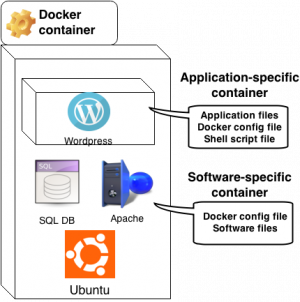
\includegraphics[scale=0.75]{images/Diagramas/Articulo.png}
                \caption{Contenedor de Wordpress3.2 sobre contenedor con Ubuntu + Apache + MySQL}
                \label{fig:articulo}
            \end{figure}

            \newpage
            

            \subsubsection{Red de contenedores de Docker}

                Inicialmente se interpretó el sistema del artículo anterior como una red de contenedores.
                
                Por tanto, en lugar de crear un contenedor para cada \textit{sandbox}, se planteó la idea de crear una red contenedores para cada laboratorio, de forma que cada red estuviera compuesta por aquellos elementos a tratar en dicho laboratorio, y que a su vez sería accesible desde el exterior a través de un puerto específico, permitiendo a un usuario conectarse a través de SSH.

                Esto podría lograrse usando Docker Compose \cite{docker-compose}, que permite crear y ejecutar aplicaciones Docker de forma sencilla, usando un archivo YAML que describe los servicios que componen la aplicación, así como las dependencias entre ellos.

                Visto en perspectiva, queda bastante claro que el mecanismo del proyecto planteado en el artículo y el propuesto en esta sección no son similares más allá del uso de contenedores.
                
                
            \subsubsection{Dependencia de contenedores de Docker}

                Por tanto, el planteamiento inicial de usar una red de contenedores era errónea.
                
                La estructura descrita en el artículo se forma a través del uso de la tecnología de contenedores de Linux, alojando cada aplicación y configuración de software en un contenedor.

                Una posible réplica de ese mecanismo podría realizarse de la siguiente forma:

                \begin{enumerate}

                    \item \textbf{Instalar Docker en el sistema operativo}
                    
                    Realizable siguiendo las instrucciones de instalación en el sitio web oficial de Docker.
                
                    \item \textbf{Crear imágenes específicas del software}
                    
                    Realizable utilizando un archivo Dockerfile que describa la configuración y los componentes que deben incluirse en dicha imagen.

                    \item \textbf{Crear un contenedor específico de la aplicación}

                    Para crear este tipo de contenedor, se debe construir sobre un contenedor específico del software previamente creado; para ello, se deben encapsular los archivos de la aplicación dentro del contenedor específico del software.

                    \item \textbf{Ejecutar contenedores}
                    
                    Una vez creados los contenedores específicos del software y de la aplicación, pueden ejecutarse con el comando \texttt{docker run} de Docker.

                \end{enumerate}

                En el paso 2 se crea una imagen específica del software a partir de un archivo Dockerfile que describe la configuración y los componentes que deben incluirse en los contenedores resultantes de dicha imagen.

                En el paso 3, se crea una imagen específica de la aplicación que se construye sobre la imagen del software previamente creada; es decir, se crea una nueva imagen que constituye una capa de configuración adicional sobre la configuración de la propia imagen del software, que actua como base. Esta nueva imagen encapsula los archivos de la aplicación y se crea también a partir de un archivo Dockerfile.

                El resultado final es un contenedor específico de la aplicación que reutiliza el sistema operativo y los componentes incluidos en la imagen del software, pero que añade los archivos específicos para el funcionamiento de la aplicación.

                A continuación se muestran 2 pseudo-códigos que representan el resultado final descrito:

                \begin{figure}[!htbp]
                    \centering
                    
                    \begin{subfigure}[!htbp]{\textwidth}
                        \centering
                        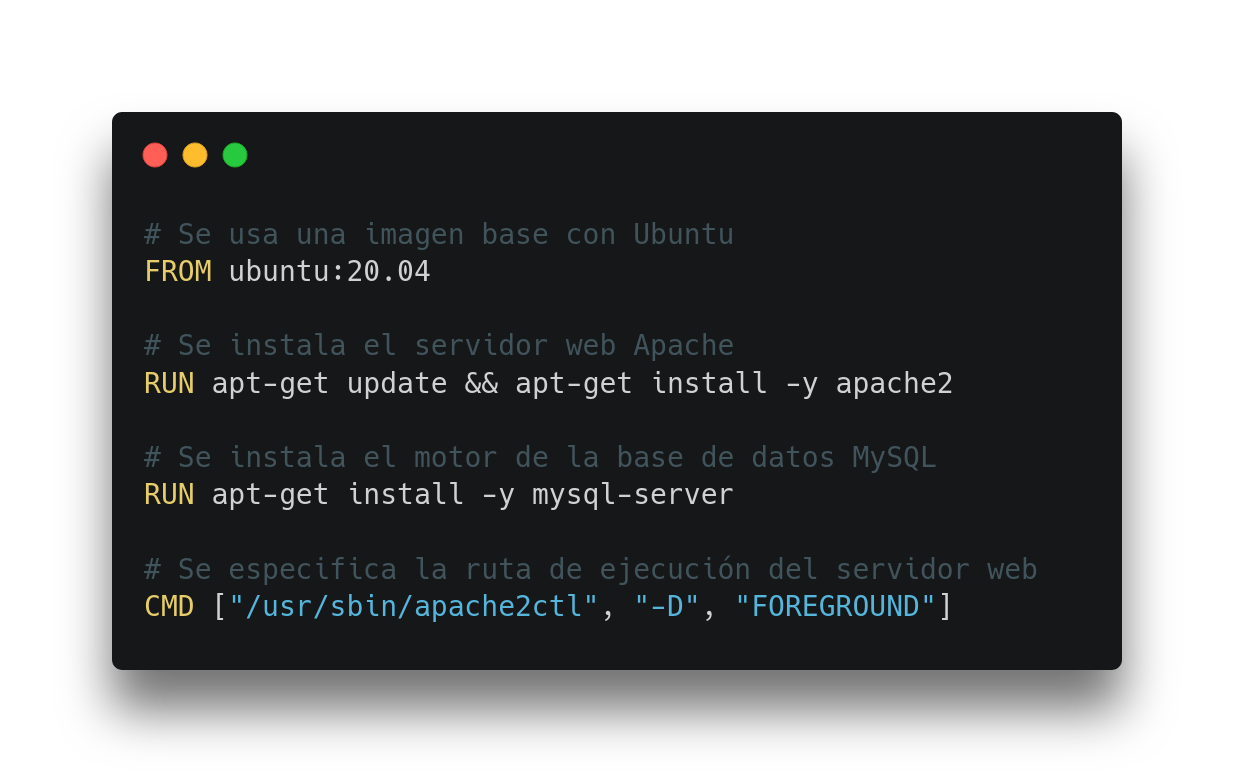
\includegraphics[width=0.8\textwidth]{images/Contenedor A.png}
                        \caption{Dockerfile de una imagen principal (padre)}
                    \end{subfigure}
                    
                    \begin{subfigure}[!htbp]{\textwidth}
                        \centering
                        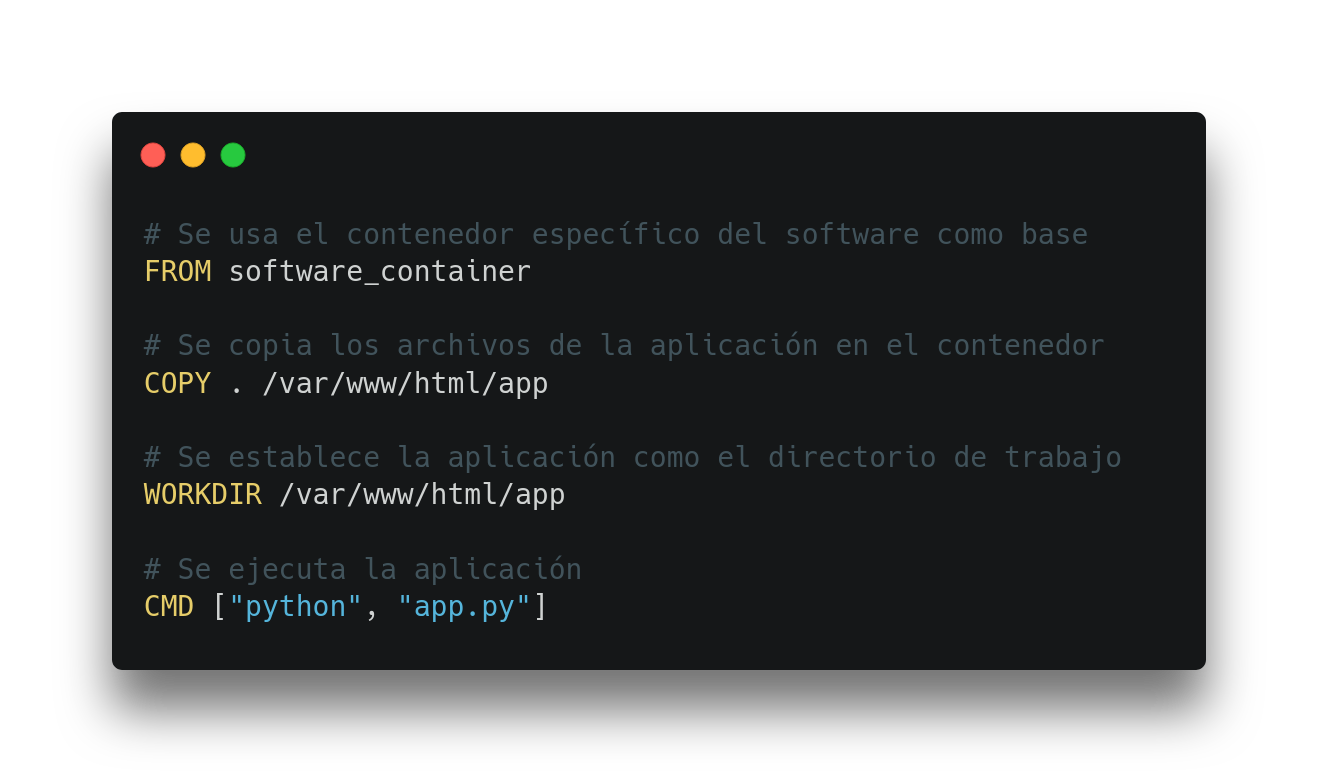
\includegraphics[width=0.8\textwidth]{images/Contenedor B.png}
                        \caption{Dockerfile de una imagen secundaria (hija)}
                    \end{subfigure}
                    
                    \caption{Dependencia de contenedores}
                    \label{fig:dependencia-contenedores}
                \end{figure}
                
                El Dockerfile de la imagen hija hace referencia a la imagen padre mediante la línea $\texttt{FROM software\_container}$, estableciendo la dependencia. Además, se copian los archivos de la aplicación en la imagen y se establece como el directorio de trabajo. Finalmente, se ejecuta la aplicación con la línea $\verb|CMD ["python", "app.py"]|$, lo que mantendrá activos los contenedores resultantes de dicha imagen.

                \begin{figure}[!htbp]
                    \centering
                    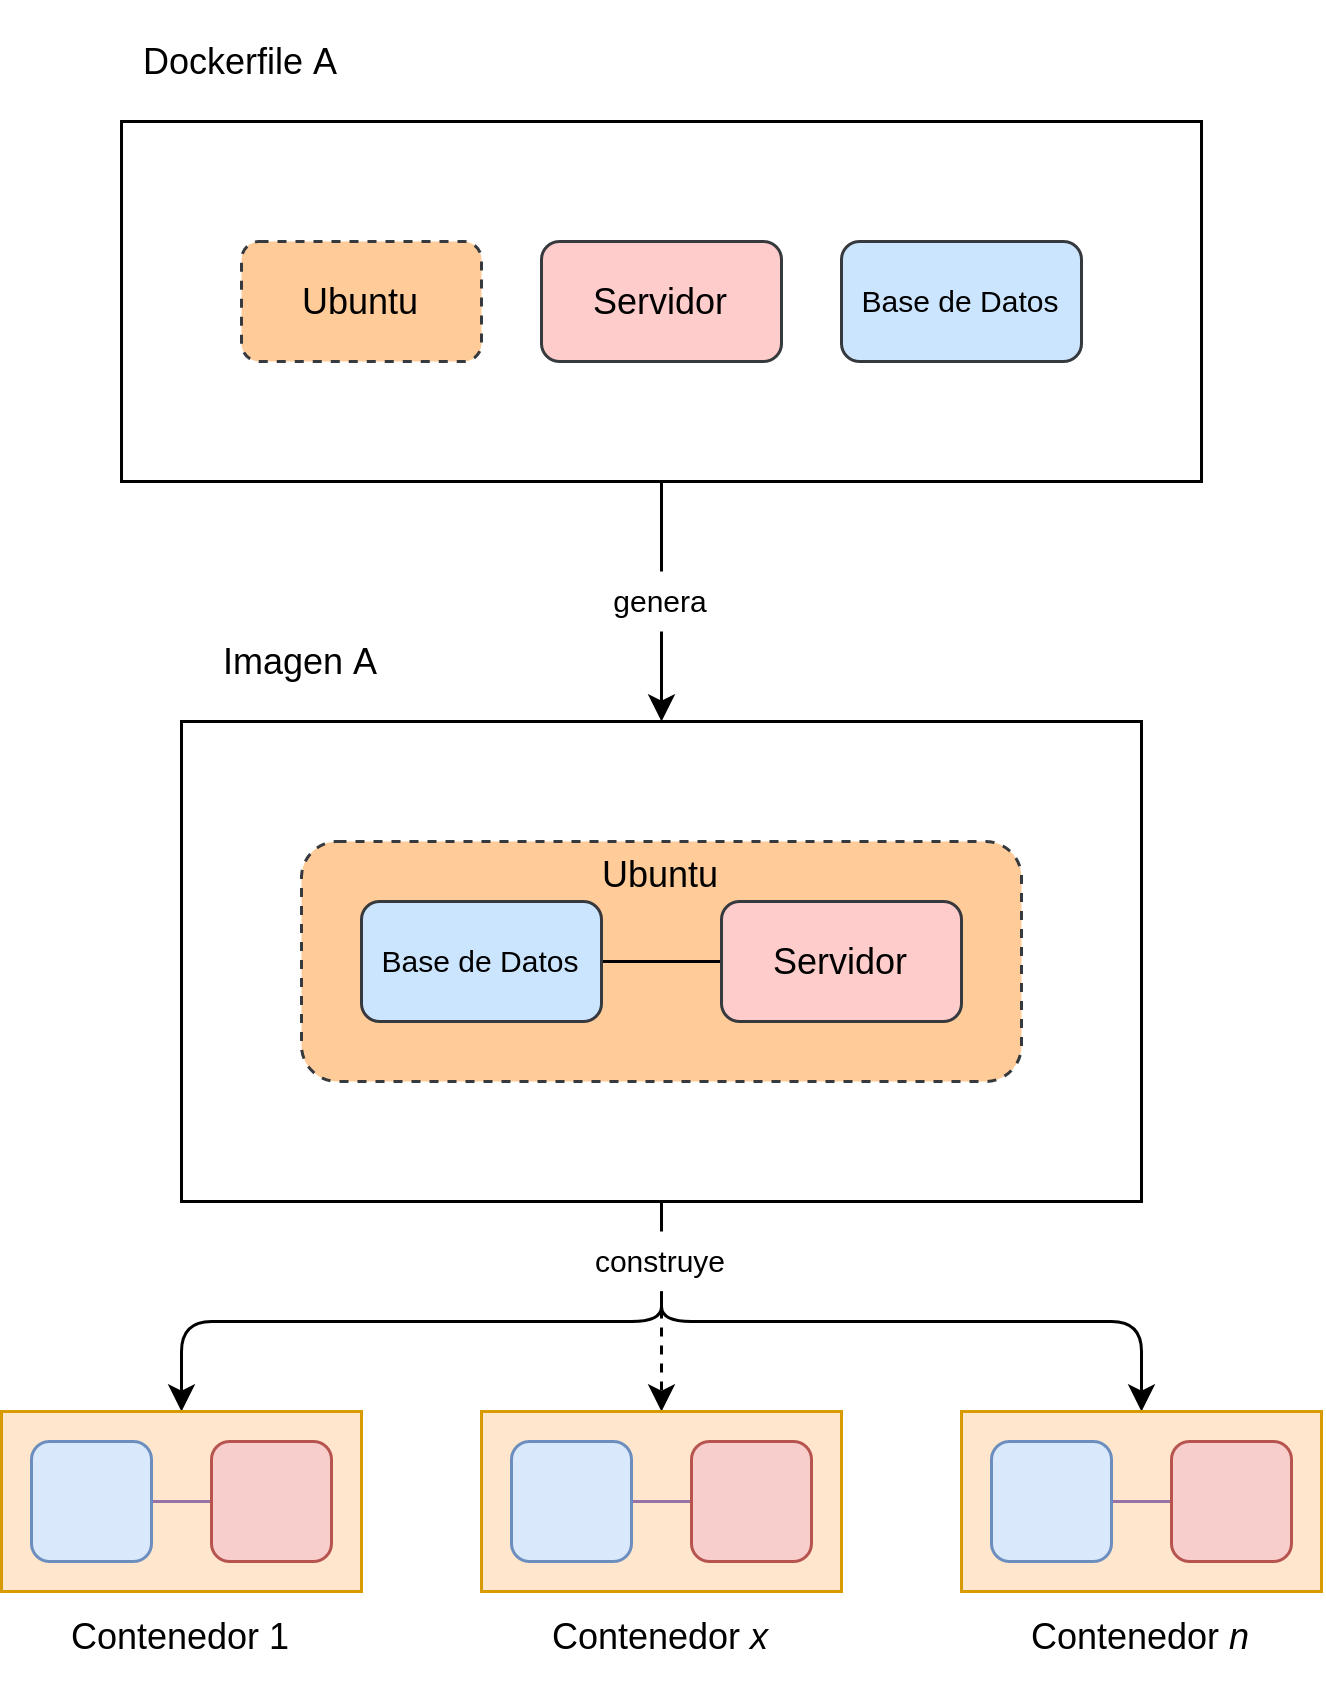
\includegraphics[scale=0.14]{images/Diagramas/Contenedor A.png}
                    \caption{Creación de contenedores principales (padres)}
                    \label{fig:contenedor-padre}
                \end{figure}
                
                \begin{figure}[!htbp]
                    \centering
                    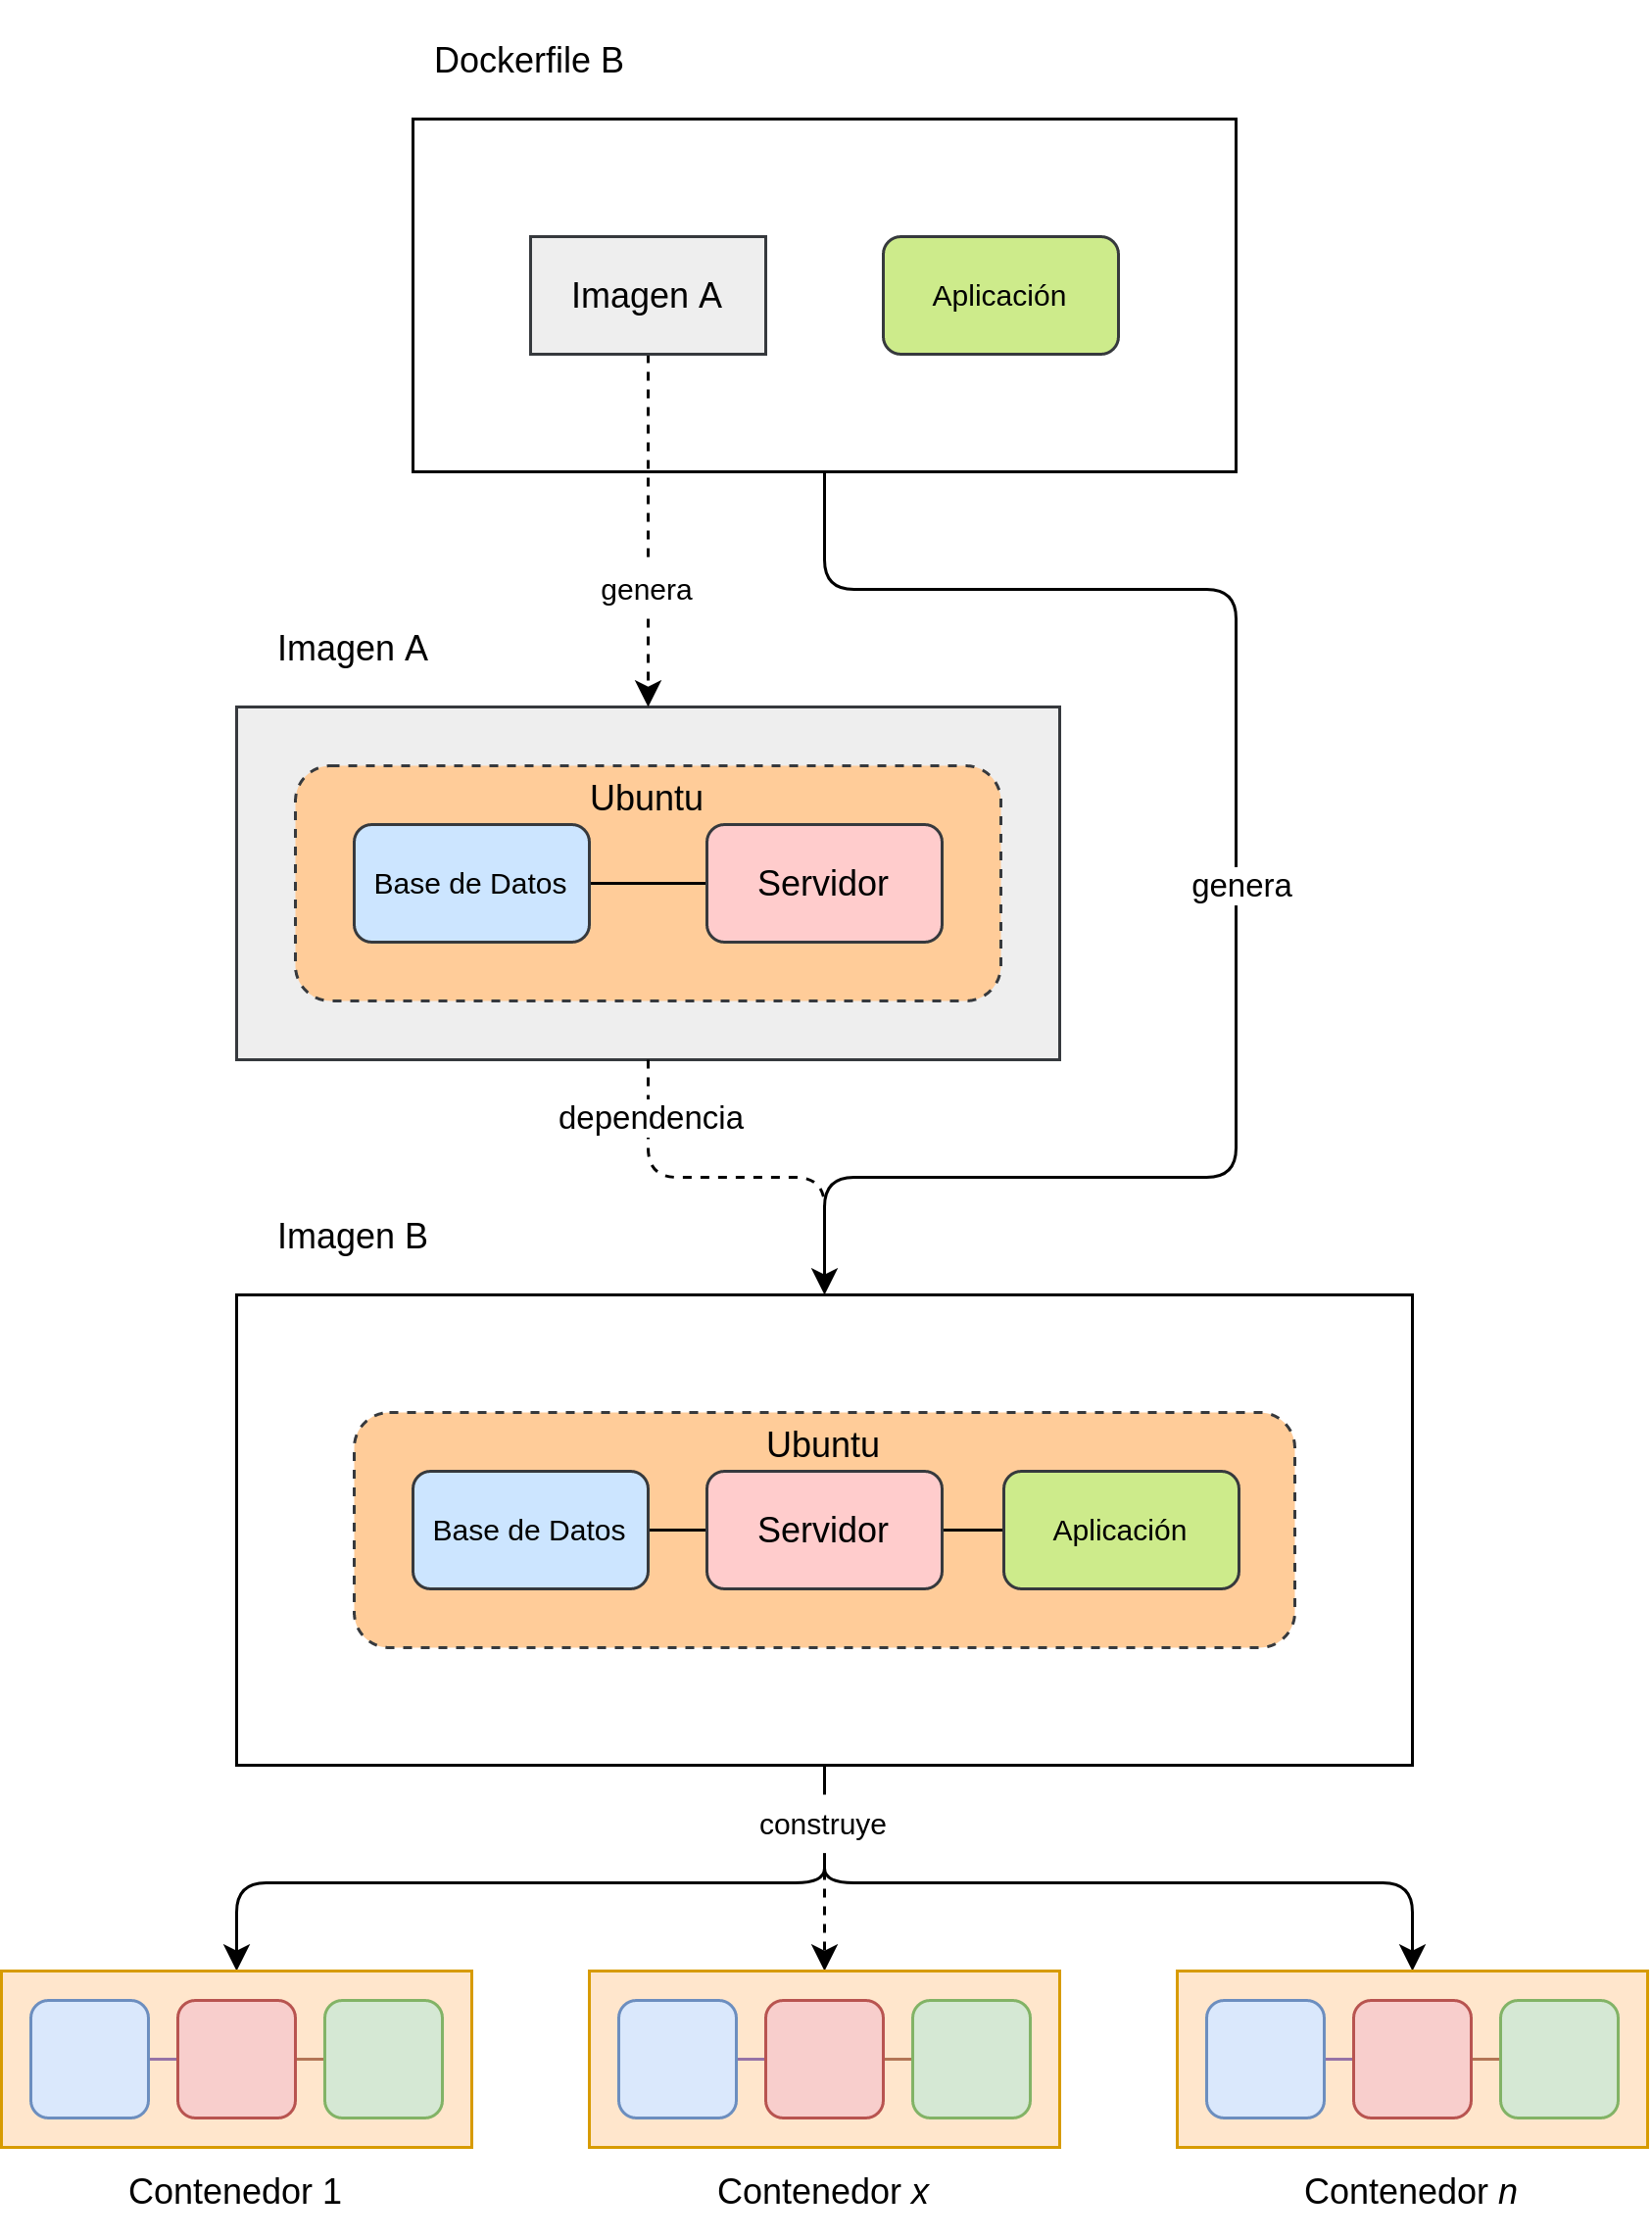
\includegraphics[scale=0.14]{images/Diagramas/Contenedor B.png}
                    \caption{Creación de contenedores secundarios (hijos)}
                    \label{fig:contenedor-hijo}
                \end{figure}
                
                \newpage


    
    \section{Análisis de Tecnologías}
        
        \subsection{Página web}

            \begin{table}[!htbp]
                \centering
                
                \small
                
                \begin{tabular}{|>{\centering\arraybackslash}m{3cm}|>{\centering\arraybackslash}m{3.5cm}|>{\centering\arraybackslash}m{3.5cm}|>{\centering\arraybackslash}m{3.5cm}|}
                    \hline
                    \textbf{Características} & \textbf{WordPress} & \textbf{Astro} & \textbf{Drupal} \\
                    \hline
                    \hline
                    \textbf{Tipo de plataforma} & CMS & Framework & CMS \\
                    \hline
                    \textbf{Orientación} & Sitios web: pequeños y medianos & Aplicaciones web & Sitios web: grandes y complejos\\
                    \hline
                    \textbf{Lenguaje de programación} & PHP & Javascript & PHP \\
                    \hline
                    \textbf{Facilidad de uso} & Simple: no requiere experiencia técnica ni programación & Compleja: requiere experiencia técnica y en programación & Compleja: requiere experiencia con el propio CMS \\
                    \hline
                    \textbf{Personalización} & Alta: temas y plugins & Muy alta: desarrollo web & Alta: módulos y extensiones \\
                    \hline
                    \textbf{Escalabilidad} & Sí: sitios web pequeños y medianos & Sí: aplicaciones web pequeñas y grandes & Sí: sitios grandes y complejos \\
                    \hline
                    \textbf{Comunidad} & Grande: usuarios y desarrolladores & Creciente: desarrolladores & Mediana: usuarios y desarrolladores, muy dedicados y comprometidos \\
                    \hline
                    \textbf{Popularidad} & El CMS más popular & Un framework relativamente nuevo & Uno de los CMS más usados \\
                    \hline
                    \textbf{Seguridad} & Alta: pero es vulnerable a ataques por su popularidad & Variable: depende de la implementación del desarrollador & Alta: CMS centrado en la seguridad y la protección \\
                    \hline
                \end{tabular}
                
                \caption{Comparativa entre WordPress, Astro y Drupal}
                \label{tab:wordpress-vs-astro-vs-drupal}
            \end{table}

            Se ha elegido WordPress como la plataforma para la creación de la página web del proyecto debido a sus ventajas en cuanto a facilidad de uso, personalización y escalabilidad, que eran los principales aspectos a tener en cuenta para el desarrollo.

            
            \subsubsection{WordPress y Astro}

                \paragraph{Facilidad de uso}
                    
                    Factor importante en la decisión de elegir esta herramienta ya que no se cuentan con conocimientos previos de programación web ni a nivel técnico, por lo que debía usarse una herramienta que no tuviera en cuenta esas necesidades.
                    
                    WordPress parece cubrir ese aspecto de forma notable debido a que su popularidad se basa, precisamente, en la cantidad de usuarios que son capaces de crear una página web sin necesidad de ser desarrolladores o contar con experiencia previa.
                
                \paragraph{Personalización}
                
                    También fue considerada un factor clave ya que se contaba con la creación de una página web atractiva y funcional.
                    
                    Teniendo en cuenta lo mencionado en el punto anterior acerca de la falta de conocimientos previos, se hubiera empleado una gran cantidad de tiempo no solo en aprender a elaborar un buen \textit{frontend} desde cero, sino que el objetivo principal de este trabajo de fin de grado no se centra tanto en la página web, sino en el sistema completo, pudiendo considerar la mejora del \textit{frontend} como una posible futura línea de trabajo \ref{sec:futuras-lineas-trabajo}.
                
                \paragraph{Escalabilidad}
                
                    Si bien este proyecto constituye una prueba de concepto, uno de los objetivos \ref{sec:objetivos} a tener en cuenta se trataba de construir una plataforma web fácilmente extensible.

                    La escalabilidad de WordPress es una de sus principales fortalezas y uno de los motivos por los que es una plataforma popular y confiable para la creación de sitios web de cualquier tamaño. Su arquitectura modular y su capacidad para trabajar con bases de datos y servidores de alta gama, la convierten en opción sólida para aquellos que buscan crear sitios web que puedan crecer y adaptarse a sus necesidades en el futuro.


            \subsubsection{WordPress y Drupal}

                También se tuvo en cuenta Drupal \cite{drupal}, otro CMS \textit{open-source} que se encuentra entre los más populares y que, a pesar de no ser tan conocido como WordPress, también es una opción muy interesante para la creación de páginas web.

                \paragraph{Facilidad de uso, personalización y escalabilidad}
                
                    Observando la tabla anterior se puede apreciar varios motivos por los que se ha optado usar Wordpress en lugar de Drupal, pero todos ellos relacionados al mismo punto: \textbf{la complejidad de Drupal no se ajusta a las necesidades de este proyecto}.
    
                    Si bien puede ser una idea interesante a largo plazo y en un hipotético caso de evolución de la plataforma web a un proyecto superior, para una prueba de concepto como la que se está llevando a cabo, se debe optar por una herramienta más sencilla y fácil de usar.
    
                    \newpage
    

        \subsection{Base de Datos}
        
            \subsubsection{SQLite vs MySQL}

                SQLite es un RDBMS \cite{sqlite} que se caracteriza por ser ligero, rápido y fácil de usar; se trata de una buena opción para proyectos pequeños, pero no es recomendable para proyectos de gran envergadura, ya que no es capaz de manejar grandes cantidades de datos.
                
                Por otro lado, MySQL también es otro RDBMS \cite{mysql} que se caracteriza por ser rápido, seguro y fácil de usar; al contrario que con SQLite, MySQL sí es recomendable para proyectos de gran envergadura, ya que es capaz de manejar grandes cantidades de datos.

                \begin{table}[h]
                    \centering
                    
                    \begin{tabular}{|>{\centering\arraybackslash}m{4cm}|>{\centering\arraybackslash}m{5cm}|>{\centering\arraybackslash}m{5cm}|}
                        \hline
                        \textbf{Características} & \textbf{SQLite} & \textbf{MySQL} \\
                        \hline
                        \hline
                        \textbf{Tipo de base de datos} & Relacional, integrada & Relacional, cliente-servidor \\
                        \hline
                        \textbf{Gestión de usuarios} & Debe programarse & Integrada \\
                        \hline
                        \textbf{Escalabilidad} & Limitada: por su naturaleza integrada & Escalable: en función del hardware disponible \\
                        \hline
                        \textbf{Confiabilidad} & Menor capacidad de recuperación de datos & Mayor capacidad de recuperación de datos \\
                        \hline
                        \textbf{Flexibilidad} & Limitada en cuanto a configuración de memoria & Mayor flexibilidad en configuración \\
                        \hline
                        \textbf{Seguridad} & Limitada: no ofrece encriptación de datos & Mayor seguridad: ofrece encriptación de datos \\
                        \hline
                    \end{tabular}
                        
                    \caption{Comparativa entre SQLite y MySQL.}
                    \label{tabla:mysql-vs-sqlite}
                \end{table}

                En función de la naturaleza del proyecto a realizar, se ha considerado usar MySQl debido a las siguientes razones:
                    
                \paragraph{Gestión de usuarios integrada}
                    
                    Al tratarse de una plataforma web que requiere la gestión de usuarios, MySQL ofrece una gestión de usuarios integrada, lo que simplifica y agiliza el proceso de gestión de usuarios en comparación con SQLite.
                
                \paragraph{Escalabilidad}
                    
                    MySQL ofrece una mayor escalabilidad que SQLite debido a su arquitectura cliente-servidor. Esto significa que puede manejar grandes cantidades de datos y muchos usuarios de manera simultánea, lo que es importante en un entorno en el que se espera que varios usuarios se conecten y utilicen la plataforma al mismo tiempo.

                \paragraph{Confiabilidad}
                    
                    MySQL ofrece una mayor capacidad de recuperación de datos en comparación con SQLite. Esto es importante en un proyecto que busca ser utilizado por varias personas, ya que cualquier pérdida de datos podría tener un impacto significativo.

                \paragraph{Seguridad}
                    
                    MySQL ofrece mayor seguridad que SQLite al contar con encriptación de datos. Esto es importante en un proyecto que busca proteger los datos de los usuarios y prevenir posibles ciberataques.

                Además, también se ha tenido en cuenta su integración con WordPress, herramienta sleccionada para la página web de la plataforma, ya que WordPress cuenta con integración inmediata con MySQL desde su instalación.    


        \subsection{Alojamiento}

            \subsubsection{Local}

                Inicialmente, se planteó el uso de un servidor local para el alojamiento de la plataforma web, lo que permite realizar pruebas de forma maś rápida y sencilla, sin necesidad de contratar un servidor externo.

                Actualmente, esta es la opción que se está utilizando para el proyecto, pero se espera trasladarlo a una plataforma cloud para que este sea accesible públicamente, primeramente para beta-testers y posteriormente, usuarios finales.

                
            \subsubsection{Linode}

                Esta empresa ofrece servicios de alojamiento en la nube mediante servidores virtuales privados (VPS) con diferentes características y precios, lo que permite a los usuarios elegir el plan que mejor se adapte a sus necesidades.

                Se presenta a sí misma como la alternativa a \textit{AWS} \ref{sec:aws}.

                Además, Linode cuenta con una interfaz de usuario intuitiva y fácil de usar, así como con una amplia documentación y soporte técnico para ayudar a los usuarios a configurar y administrar sus servidores.

                \begin{figure}[htbp]
                    \centering

                    
\includegraphics[width=0.15\textwidth]{images/Logos/linode.png}
                    \caption{Logo de Linode.}

                    \label{fig:linode-logo}
                \end{figure}

                Este proyecto requiere la gestión de contenedores Docker, por lo que se buscaba un servicio que integrara Kubernetes para facilitar la gestión de los mismos.
                
                Linode ofrece un servicio de Kubernetes que permite a los usuarios implementar y administrar clústeres de Kubernetes en la nube.

                \paragraph{Linode Kubernetes Engine (LKE)}

                    Este servicio se encarga de la configuración, el aprovisionamiento y la administración de los nodos del clúster, lo que permite a los usuarios centrarse en el desarrollo de sus aplicaciones en lugar de en la gestión de la infraestructura subyacente.
                    
                    \begin{figure}[htbp]
                        \centering
    
                        
\includegraphics[width=0.15\textwidth]{images/Logos/lke.png}
                        \caption{Logo de Linode Kubernetes Engine.}
    
                        \label{fig:lke-logo}
                    \end{figure}
                    
                    Además, Linode Kubernetes Engine (LKE) es compatible con herramientas y servicios de terceros, lo que permite a los usuarios integrar fácilmente sus aplicaciones con otros servicios en la nube.


            \subsubsection{Amazon Web Service (AWS)}
                \label{sec:aws}

                Esta plataforma de servicios en la nube ofrece una amplia gama de servicios, incluyendo almacenamiento, bases de datos, redes, análisis, aprendizaje automático, etc.
                
                AWS permite a los usuarios crear aplicaciones escalables y de alta disponibilidad sin necesidad de invertir en hardware o infraestructura física.

                \begin{figure}[htbp]
                    \centering

                    
\includegraphics[width=0.15\textwidth]{images/Logos/aws.png}
                    \caption{Logo de AWS.}

                    \label{fig:aws-logo}
                \end{figure}

                Como se mencionó anteriormente, este proyecto requiere la gestión de contenedores Docker, por lo que se buscaba un servicio que integrara Kubernetes para facilitar la gestión de los mismos.

                AWS cuenta con el servicio Amazon Elastic Kubernetes Service (EKS), que permite a los usuarios implementar y administrar clústeres de Kubernetes en la nube.

                \paragraph{Amazon Elastic Kubernetes Service (EKS)}

                    Este servicio se encarga de la configuración, el aprovisionamiento y la administración de los nodos del clúster, lo que permite a los usuarios centrarse en el desarrollo de sus aplicaciones en lugar de en la gestión de la infraestructura subyacente. 
                    
                    \begin{figure}[htbp]
                        \centering
    
                        
\includegraphics[width=0.15\textwidth]{images/Logos/eks.png}
                        \caption{Logo de Amazon Elastic Kubernes Services.}
    
                        \label{fig:eks-logo}
                    \end{figure}


            \subsubsection{Google Cloud Platform (GCP)}

                Esta plataforma de Google ofrece una gran cantidad de servicios en la nube con la que poder alojar distintos proyectos en función de sus necesidades: almacenamiento, bases de datos, redes, análisis, aprendizaje automático, etc.
                
                Permite a los usuarios crear aplicaciones escalables y de alta disponibilidad sin necesidad de invertir en hardware o infraestructura física.

                \begin{figure}[htbp]
                    \centering

                    
\includegraphics[width=0.15\textwidth]{images/Logos/gcp.png}
                    \caption{Logo de Google Cloud Platform.}

                    \label{fig:gcp-logo}
                \end{figure}

                Se planteó el uso de esta herramienta para el alojamiento del proyecto porque ofrece un saldo gratuito equivalentes a 3 meses de uso sus servicios, resultando muy interesante para el desarrollo del mismo.

                Cuenta con varios servicios potencialmente compatibles con el proyecto, de los cuales se analizaron los siguientes:

                \paragraph{Google Kubernetes Engine (GKE)}

                    Este servicio permite ejecutar aplicaciones en contenedores de forma sencilla y rápida, sin necesidad de gestionar la infraestructura subyacente.

                    \begin{figure}[htbp]
                        \centering

                        
\includegraphics[width=0.15\textwidth]{images/Logos/gke.png}
                        \caption{Logo de Google Kubernetes Engine.}
                        
                        \label{fig:gke-logo}
                    \end{figure}

                    Este servicio se planteó como una opción para la gestión de los contenedores Docker que son los laboratorios del proyecto.

                    Sin embargo, se descartó esta opción debido a que la complejidad de la herramienta no se ajustaba a las necesidades del proyecto, ya que se buscaba una herramienta que facilitara la gestión de los contenedores Docker, pero de forma más sencilla.

                \paragraph{Google Cloud Run}

                    Este servicio de computación sin servidor (\textit{serverless}) de Google a los desarrolladores implementar fácilmente aplicaciones en contenedores en un entorno completamente administrado, sin la necesidad de administrar la infraestructura subyacente.
                    
                    Cloud Run es compatible con contenedores basados en Docker, lo que significa que es posible empaquetar una aplicación en un contenedor y luego implementarla en Cloud Run.

                    \begin{figure}[htbp]
                        \centering

                        
\includegraphics[width=0.15\textwidth]{images/Logos/gcr.png}
                        \caption{Logo de Cloud Run.}
                        
                        \label{fig:gcr-logo}
                    \end{figure}

                    Este servicio se planteó como una opción para el alojamiento completo del proyecto, pero se descartó tras analizarlo: este proyecto no requiere de un servicio de computación sin servidor, ya que se trata de una prueba de concepto y no se espera que la plataforma web vaya a ser utilizada por un gran número de usuarios.

                    Por otra parte, como se mencionó, esta herramienta está más diseñada para aplicaciones en contenedores, mientras que este proyecto se basa en la gestión de contenedores Docker.

                \paragraph{Google Compute Engine}

                    Este servicio de infraestructura como servicio (IaaS) de Google permite crear máquinas virtuales en la nube, lo que resulta muy interesante para el desarrollo de este proyecto.

                    Compute Engine permite a los usuarios tener un control total sobre la configuración y personalización de sus máquinas virtuales: cantidad de CPU, memoria RAM, almacenamiento y la opción de elegir entre diferentes tipos de instancias según el rendimiento y el costo requeridos; también es posible seleccionar el sistema operativo y personalizar la configuración de red y seguridad de las instancias.

                    \begin{figure}[htbp]
                        \centering

                        
\includegraphics[width=0.15\textwidth]{images/Logos/gce.png}
                        \caption{Logo de Compute Engine.}
                        
                        \label{fig:gce-logo}
                    \end{figure}

                    Este servicio se considera el más compatible con la arquitectura y funcionamiento del proyecto, ya que en términos simples, podría implementarse en un primer momento de forma local, y luego trasladarlo a una instancia de Compute Engine sin necesidad de realizar grandes cambios.

                    Además, al tratarse de una prueba de concepto, no se haría uso de múltiples instancias concectadas, sino que se utilizaría una única instancia para el alojamiento de la plataforma web, base de datos y la gestión de contenedores Docker, manteniendo la sencillez y unicidad del proyecto (y también se reducirían los costes en el caso de haberlos).

                    \cleardoublepage



\chapter{Diseño y desarrollo de la plataforma}
    
    \section{Ingeniería de Requisitos}
        \label{cap:ingenieria-requisitos}
        
        
        
        El único actor de la plataforma será el usuario que haga uso de ella, esté o no registrado en la misma, por lo que no se especificará este detalle en los Casos de Uso \ref{sec:casos-uso} puesto que siempre será el mismo.
        
        
        \subsection{Casos de uso}
            \label{sec:casos-uso}
            
            \begin{figure}[h]
                \centering
                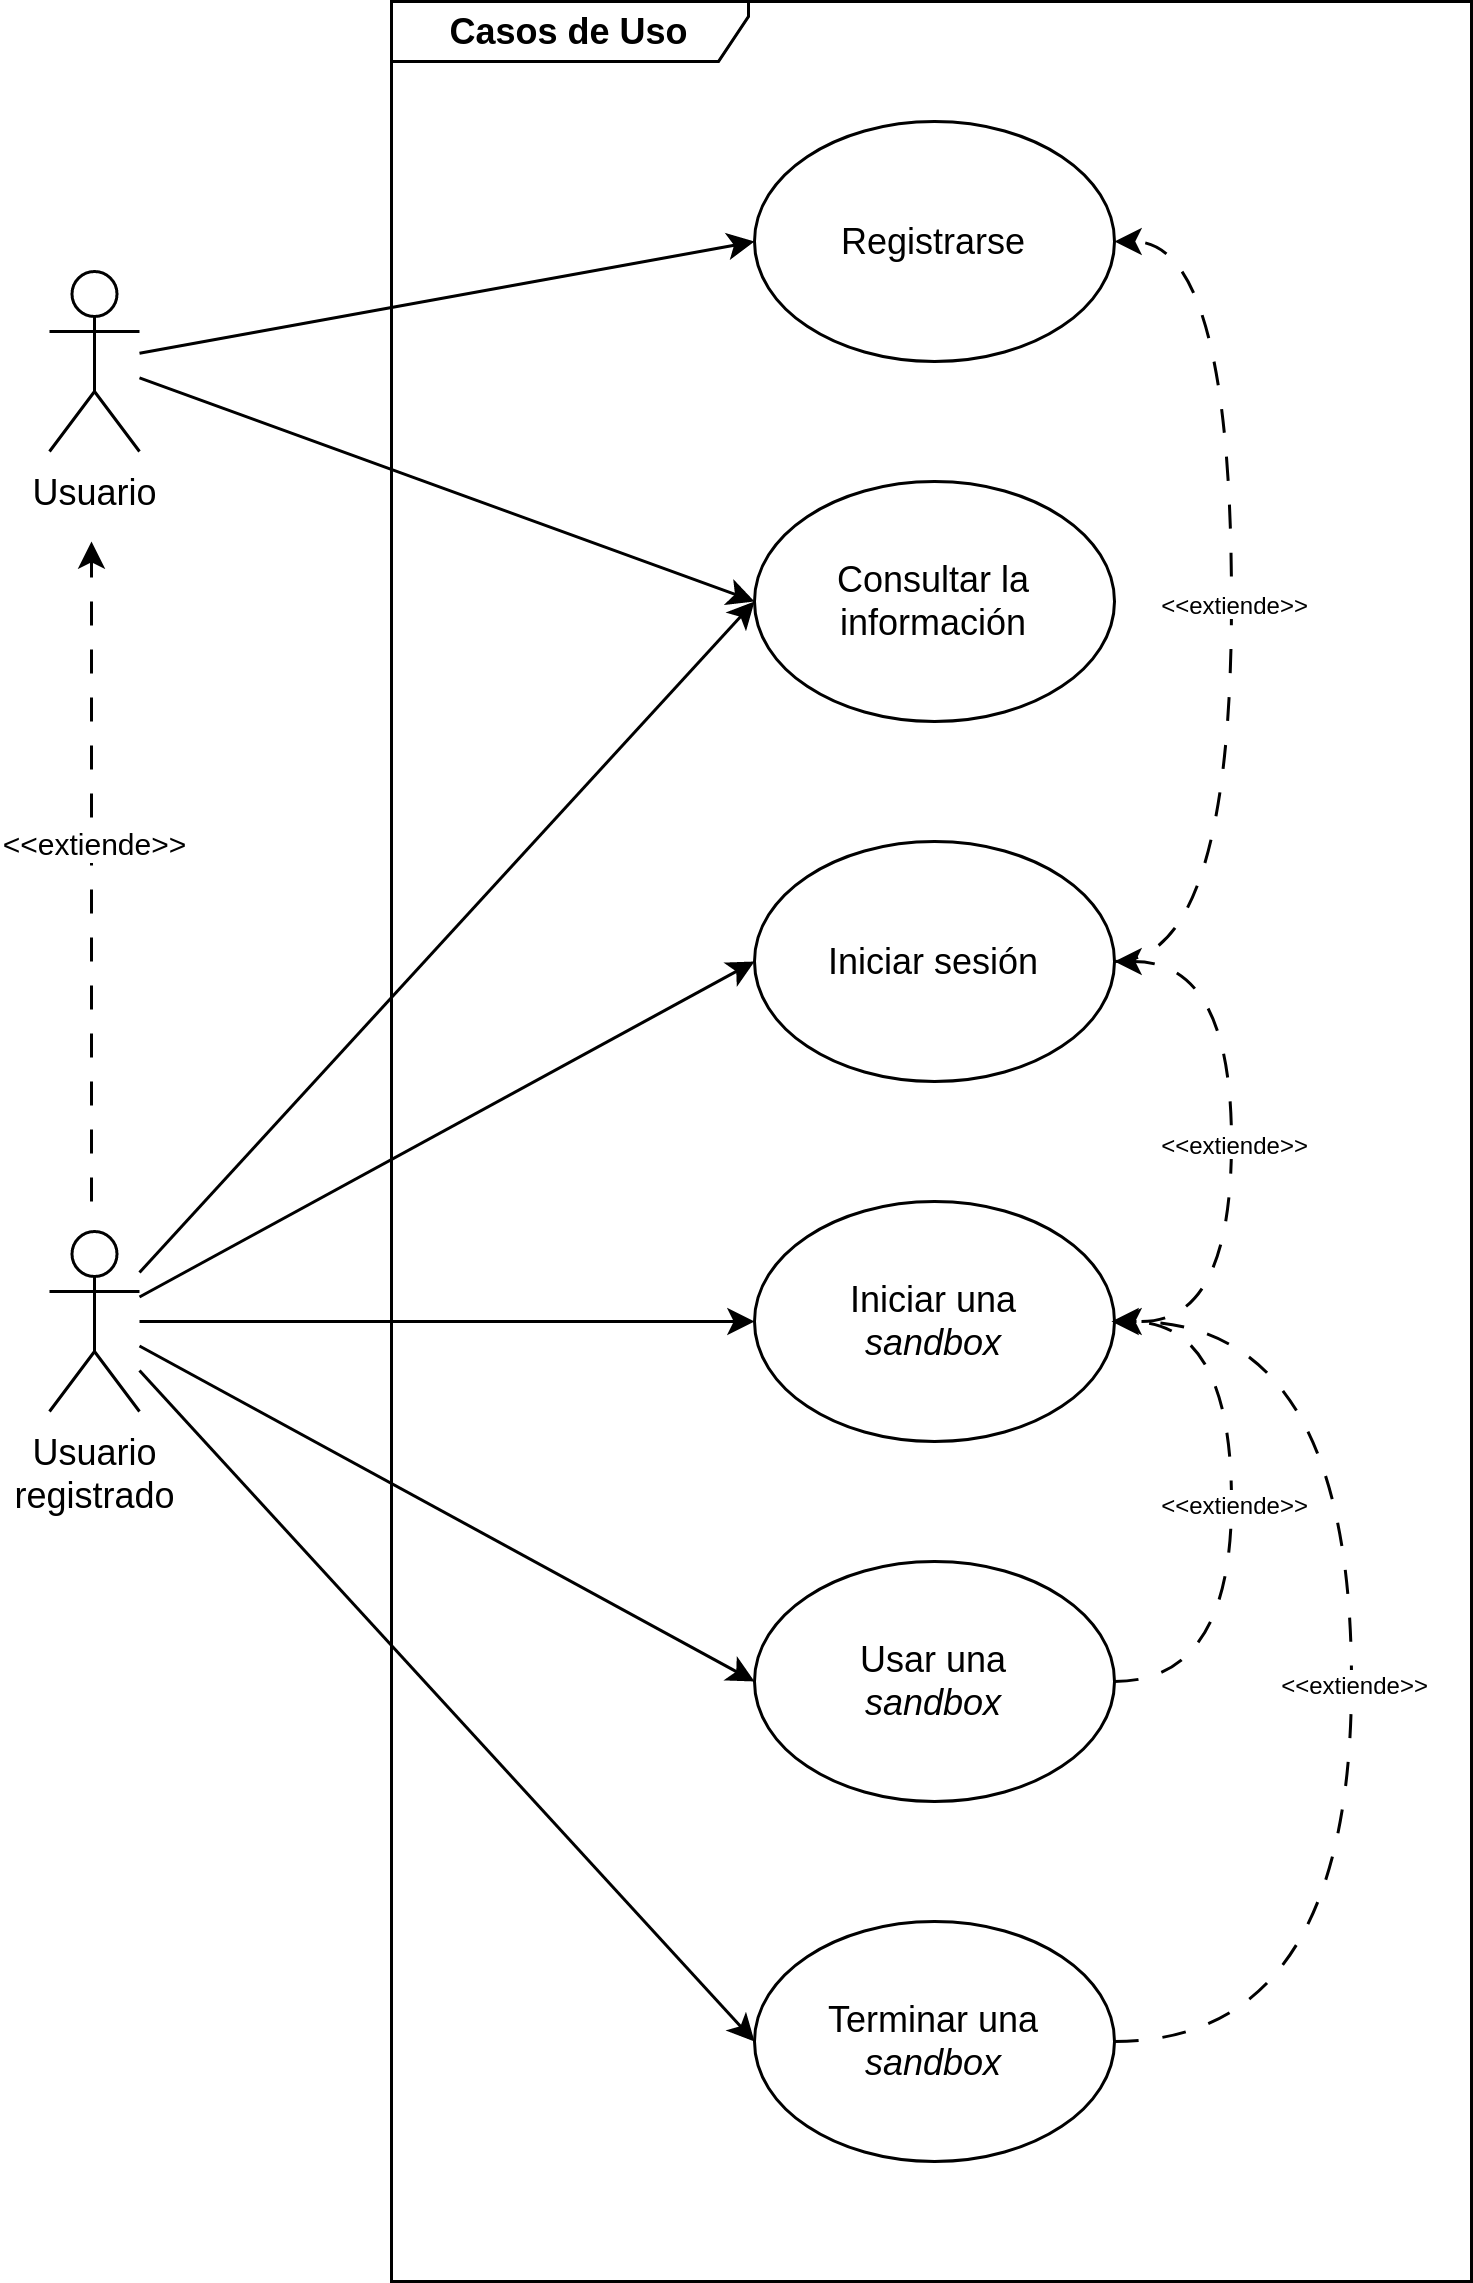
\includegraphics[scale=0.125]{images/Diagramas/Casos de uso.png}
                \caption{Casos de uso}
                \label{fig:casos-uso}
            \end{figure}
            
            \newpage
        
        
        \subsection{Requisitos funcionales}
            \label{sec:requisitos-funcionales}
            
            Los casos de uso permiten identificar los requisitos funcionales necesarios para satisfacer las necesidades del usuario y asegurarse de que el sistema cumpla con sus objetivos y expectativas. Teniendo eso en cuenta, los casos de uso describen cómo interactúan los usuarios con el sistema y qué acciones o funcionalidades deben estar disponibles en cada situación.
            
            Para este proyecto, se han definido los siguientes requisitos en función de los casos de uso mencionados en la sección anterior \ref{sec:casos-uso}:
            
            
            \subsubsection{Usuarios}
            
                Requisitos relacionados con la gestión de usuarios y sus datos.
                
                \begin{table}[!htbp]
                    \centering
                    \begin{tabular}{|c|c|}
                        \hline
                        \textbf{RF - 01} & \textbf{Registro de usuarios} \\
                        \hline
                        \multicolumn{2}{|p{15cm}|}{
                            El sistema debe permitir que los usuarios se registren y creen una cuenta en la plataforma para poder usar las \textit{sandboxes}.
                        } \\
                        \hline
                        \multicolumn{2}{|p{15cm}|}{
                            \begin{itemize}
                                \item Nombre de usuario.
                                \item Dirección de correo electrónico.
                                \item Contraseña.
                            \end{itemize}
                            } \\
                        \hline
                    \end{tabular}
                    \label{tab:RF1}
                \end{table}
                
                \begin{table}[!htbp]
                    \centering
                    \begin{tabular}{|c|c|}
                        \hline
                        \textbf{RF - 02} & \textbf{Inicio de sesión} \\
                        \hline
                        \multicolumn{2}{|p{15cm}|}{
                            El sistema debe permitir que los usuarios registrados puedan iniciar sesión para poder acceder al uso de las \textit{sandboxes}.
                        } \\
                        \hline
                    \end{tabular}
                    \label{tab:RF2}
                \end{table}
                
                \begin{table}[!htbp]
                    \centering
                    \begin{tabular}{|c|c|}
                        \hline
                        \textbf{RF - 03} & \textbf{Validación de los datos de registro} \\
                        \hline
                        \multicolumn{2}{|p{15cm}|}{
                            El sistema debe comprobar que los datos de registro de un usuario sean válidos.
                        } \\
                        \hline
                        \multicolumn{2}{|p{15cm}|}{
                            \begin{itemize}
                                \item No se registró un usuario con el mismo nombre de usuario ni correo electrónico.
                                \item Si alguno de los datos no es válido (error), se informará al usuario.
                            \end{itemize}
                            } \\
                        \hline
                    \end{tabular}
                    \label{tab:RF3}
                \end{table}
            
            
            \subsubsection{Contenido}
            
                Requisitos relacionados con la gestión de contenido y sus características.
                
                \begin{table}[!htbp]
                    \centering
                    \begin{tabular}{|c|c|}
                        \hline
                        \textbf{RF - 04} & \textbf{Consulta de contenido} \\
                        \hline
                        \multicolumn{2}{|p{15cm}|}{
                            El sistema debe proporcionar contenido relevante que permita a los usuarios adquirir los conocimientos necesarios para realizar las pruebas.
                        } \\
                        \hline
                    \end{tabular}
                    \label{tab:RF4}
                \end{table}
                
                \newpage
            
            
            \subsubsection{\textit{Sandboxes}}
            
                Requisitos relacionados con la gestión de los entornos virtualizados.
                
                \begin{table}[!htbp]
                    \centering
                    \begin{tabular}{|c|c|}
                        \hline
                        \textbf{RF - 05} & \textbf{Creación de \textit{sandboxes}} \\
                        \hline
                        \multicolumn{2}{|p{15cm}|}{
                            El sistema debe permitir que los usuarios seleccionen e inicien un laboratorio de pruebas que deseen realizar.
                        } \\
                        \hline
                        \multicolumn{2}{|p{15cm}|}{
                            \begin{itemize}
                                \item Si no es posible iniciar un laboratorio (error), se informará al usuario.
                            \end{itemize}
                            } \\
                        \hline
                    \end{tabular}
                    \label{tab:RF5}
                \end{table}
                
                \begin{table}[!htbp]
                    \centering
                    \begin{tabular}{|c|c|}
                        \hline
                        \textbf{RF - 06} & \textbf{Tiempo de vida de las \textit{sandboxes}} \\
                        \hline
                        \multicolumn{2}{|p{15cm}|}{
                            El sistema debe destruir automáticamente un laboratorio iniciado una vez que se haya superado un tiempo de vida definido.
                        } \\
                        \hline
                        \multicolumn{2}{|p{15cm}|}{
                            \begin{itemize}
                                \item Definir un tiempo de vida fijo para las \textit{sandboxes}.
                            \end{itemize}
                            } \\
                        \hline
                    \end{tabular}
                    \label{tab:RF6}
                \end{table}
                
                \begin{table}[!htbp]
                    \centering
                    \begin{tabular}{|c|c|}
                        \hline
                        \textbf{RF - 07} & \textbf{Número máximo de \textit{sandboxes} iniciadas} \\
                        \hline
                        \multicolumn{2}{|p{15cm}|}{
                            El sistema no debe permitir el inicio de infinitos laboratorios.
                        } \\
                        \hline
                        \multicolumn{2}{|p{15cm}|}{
                            \begin{itemize}
                                \item Definir un número máximo de instancias posibles.
                            \end{itemize}
                            } \\
                        \hline
                    \end{tabular}
                    \label{tab:RF7}
                \end{table}
                
                \begin{table}[!htbp]
                    \centering
                    \begin{tabular}{|c|c|}
                        \hline
                        \textbf{RF - 08} & \textbf{Uso de una \textit{sandbox} iniciada} \\
                        \hline
                        \multicolumn{2}{|p{15cm}|}{
                            El sistema debe permitir que los usuarios puedan conectarse a un laboratorio una vez este se haya iniciado.
                        } \\
                        \hline
                        \multicolumn{2}{|p{15cm}|}{
                            \begin{itemize}
                                \item Proporcionar los datos de conexión a un laboratorio al usuario.
                                \item La conexión se realizará por el propio usuario a través de SSH.
                            \end{itemize}
                            } \\
                        \hline
                    \end{tabular}
                    \label{tab:RF8}
                \end{table}
                
                \begin{table}[!htbp]
                    \centering
                    \begin{tabular}{|c|c|}
                        \hline
                        \textbf{RF - 09} & \textbf{Destrucción de \textit{sandboxes}} \\
                        \hline
                        \multicolumn{2}{|p{15cm}|}{
                            El sistema debe permitir que los usuarios puedan apagar una \textit{sandbox}, lo que equivale a destruirla manualmente (en lugar de esperar a que se cumpla su tiempo de vida).
                        } \\
                        \hline
                        \multicolumn{2}{|p{15cm}|}{
                            \begin{itemize}
                                \item Si no es posible destruir un laboratorio (error), se informará al usuario.
                                \item Un administrador podrá acceder a registros de uso de los laboratorios.
                            \end{itemize}
                            } \\
                        \hline
                    \end{tabular}
                    \label{tab:RF09}
                \end{table}
                
                \newpage
        
        
        \subsection{Requisitos no funcionales}
            \label{sec:requisitos-nofuncionales}
            
            Por otro lado, los requisitos no funcionales describen las cualidades o atributos que debe tener un sistema, enfocándose en cómo hace el sistema lo que hace; es decir, cómo se comporta en términos de calidad.
            
            Para este proyecto, se han definido los siguientes requisitos en función de los requisitos mencionados en la sección anterior \ref{sec:requisitos-funcionales} y los objetivos de la plataforma:
            
            \begin{table}[!htbp]
                \centering
                \begin{tabular}{|c|c|}
                    \hline
                    \textbf{RNF - 01} & \textbf{Privacidad de los datos} \\
                    \hline
                    \multicolumn{2}{|p{15cm}|}{
                        El sistema debe garantizar la seguridad y privacidad de los datos de los usuarios.
                    } \\
                    \hline
                    \multicolumn{2}{|p{15cm}|}{
                        \begin{itemize}
                            \item Aplicar una política de cifrado para las contraseñas.
                        \end{itemize}
                        } \\
                    \hline
                \end{tabular}
                \label{tab:RNF1}
            \end{table}
            
            \begin{table}[!htbp]
                \centering
                \begin{tabular}{|c|c|}
                    \hline
                    \textbf{RNF - 02} & \textbf{Aislamiento de las \textit{sandboxes}} \\
                    \hline
                    \multicolumn{2}{|p{15cm}|}{
                        El sistema debe garantizar la seguridad y aislamiento de los laboratorios de prueba de la plataforma.
                    } \\
                    \hline
                    \multicolumn{2}{|p{15cm}|}{
                        \begin{itemize}
                            \item Aislar completamente los laboratorios sin afectar al resto de la plataforma.
                        \end{itemize}
                        } \\
                    \hline
                \end{tabular}
                \label{tab:RNF2}
            \end{table}
            
            \begin{table}[!htbp]
                \centering
                \begin{tabular}{|c|c|}
                    \hline
                    \textbf{RNF - 03} & \textbf{Seguridad de la plataforma} \\
                    \hline
                    \multicolumn{2}{|p{15cm}|}{
                        El sistema debe implementar medidas de seguridad para prevenir ataques externos o internos a la plataforma.
                    } \\
                    \hline
                    \multicolumn{2}{|p{15cm}|}{
                        \begin{itemize}
                            \item Medidas de autenticación y autorización para garantizar el acceso solo a usuarios autorizados.
                        \end{itemize}
                        } \\
                    \hline
                \end{tabular}
                \label{tab:RNF3}
            \end{table}
            
            \begin{table}[!htbp]
                \centering
                \begin{tabular}{|c|c|}
                    \hline
                    \textbf{RNF - 04} & \textbf{Accesibilidad} \\
                    \hline
                    \multicolumn{2}{|p{15cm}|}{
                        La plataforma debe ser accesible para cualquier usuario, independientemente de su nivel de experiencia en ciberseguridad.
                    } \\
                    \hline
                    \multicolumn{2}{|p{15cm}|}{
                        \begin{itemize}
                            \item Contenido claro y accesible.
                            \item Laboratorios bien estructurados.
                        \end{itemize}
                        } \\
                    \hline
                \end{tabular}
                \label{tab:RNF4}
            \end{table}
            
            \begin{table}[!htbp]
                \centering
                \begin{tabular}{|c|c|}
                    \hline
                    \textbf{RNF - 05} & \textbf{Usabilidad} \\
                    \hline
                    \multicolumn{2}{|p{15cm}|}{
                        La plataforma debe ser fácil de usar y accesible para cualquier usuario, independientemente de su nivel de experiencia en ciberseguridad.
                    } \\
                    \hline
                    \multicolumn{2}{|p{15cm}|}{
                        \begin{itemize}
                            \item Interfaz de usuario intuitiva, clara y organizada.
                        \end{itemize}
                        } \\
                    \hline
                \end{tabular}
                \label{tab:RNF5}
            \end{table}
            
            \begin{table}[H]
                \centering
                \begin{tabular}{|c|c|}
                    \hline
                    \textbf{RNF - 06} & \textbf{Extensibilidad} \\
                    \hline
                    \multicolumn{2}{|p{15cm}|}{
                        La plataforma debe ser fácilmente extensible, permitiendo la futura integración de más contenido y laboratorios de pruebas.
                    } \\
                    \hline
                    \multicolumn{2}{|p{15cm}|}{
                        \begin{itemize}
                            \item Definir y documentar claramente cómo añadir contenido y laboratorios.
                        \end{itemize}
                        } \\
                    \hline
                \end{tabular}
                \label{tab:RNF6}
            \end{table}
            
            \cleardoublepage
    
    
    \section{Arquitectura}
        \label{sec:arquitectura}
        
        \begin{figure}[h]
            \centering
            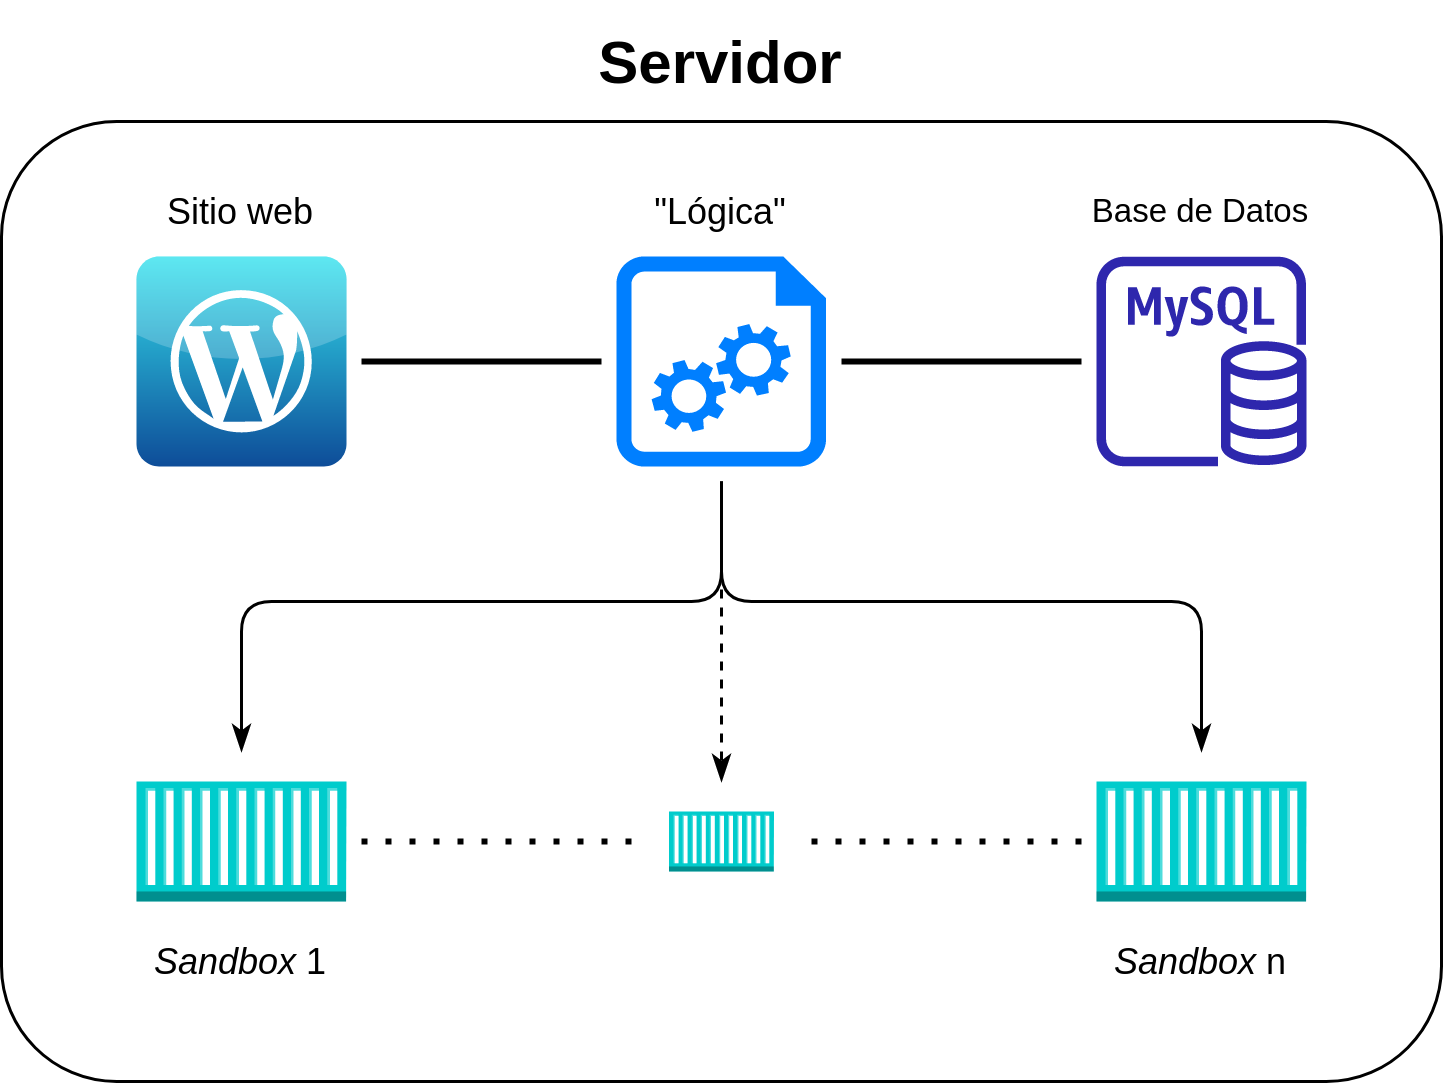
\includegraphics[scale=0.20]{images/Diagramas/Arquitectura.png}
            \caption{Arquitectura}
            \label{fig:arquitectura}
        \end{figure}

        Los componentes de la plataforma podrían dividirse en 4 partes fundamentales: el front-end, el back-end, la base de datos y los contenedores Docker (laboratorios). Todos estos están desplegados en un servidor que utiliza LAMP.

        \subsection{\textit{Front-end}: WordPress}

            El front-end es la parte de la plataforma que interactúa con el usuario. En este caso, se ha desarrollado una aplicación web que permite al usuario acceder a la plataforma y realizar las acciones que se describen en la sección \ref{sec:casos-uso}.
            
            Esta plataforma web se ha desarrollado utilizando el gestor de contenidos WordPress, ya que permite crear sitios web de forma rápida y sencilla, sin necesidad de tener conocimientos avanzados de programación. Además, cuenta con una gran comunidad de desarrolladores que crean y mantienen plugins y temas para extender las funcionalidades de la plataforma.


        \subsection{\textit{Back-end}: \texttt{functions.php}}
        
            El back-end es la parte de la plataforma que se encarga de procesar las peticiones del usuario y de gestionar los recursos de la plataforma. En este caso, se encarga de gestionar las peticiones del usuario y de comunicarse con la base de datos y los contenedores Docker.
            
            Se ha usado el fichero \textit{functions.php} de WordPress para implementar el back-end de la plataforma, ya que permite extender las funcionalidades de WordPress de forma sencilla. Se ejecuta en cada petición que se realiza a la plataforma, por lo que se ha usado para implementar las funcionalidades necesarias para la gestión y configuración de los laboratorios de pruebas ejecutados por los usuarios.

            Además, se ha añadido una tarea de cron con la que comprobar si algún laboratorio de pruebas superó su tiempo de vida (1 hora). Esta tarea se ejecuta cada minuto y destruye dichos laboratorios, liberando recursos en el sistema.


        \subsection{Base de datos: MySQL}

            La base de datos es la parte de la plataforma que se encarga de almacenar la información de los usuarios y de los laboratorios de pruebas. En este caso, se ha usado para almacenar la información de los usuarios registrados en la plataforma y de los laboratorios de pruebas que han sido creados por dichos usuarios.
            
            Se ha usado MySQL como gestor de base de datos, ya que es un sistema de gestión de bases de datos relacional, de código abierto y muy popular. Además, es compatible con WordPress, por lo que se puede acceder a la base de datos desde el fichero \textit{functions.php}.
        
        
        \subsection{Contenedores Docker: laboratorios de pruebas}

            Los contenedores Docker son la parte de la plataforma que se encarga de ejecutar los laboratorios de pruebas. En este caso, se ha usado para ejecutar los laboratorios de pruebas que han sido creados por los usuarios.
            
            Se ha usado Docker para ejecutar los laboratorios de pruebas, ya que permite ejecutar aplicaciones en contenedores de software. Estos contenedores son ligeros y portables, por lo que se pueden ejecutar en cualquier máquina que tenga Docker instalado. Además, se pueden crear imágenes de los contenedores, lo que permite crear laboratorios de pruebas personalizados y compartirlos con otros usuarios.
            
        
        \subsection{Conexión a un laboratorio}
        
            \begin{figure}[h]
                \centering
                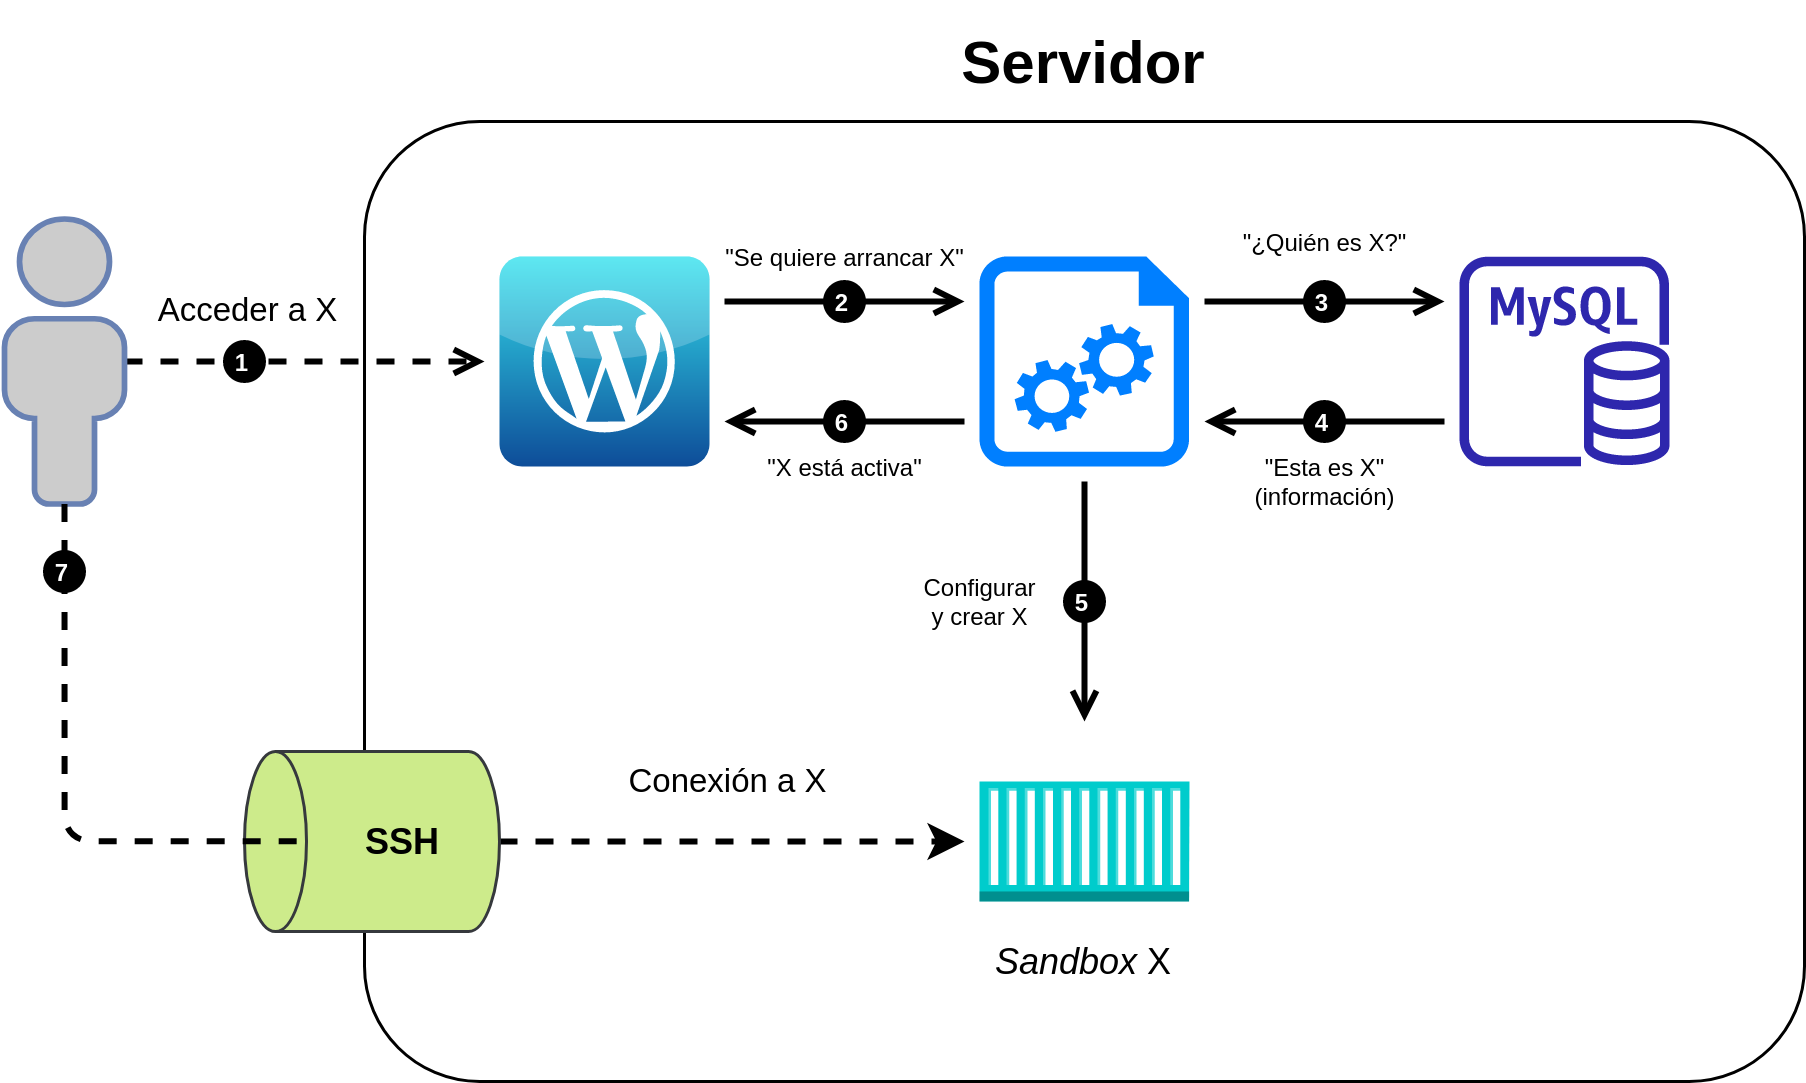
\includegraphics[scale=0.20]{images/Diagramas/Arquitectura 1.png}
                \caption{Uso normal}
                \label{fig:conexion-sandbox}
            \end{figure}
            
            El usuario está registrado, ya que en caso contrario, no podría acceder a esta funcionalidad del sistema.
            
            \begin{itemize}
                \item El usuario que ha accedido a la plataforma quiere encender un laboratorio.
                \item Se informa al servidor de dicha acción y se consulta en la base de datos la información de dicho entorno virtualizado (ID, nombre, características de construcción, tiempo de vida...).
                \item Una vez obtenido dicha información, se procesa y se inicia la construcción de una instancia del laboratorio.
                \item Finalmente, tras haberse construido el entorno, el usuario recibe un mensaje con los datos de conexión y puede proceder a conectarse al entorno a través de SSH.
            \end{itemize}
            
            \newpage
    
    
    \section{Modelado de actividades y transiciones}
        \label{sec:modelado-actividades-transiciones}

        Los diagramas mostrados a continuación presentan las actividades que puede realizar un usuario en la plataforma y las transiciones entre dichas actividades.
        
        Estos diagramas se han desarrollado utilizando la herramienta \textit{draw.io}.
        
        \subsection{Tratamiento de usuarios}
        
            \begin{figure}[h]
                \centering
                \begin{subfigure}{0.45\textwidth}
                    \centering
                    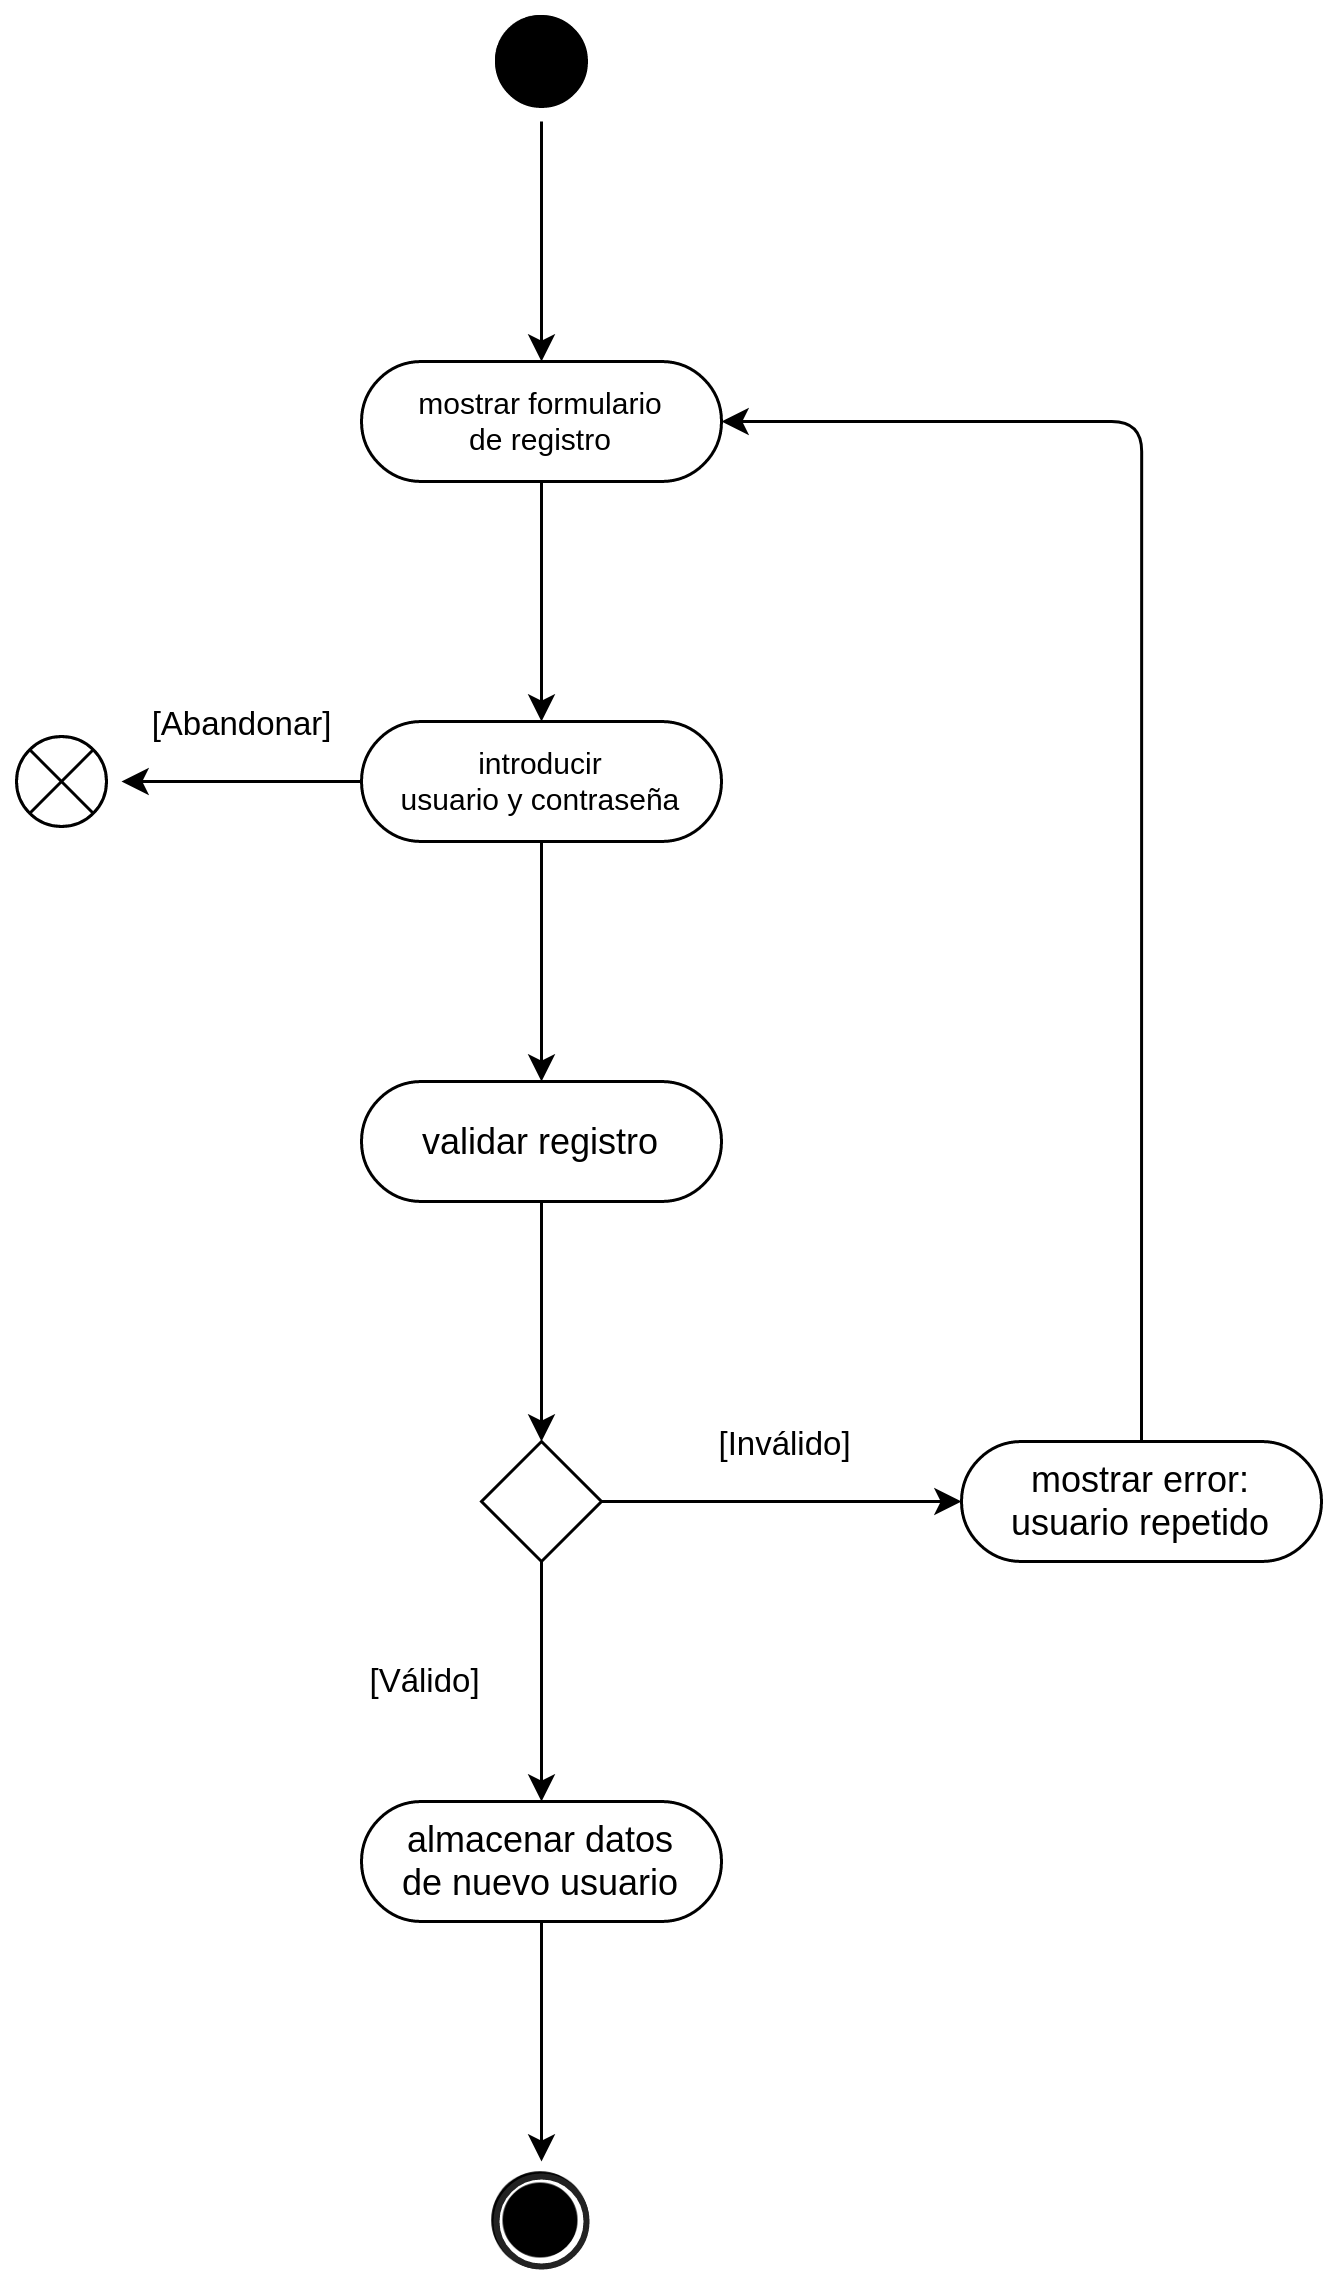
\includegraphics[scale=0.15]{images/Diagramas/Actividades y transiciones 1.png}
                    \caption{Registro de un usuario}
                    \label{fig:registro-usuario}
                \end{subfigure}
                \hfill
                \begin{subfigure}{0.45\textwidth}
                    \centering
                    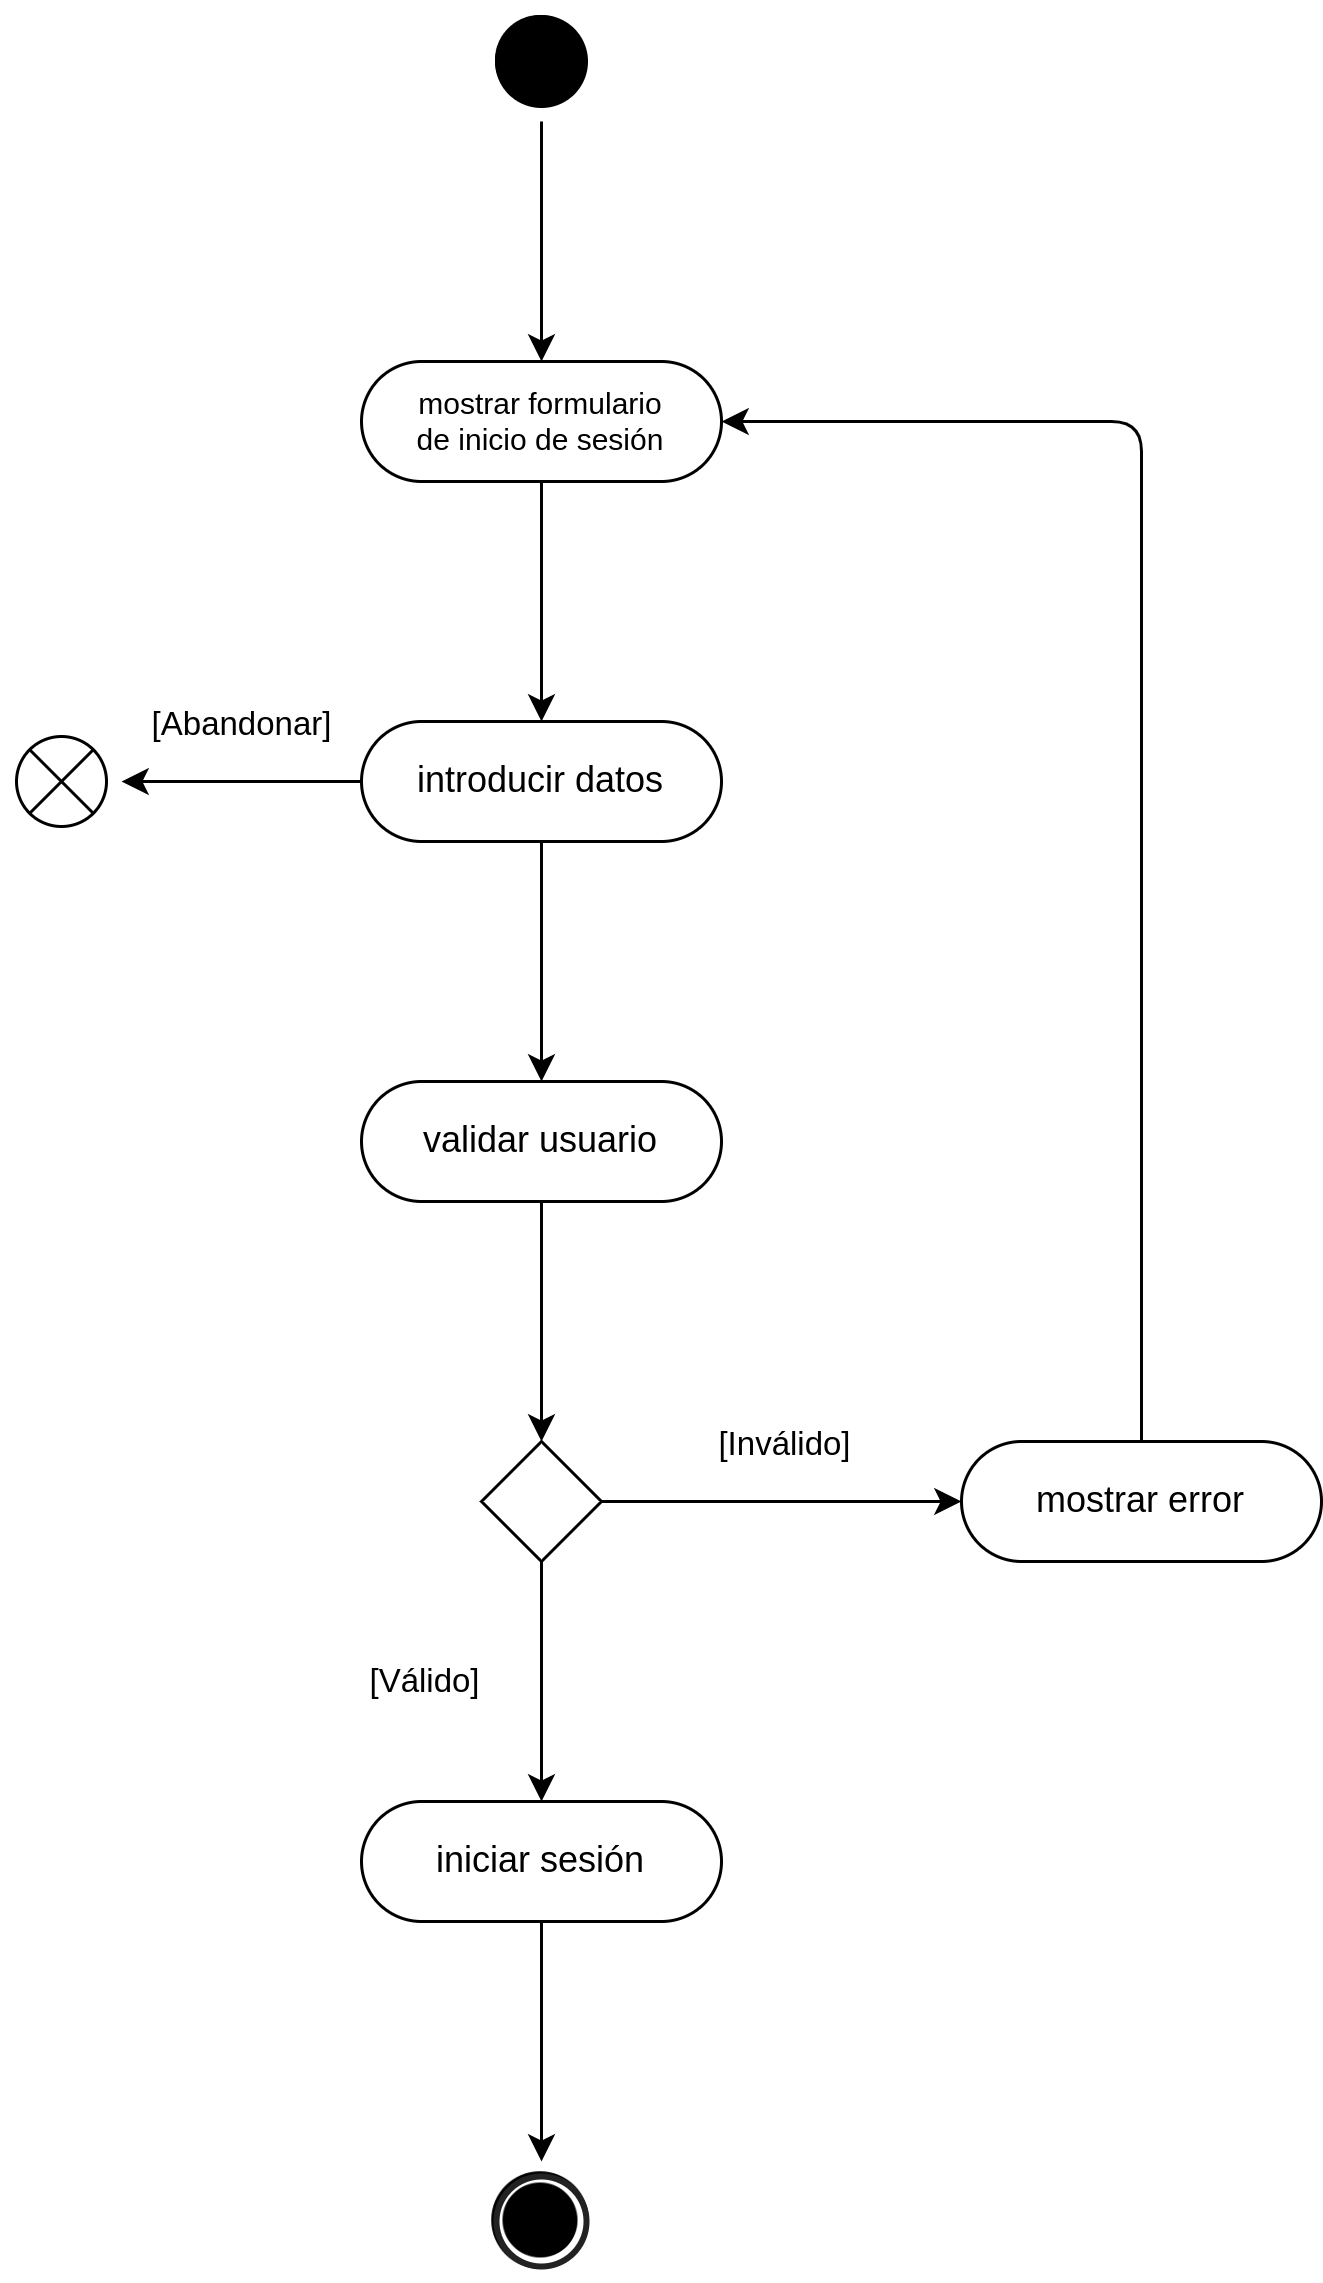
\includegraphics[scale=0.15]{images/Diagramas/Actividades y transiciones 2.png}
                    \caption{Inicio de sesión de un usuario}
                    \label{fig:inicio-usuario}
                \end{subfigure}
                \caption{Modelado de actividades y transiciones}
                \label{fig:tratamiento-usuarios}
            \end{figure}
            
            Los diagramas presentados en esta sección definen la gestión de usuarios que permite el registro e inicio de sesión de los mismos en la plataforma.
            
            El proceso de registro de un usuario mostrará inicialmente un formulario para poder obtener sus datos, debiendo verificar que dichos datos no pertenecen a un usario previamente registrado, puesto que los usuarios deben ser únicos.
            
            El proceso de inicio de sesión de un usuario mostrará un funcionamiento similar al de registro, pero esta vez, para comprobar que el usuario sí ha sido registrado anteriormente.
            
            \newpage
            
            
        \subsection{Consulta de la documentación}
            \label{sec:consulta-documentacion}
            
            \begin{figure}[h]
                \centering
                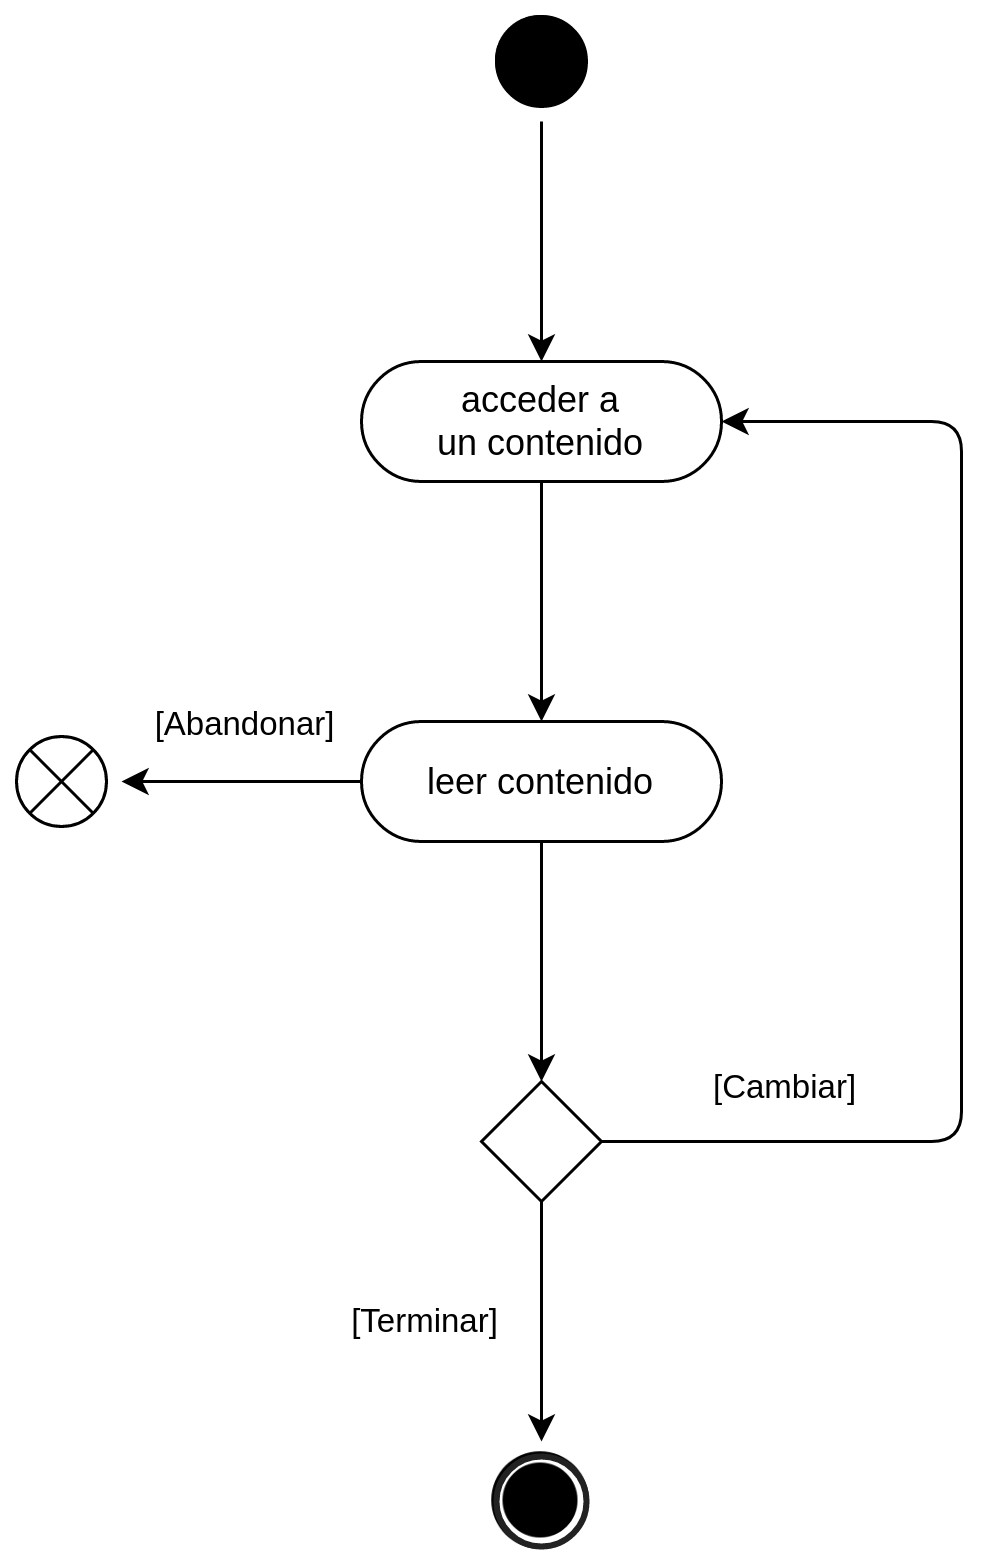
\includegraphics[scale=0.20]{images/Diagramas/Actividades y transiciones 3.png}
                \caption{Consulta de documentación}
                \label{fig:consulta-documentacion}
            \end{figure}
            
            El diagrama presentado en esta sección define el consumo de contenido de la plataforma por parte de un usuario, esté registrado o no, ya que el contenido instructivo de la plataforma se considera público, al contrario que el uso de los laboratorios que requerirá un registro por parte del usuario.
            
            El proceso de consulta de documentación es bastante simple: un usuario puede consumir contenido de forma continua, pero al estar dividido por conceptos, necesitará cambiar de ubicación dentro de la plataforma para poder seguir accediendo a contenido nuevo.
            
            \newpage
            
            
        \subsection{Tratamiento de laboratorios}
        
            \begin{figure}[h]
                \centering
                \begin{subfigure}{0.45\textwidth}
                    \centering
                    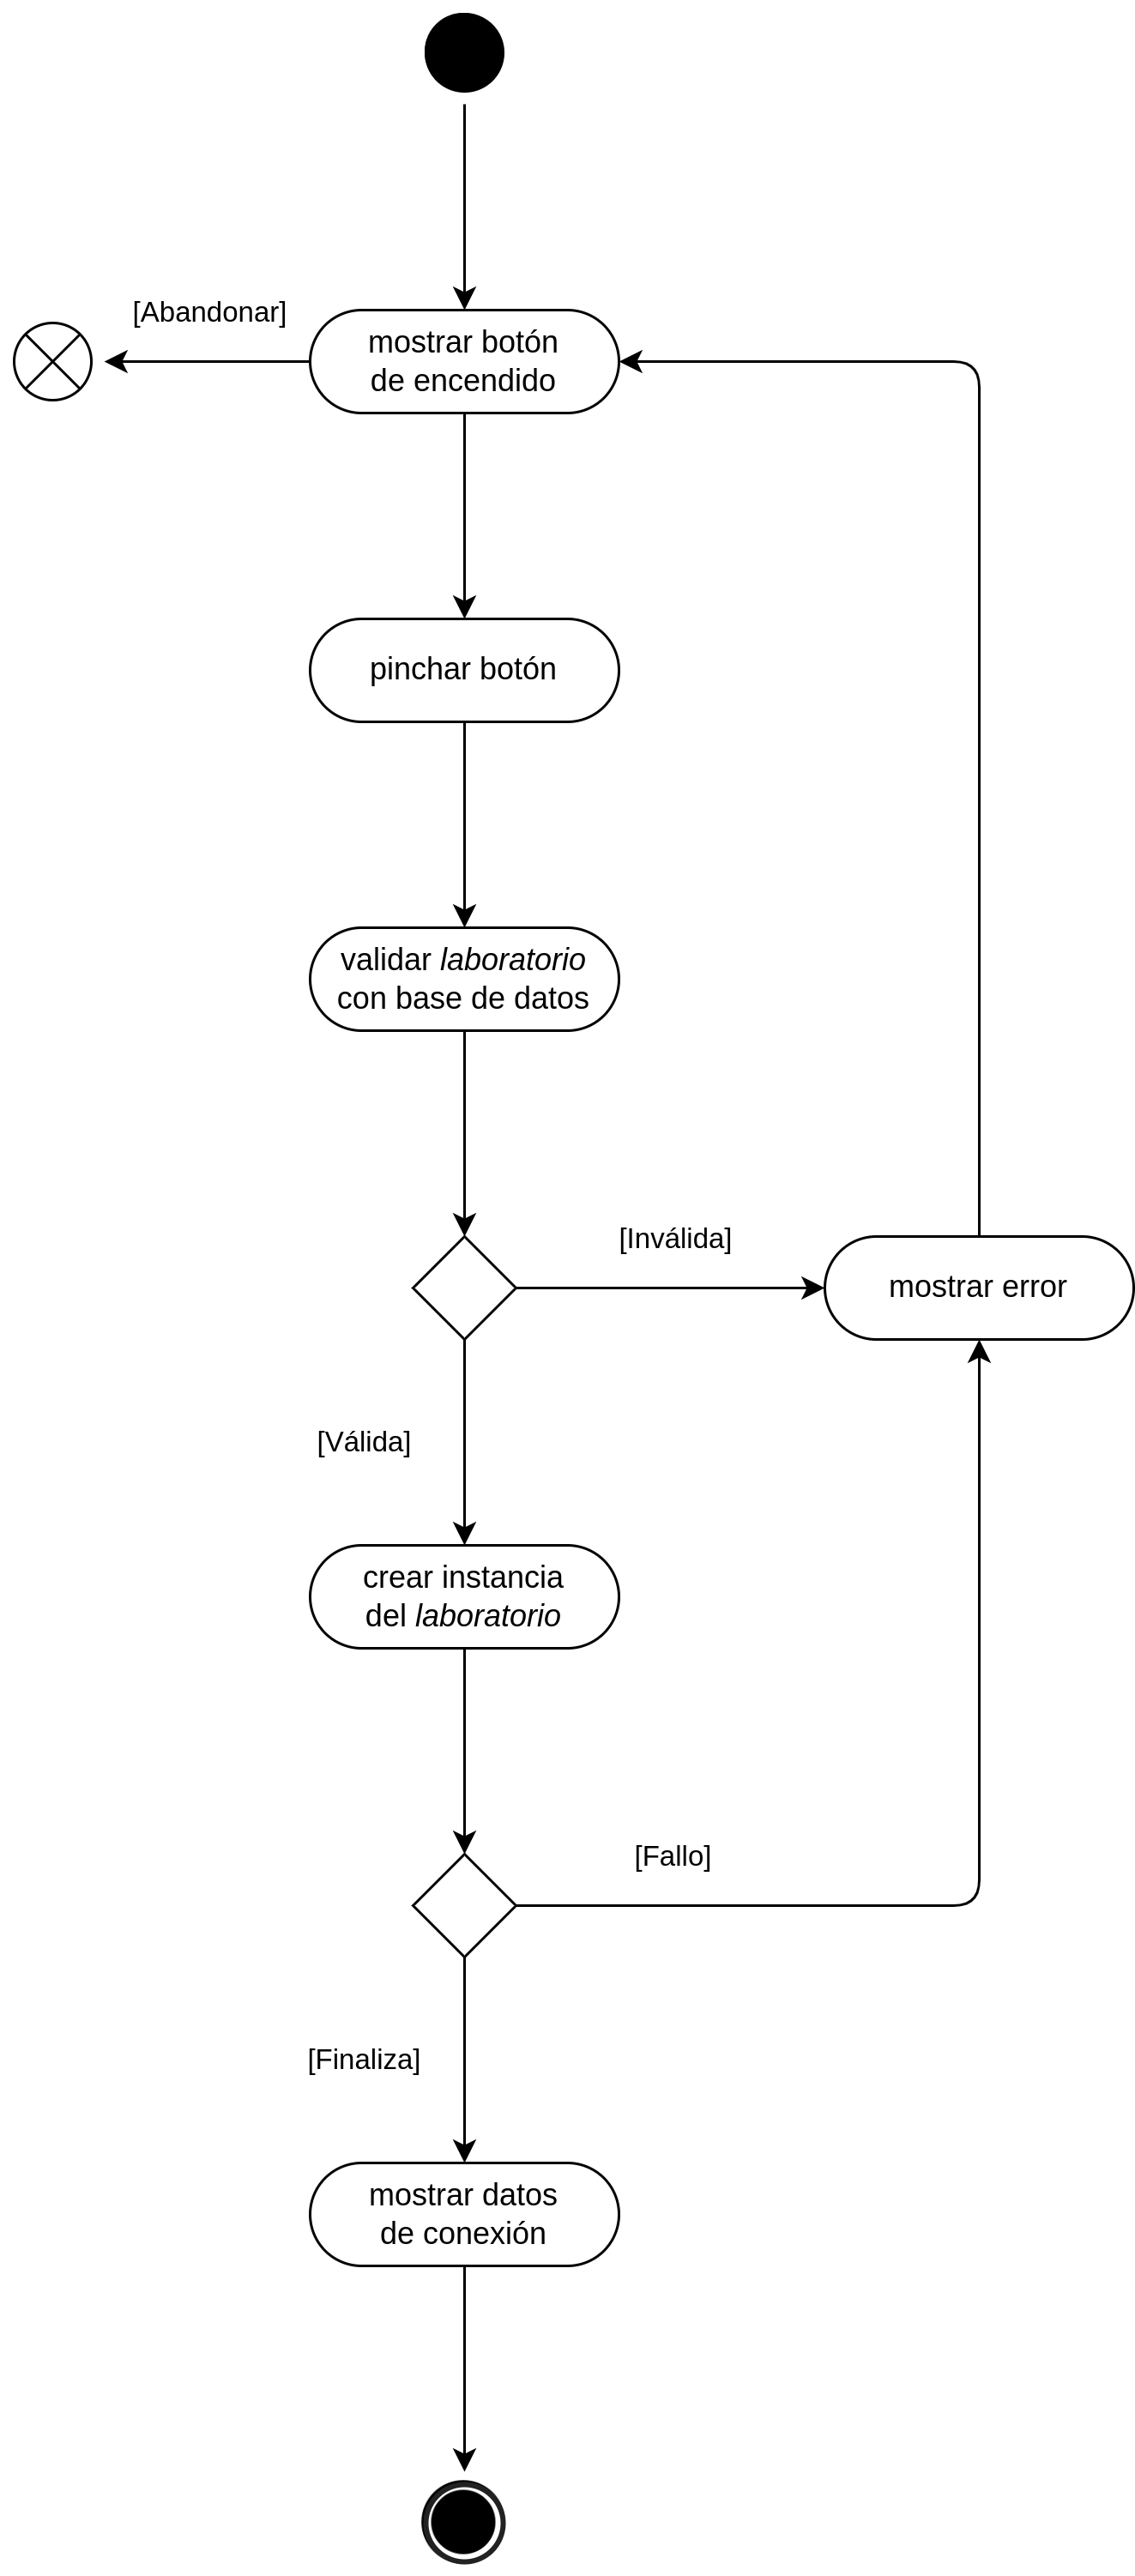
\includegraphics[scale=0.115]{images/Diagramas/Actividades y transiciones 4.png}
                    \caption{Creación de un laboratorio}
                    \label{fig:creacion-laboratorio}
                \end{subfigure}
                \hfill
                \begin{subfigure}{0.45\textwidth}
                    \centering
                    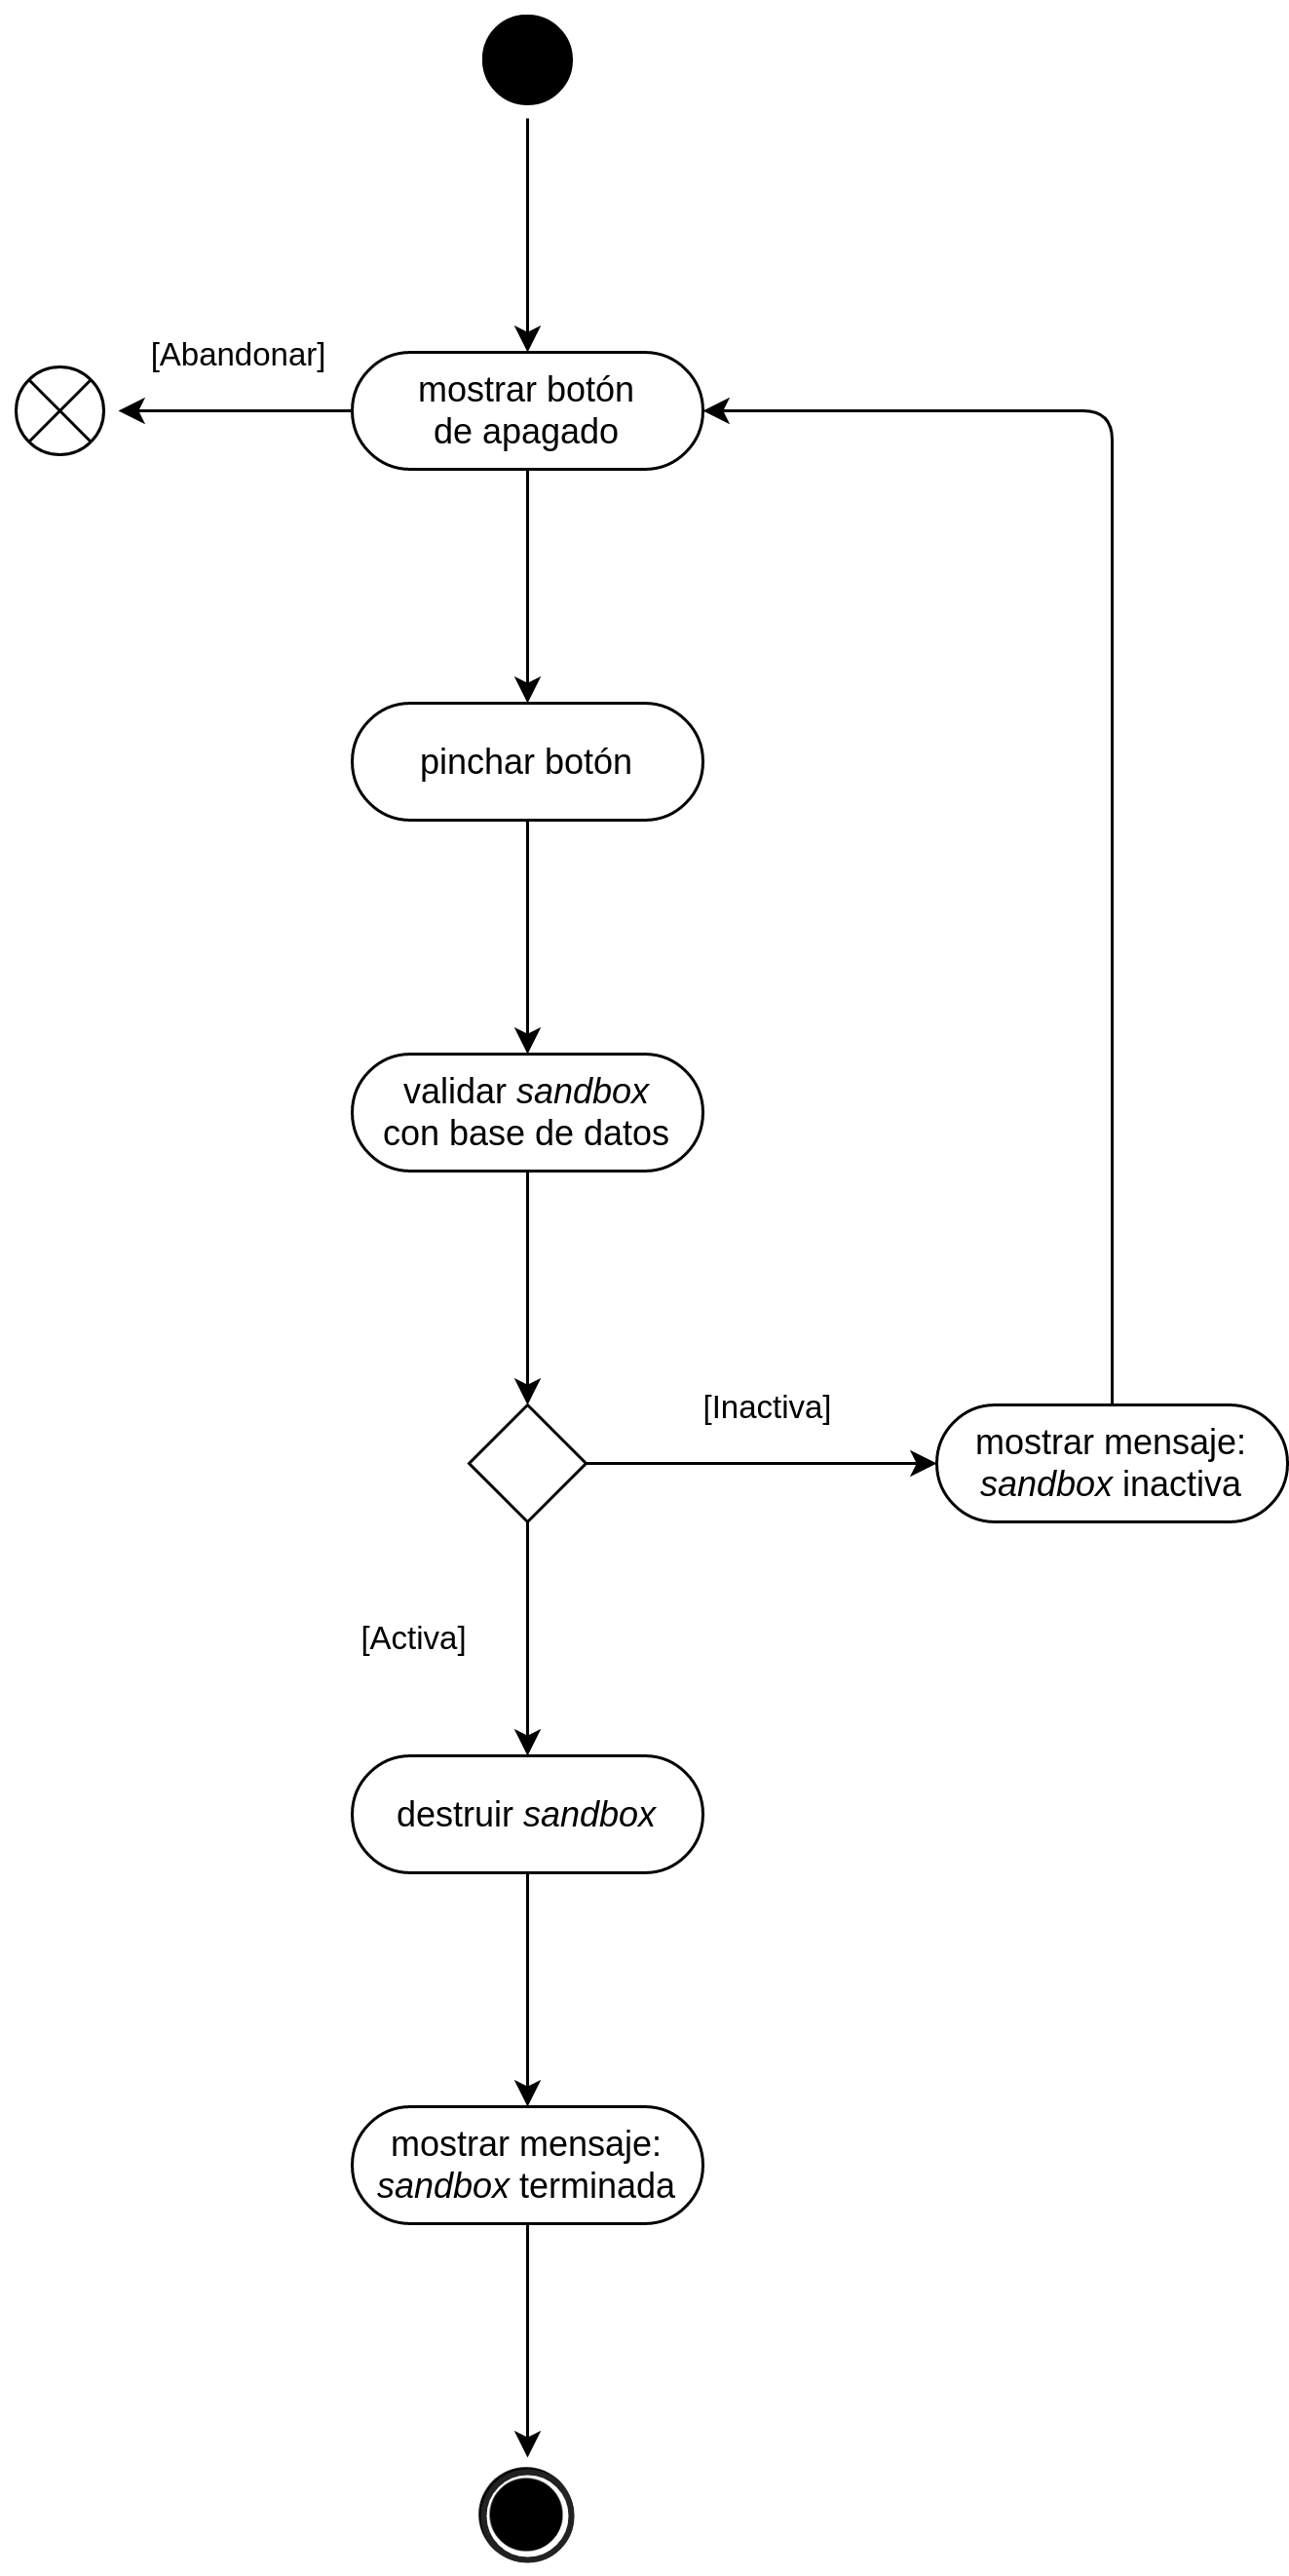
\includegraphics[scale=0.115]{images/Diagramas/Actividades y transiciones 5.png}
                    \caption{Destrucción de un laboratorio}
                    \label{fig:destruccion-laboratorio}
                \end{subfigure}
                \caption{Tratamiento de laboratorios}
                \label{fig:tratamiento-laboratorios}
            \end{figure}
            
            Los diagramas presentados en esta sección definen la gestión de entornos virtualizados de la plataforma.
            
            El proceso de creación de un laboratorio iniciará pulsando un botón, preferiblemente ubicado al final de un contenido instructivo descrito anteriormente en \textit{Consulta de la documentación} \ref{sec:consulta-documentacion}, debiendo verificar que es posible crear dicho laboratorio.
            
            El proceso de destrucción de un laboratorio seguirá el mismo proceso que el anterior, pero realizará la opción opuesta.

            \newpage


            \begin{figure}[h]
                \centering

                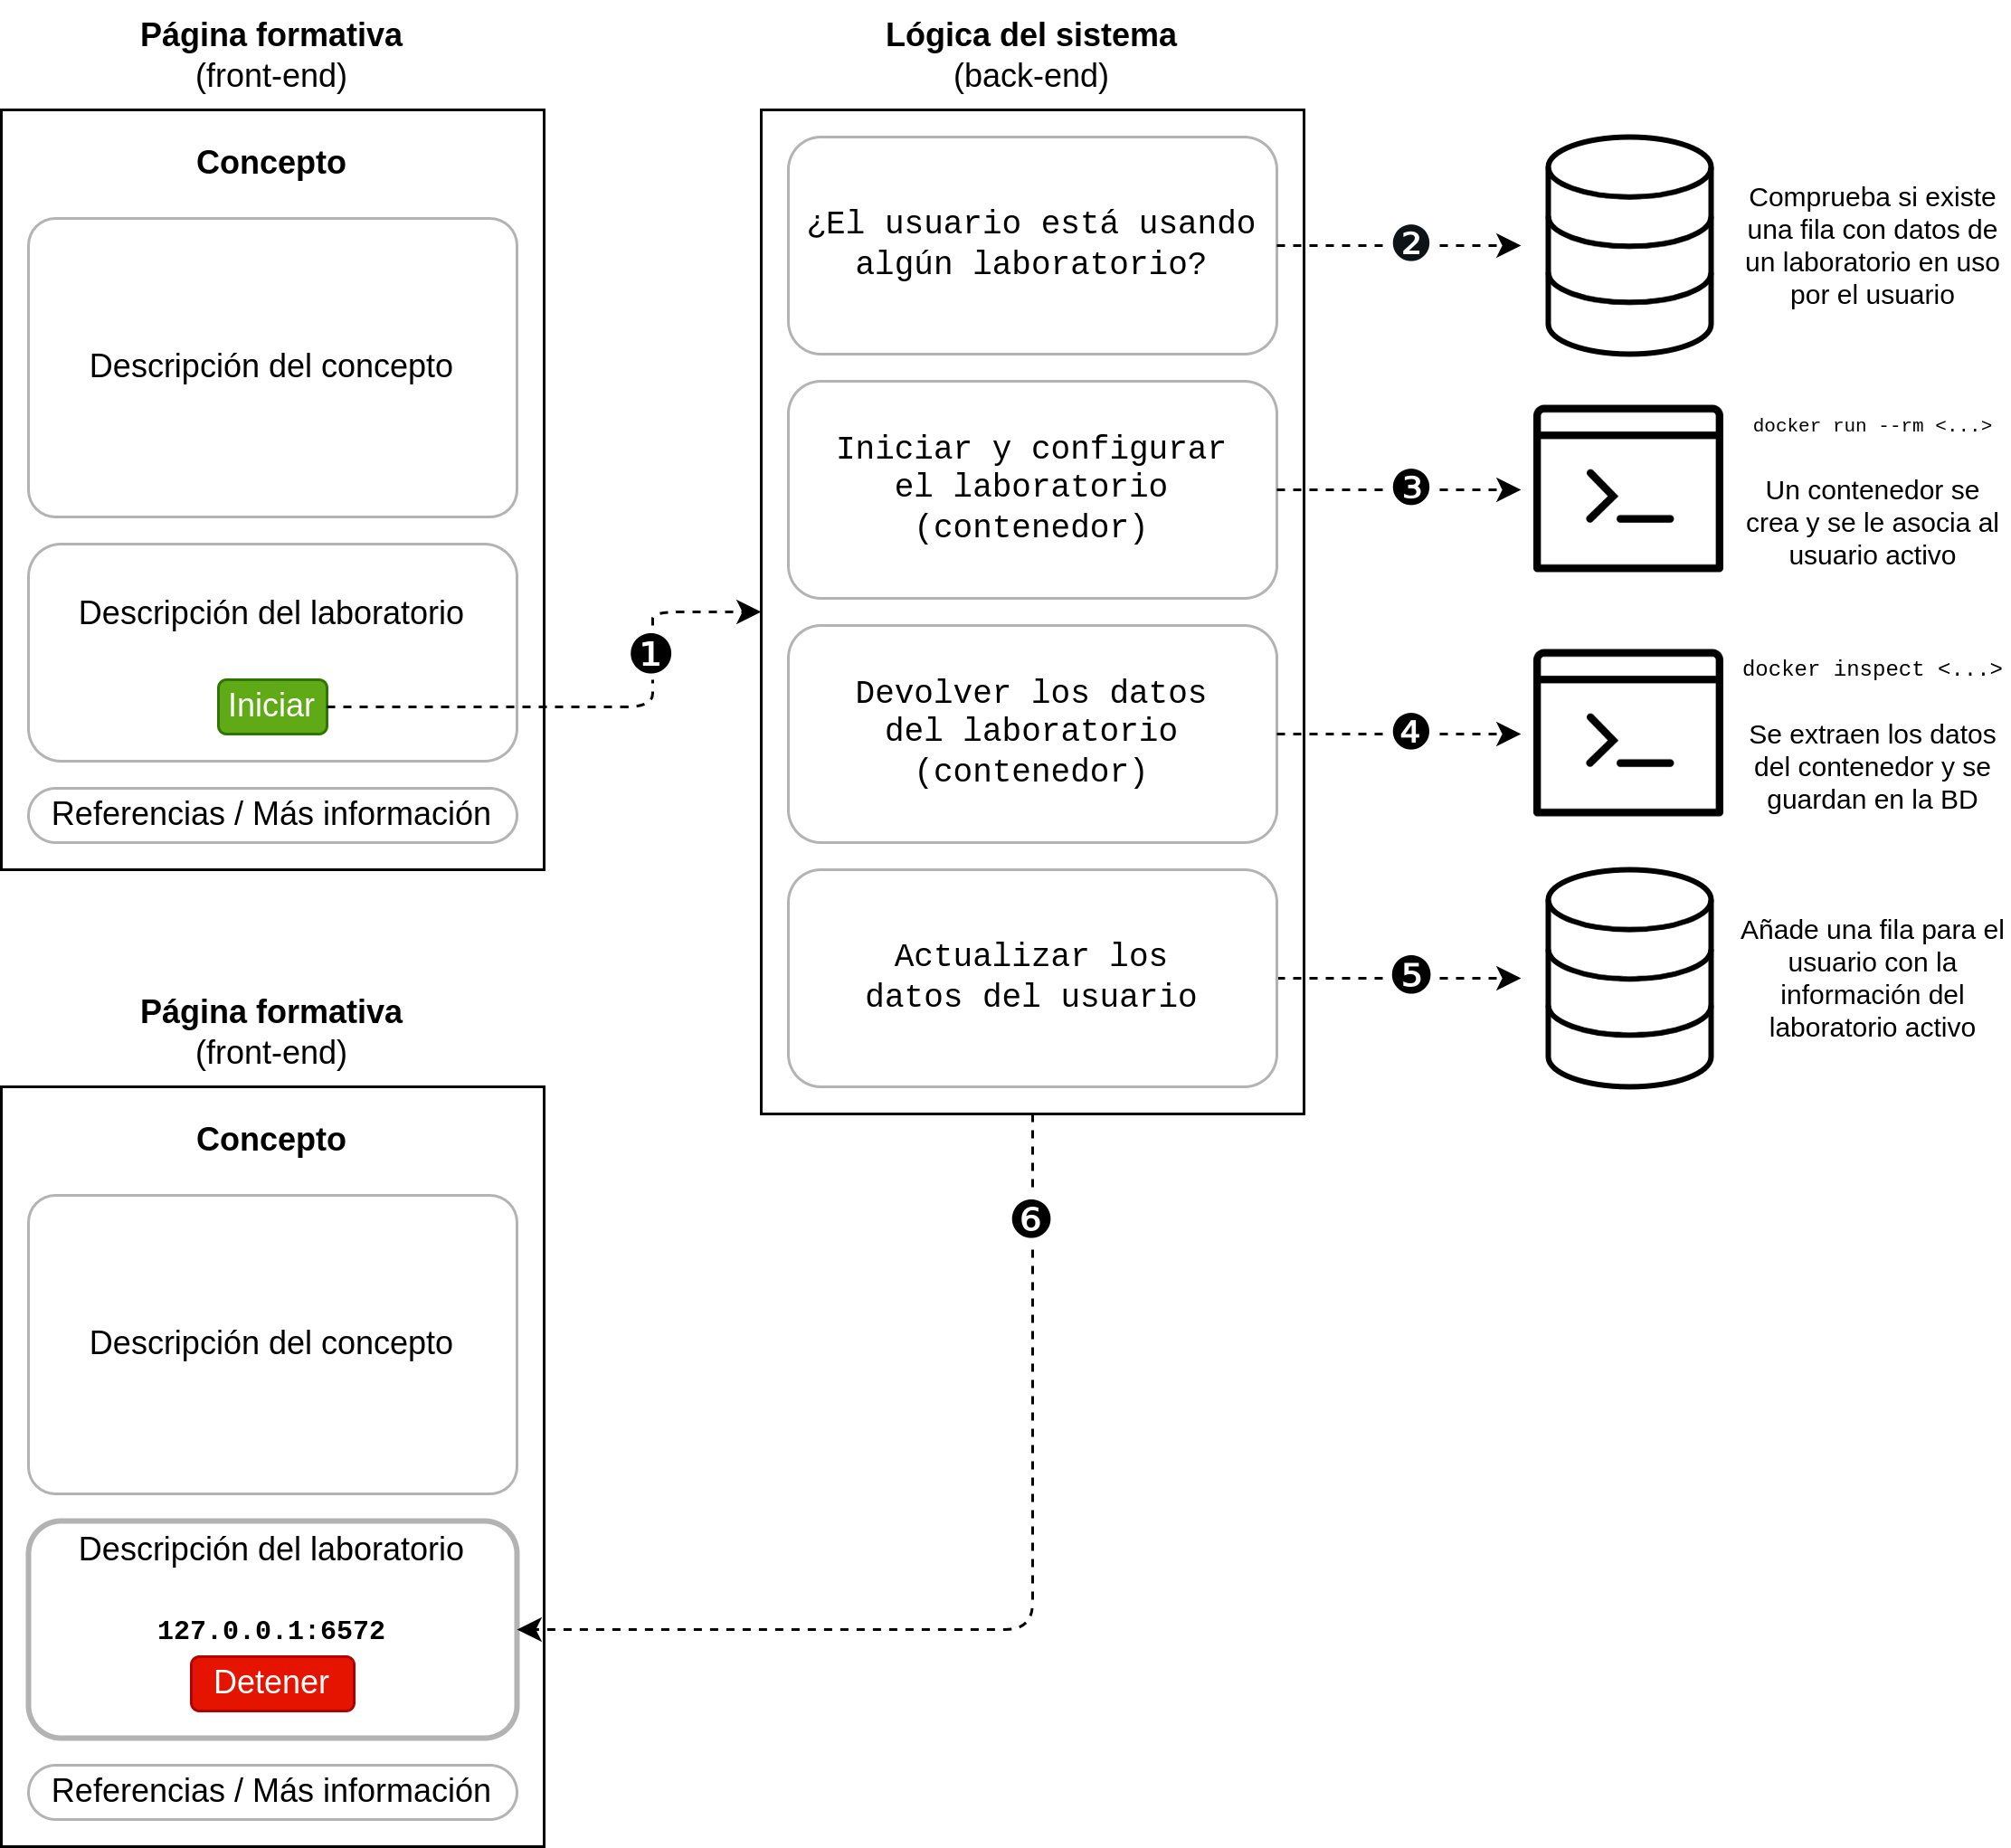
\includegraphics[scale=0.125]{images/Diagramas/iniciar.png}
                \caption{Inicio de un laboratorio desde el sitio web}
                    \label{fig:inicio-laboratorio}
            \end{figure}

            Este diagrama representa un uso normal de la plataforma, donde el usuario accede a la página web y desea iniciar un laboratorio para probar el concepto tratado en la página informativa.

            Se detallan a continuación los pasos que se llevan a cabo:

            \begin{enumerate}
                \item El usuario solicita crear un laboratorio para probar el concepto tratado en la página informativa pulsando el botón de inicio, ejecutando algunas de las funcionalidades de la plataforma definidas en \texttt{functions.php}.

                \item Se comprueba en la base de datos que el usuario activo no tiene ningún otro laboratorio activo; si lo tuviera, mostraría una advertencia y un enlace a la página del laboratorio activo en la sección \textit{Laboratorio} de la página.

                \item Se obtiene un puerto disponible en el servidor y se hace una llamada al sistema para crear un contenedor Docker mapeando su puerto 22 (SSH por defecto) con el puerto obtenido. La ejecución del comando en el sistema devuelve la ID del contenedor creado, almacenándola en \texttt{functions.php}.

                \item Se vuelve a llamar al sistema para extraer los datos de dicho contenedor usando el ID del paso anterior, porque en el paso anterior el contenedor todavía no existía y por tanto, no era posible extraer información.
                
                \item Se registran los datos recopilados en la base de datos en formato JSON para usar una única celda de la tabla y poder extraerlos cómodamente en \texttt{functions.php}.

                \item Se cambia el estado de la sección \textit{Laboratorio} de la página: se añade la IP de la plataforma (en este caso, \textit{localhost}), el puerto del sistema asociado al contenedor y se cambia el botón de la sección para que ahora detenga el laboratorio.
            \end{enumerate}

            Para facilitar la interpretación, no se han contemplado los errores que pueden ocurrir durante el proceso.
            
            \newpage


            \begin{figure}
                \centering

                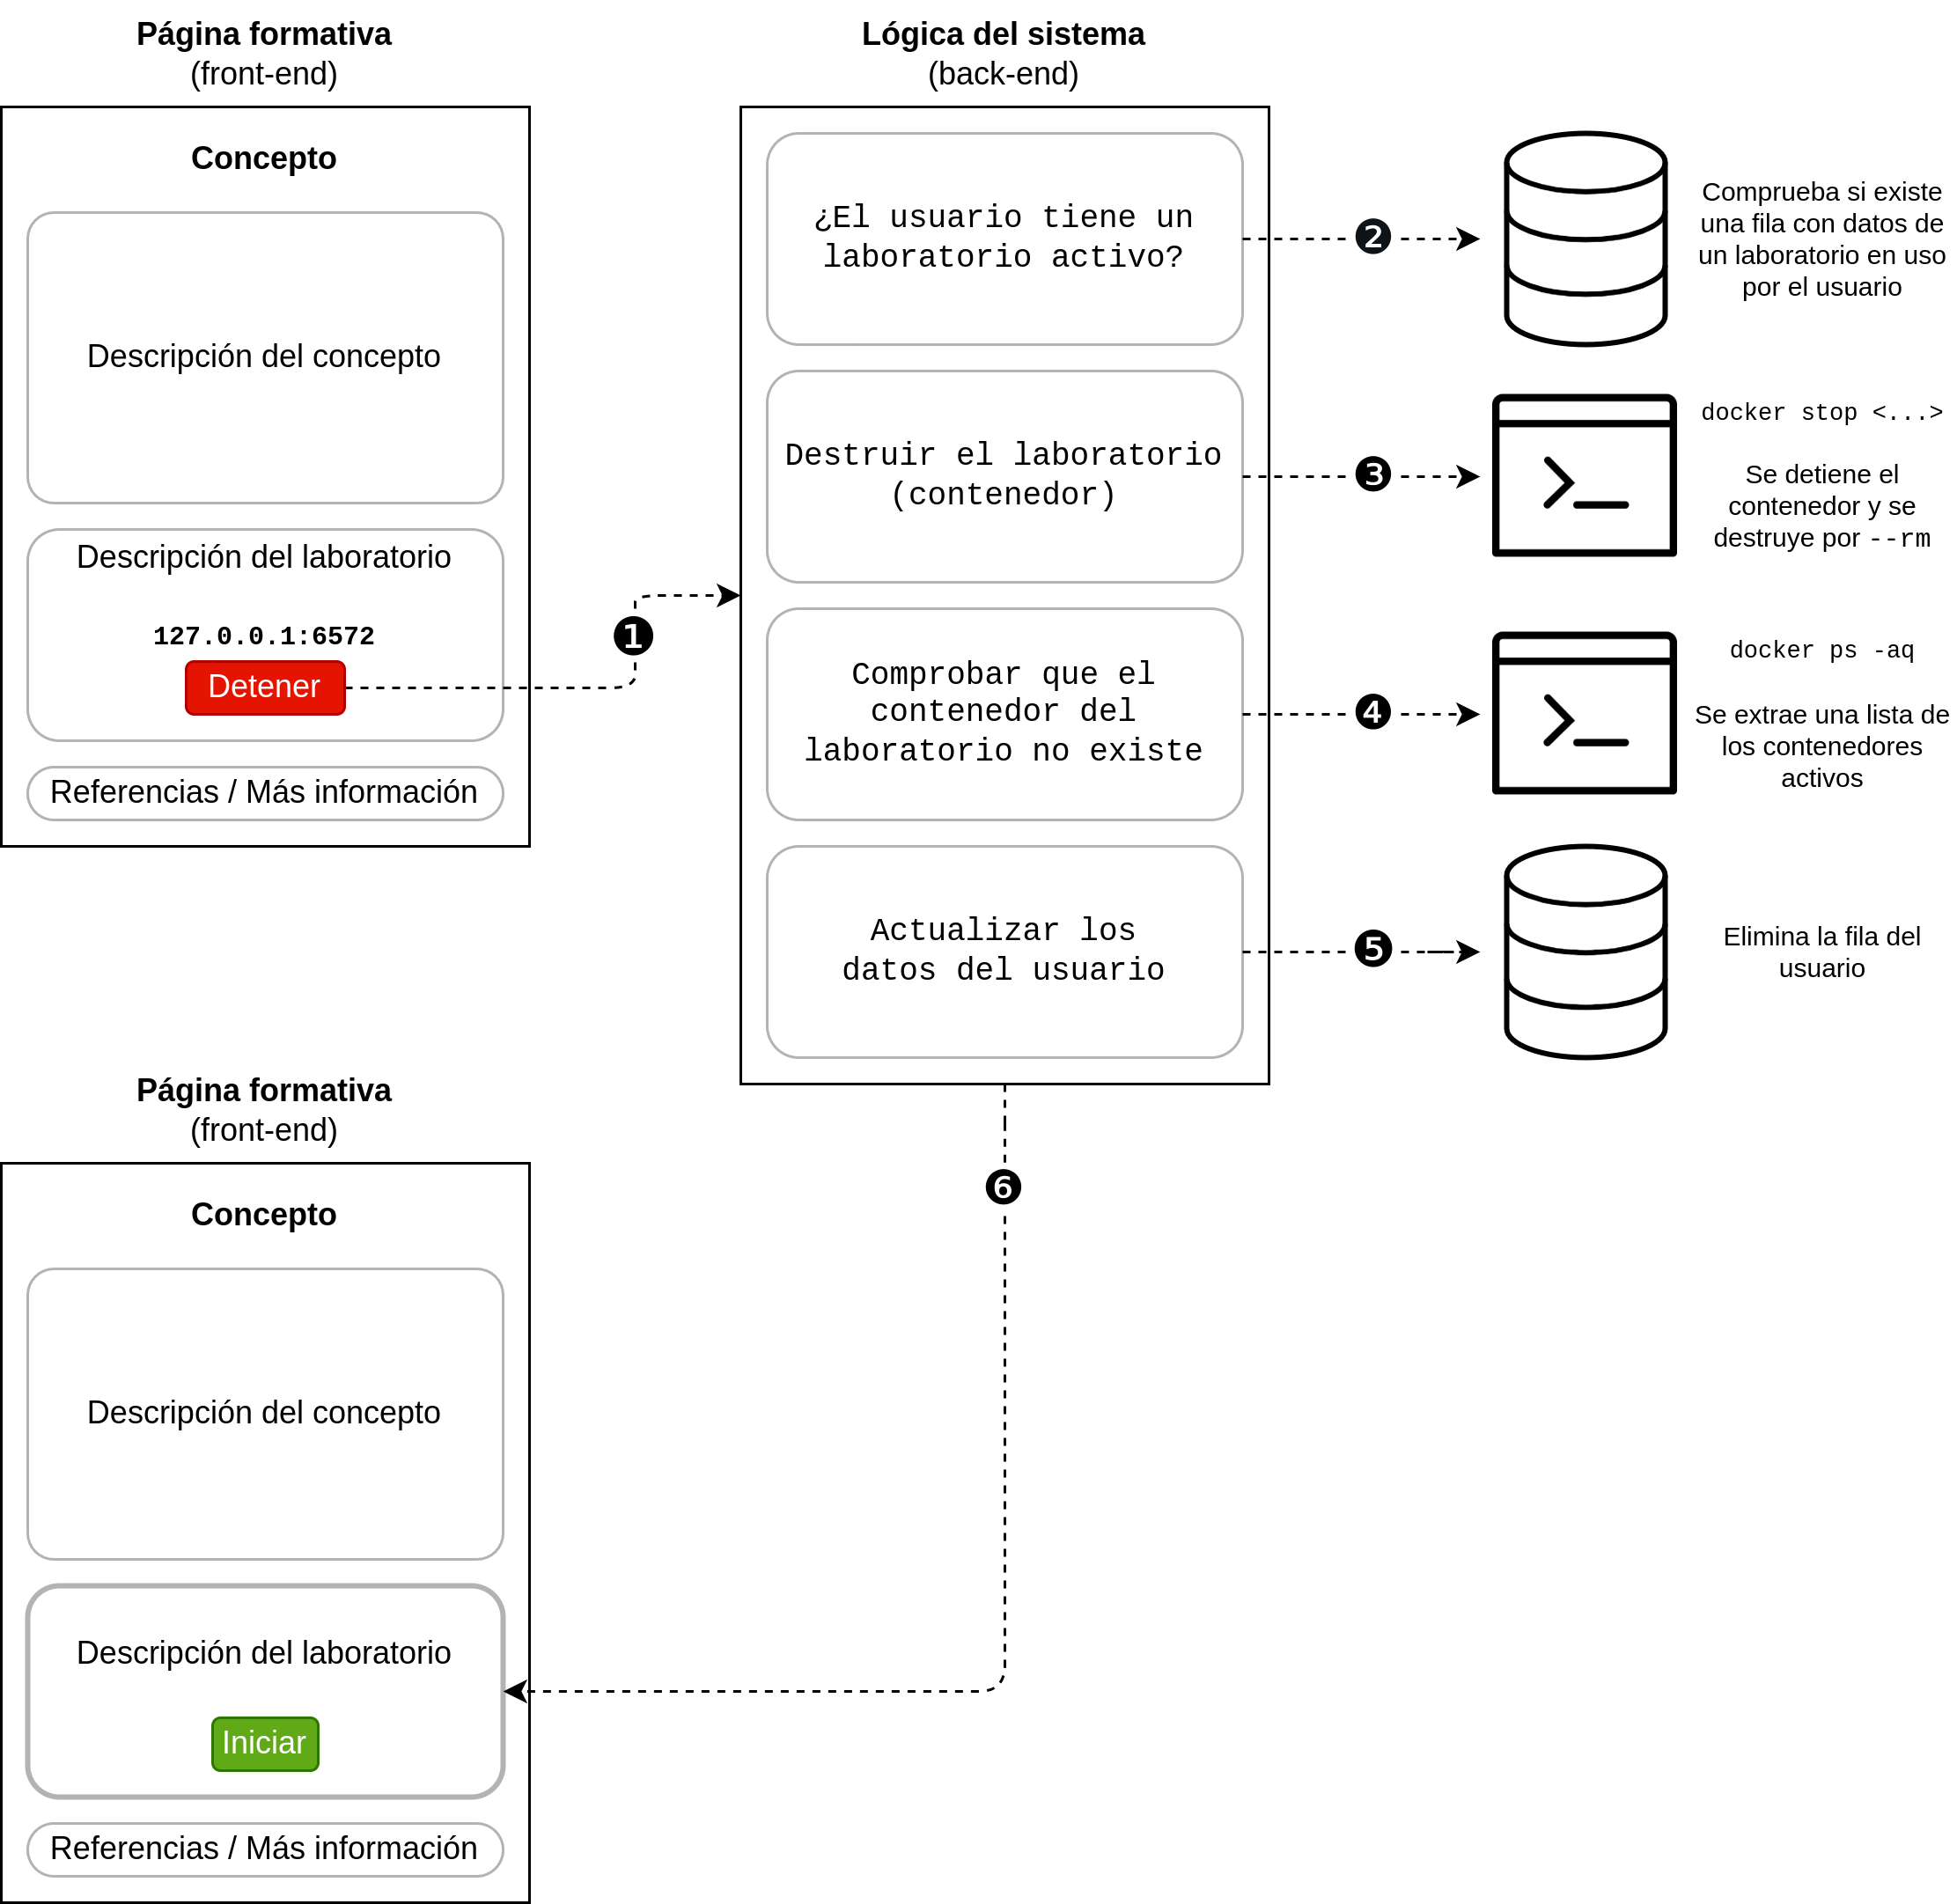
\includegraphics[scale=0.125]{images/Diagramas/detener.png}
                \caption{Destrucción de un laboratorio desde el sitio web}
                    \label{fig:detener-laboratorio}
            \end{figure}

            Este diagrama representa un uso normal de la plataforma, donde el usuario accede a la página web y desea detener el laboratorio activo.

            Se detallan a continuación los pasos que se llevan a cabo:

            \begin{enumerate}
                \item El usuario solicita detener el laboratorio activo porque ha terminado de usarlo (o quiere usar otro) pulsando el botón de detener, ejecutando algunas de las funcionalidades de la plataforma definidas en \texttt{functions.php}.

                \item Se comprueba en la base de datos que el usuario activo tiene un laboratorio activo y se obtienen los datos del mismo.

                \item Se hace una llamada al sistema para detener el contenedor Docker usando la ID obtenida en el paso anterior. Como todos los contenedores se han creado con la opción \texttt{--rm}, al detenerse son eliminados.

                \item Se hace una llamada al sistema para comprobar que el contenedor se ha eliminado correctamente. Se ejecuta el comando \texttt{docker ps -aq} (lista de IDs de todos los contenedores existentes) y se comprueba que no aparece el contenedor en la lista.
                
                \item Se elimina la entrada de la base de datos asociada al laboratorio activo.

                \item Se cambia el estado de la sección \textit{Laboratorio} de la página: se elimina la IP de la plataforma y el puerto del sistema asociado al contenedor y se cambia el botón de la sección para que ahora inicie de nuevo el laboratorio.
                
            \end{enumerate}

            Para facilitar la interpretación, no se han contemplado los errores que pueden ocurrir durante el proceso.

            \newpage


            \begin{figure}
                \centering

                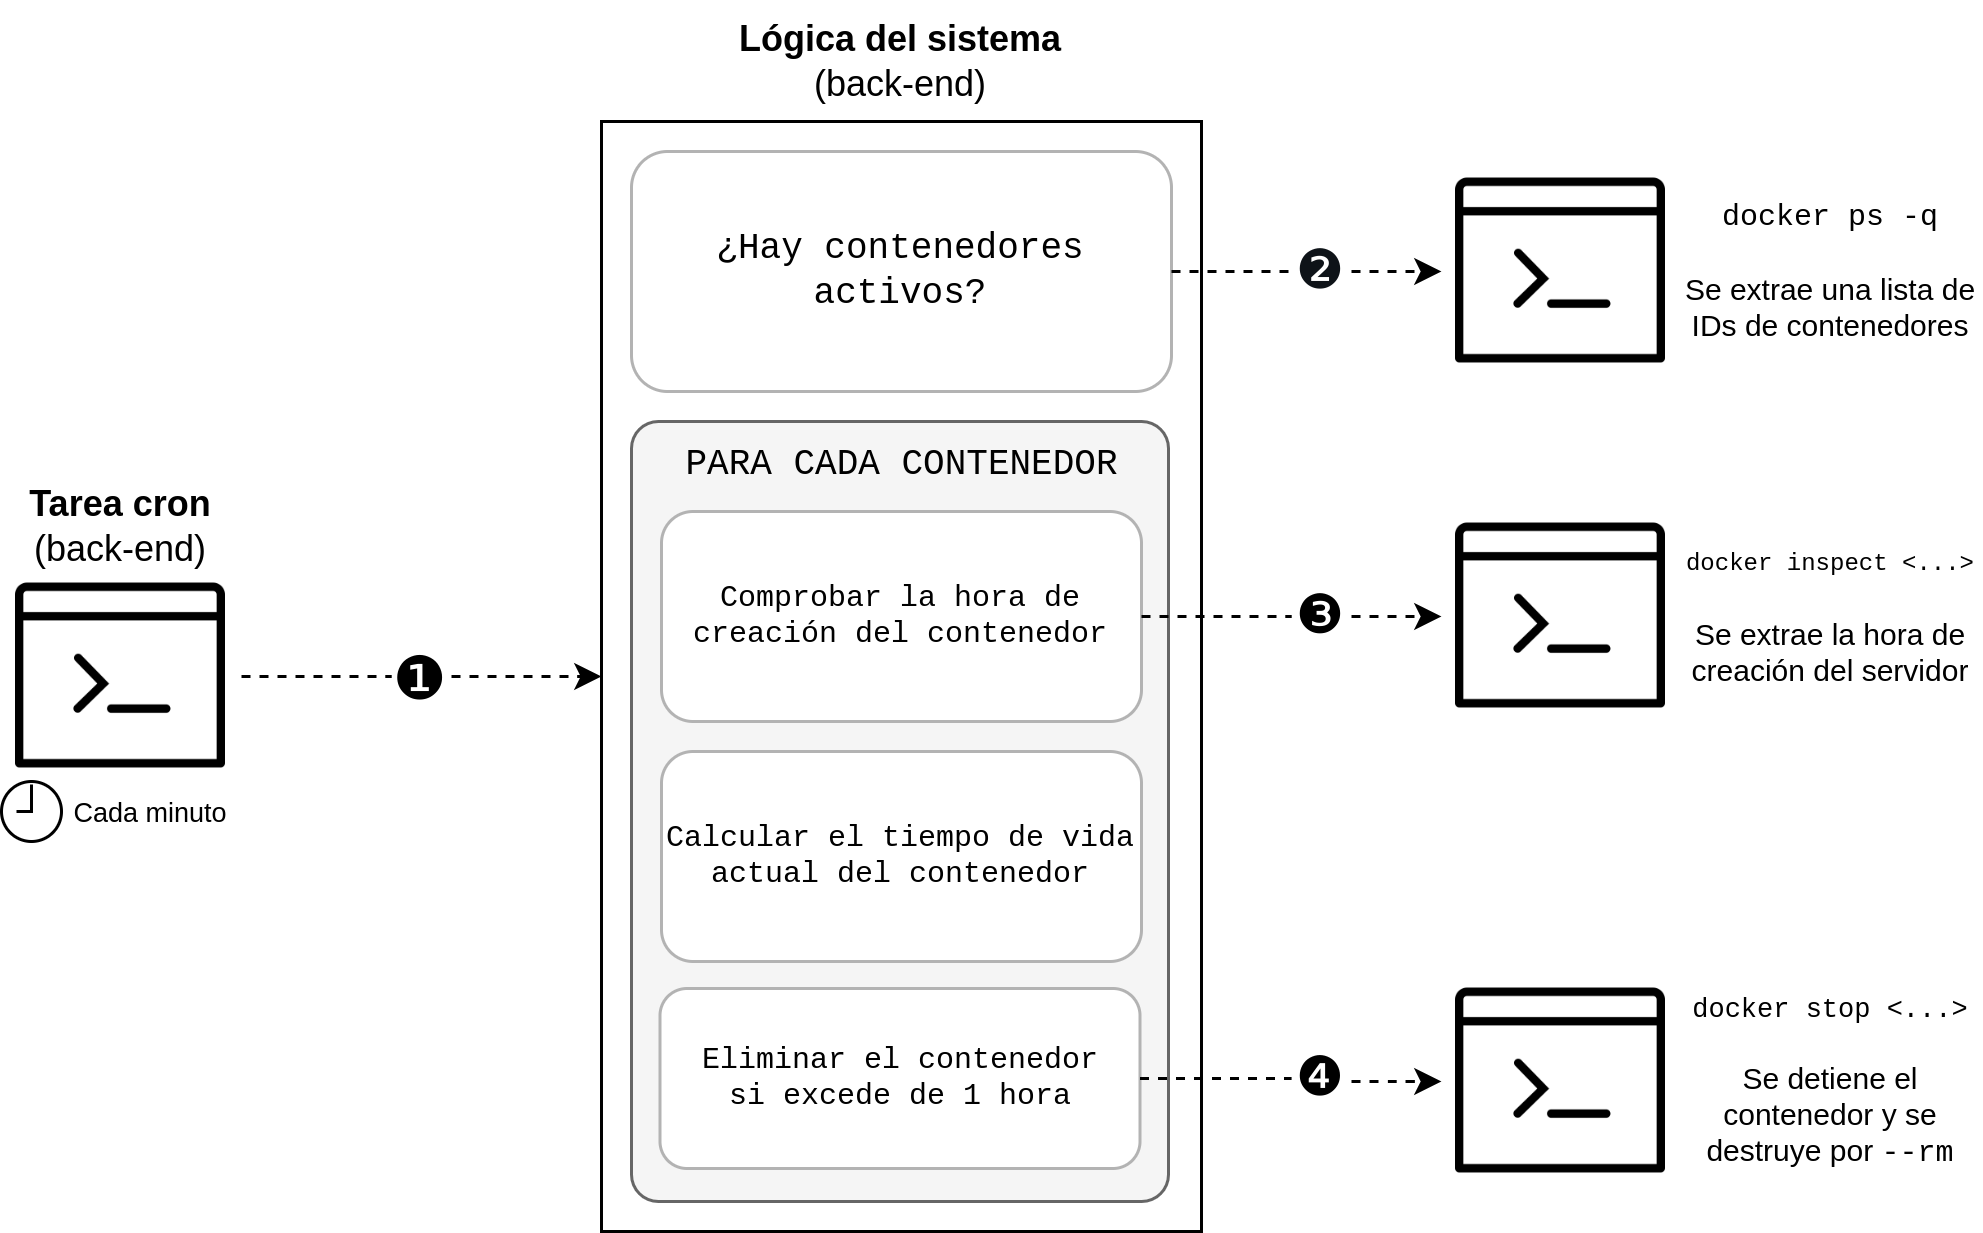
\includegraphics[scale=0.15]{images/Diagramas/detener-cron.png}
                \caption{Destrucción automática de un laboratorio}
                    \label{fig:detener-cron-laboratorio}
            \end{figure}

            Este diagrama representa un uso normal de una tarea de cron con la que detener y eliminar automáticamente laboratorios que excedan su tiempo de vida.

            Se detallan a continuación los pasos que se llevan a cabo:

            \begin{enumerate}
                \item La tarea cron del sistema ejecuta un script de Bash para detener los contenedores Docker que se encuentren activos y cuyo tiempo de vida exceda a 1 hora. Esta tarea se ejecuta cada minuto.

                \item Se hace una llamada al sistema para comprobar si hay contenedores activos y en caso afirmativo, obtener una lista de los IDs de esos contenedores; el script termina en caso de no haber ninguno.

                \item Se usa la lista en un bucle para iterar sobre ella y se hace una llamada al sistema para obtener la hora de creación del contenedor actual. Esos datos se usan para calcular el tiempo de vida del contenedor actual.
                
                \item Se comprueba si el tiempo de vida del contenedor actual excede a 1 hora y si es así, se detiene. Como los contenedores han sido creados con la opción \texttt{--rm}, al detenerse son eliminados.
            \end{enumerate}

            Este script muestra información cada vez que se ejecuta, haciendo que la tarea de cron almacene dicha información en un archivo de texto a modo de registro.

            \begin{figure}[htbp]
                \centering

                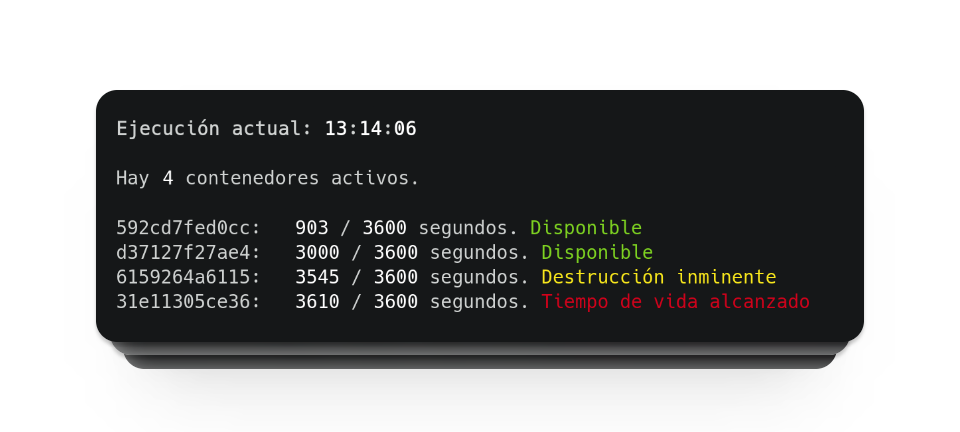
\includegraphics[scale=0.3]{images/Capturas/cron-log.png}
                \caption{Salida del script de la tarea de cron}
                    \label{fig:detener-cron-log}
            \end{figure}

            \newpage
        
        
    \section{Catálogo de conceptos}
        \label{sec:catalogo}

        A continuación se muestra una serie de conceptos que se consideran básicos para todo usuario que quiera aprender sobre pentesting. El catálogo incluye conceptos genéricos, ataques más comunes y algunos casos más específicos para que el usuario pueda tener una visión general de las posibilidades que ofrece el sector de la ciberseguridad.

        Cada concepto incluye una pequeña descripción, el motivo de inclusión al sitio web y una breve descripción de la funcionalidad de un laboratorio asociado.

        También, cabe destacar que el texto mostrado en este documento en relación a los conceptos no se corresponde con la versión final -más elaborada y detallada- del sitio web del proyecto, ya que está orientado a la memoria y no al usuario final.

        \subsection{Introducción básica a Linux y Bash scripting}
            \label{sec:catalogo-linux-bash}

            Linux es un sistema operativo de código abierto basado en UNIX creado en 1991, y aunque inicialmente fue desarrollado para ordenadores personales, actualmente se utiliza en una gran variedad de dispositivos (servidores, dispositivos móviles, sistemas embebidos...).

            Por otro lado, Bash es un lenguaje de scripting que se ejecuta en la terminal de Linux, y que permite automatizar tareas de forma sencilla.

            Este proyecto está orientado a aquellos usuarios que quieren empezar en el sector de la ciberseguridad, por lo que se ha considerado adecuado incluir una breve introducción tanto para Linux como para scripting con Bash: la primera, porque resulta evidente el abundante uso de sistemas operativos basados en Linux en el sector; y la segunda, porque es el lenguaje de scripting más utilizado en dichos sistemas operativos.

            \begin{tabular}{|m{0.45\linewidth}|m{0.45\linewidth}|}                
                \hline
                \textbf{Linux} & \textbf{Bash} \\
                \hline
                Estructura y función de los directorios & Ejecución de comandos \\
                Permisos de archivos y directorios & Variables \\
                Gestión de procesos & Estructuras de control \\
                Gestión de usuarios y grupos & Funciones \\
                Gestión de paquetes & Expresiones regulares \\
                Gestión de servicios & \\
                \hline
            \end{tabular}

            \paragraph{Laboratorio}

                Un entorno virtualizado que usara un sistema operativo basado en UNIX donde el usuario pudiera revisar y manipular su contenido, así como ejecutar comandos de Bash.

                Este entorno podría ser útil para aquellos usuarios que no dispongan de un sistema operativo basado en UNIX, o que no quieran modificar el suyo para realizar pruebas.

                Se podrían plantear las siguientes opciones:
                
                \begin{itemize}
                    \item Una serie de ficheros preparados para que el usuario comprobara el funcionamiento de los permisos y pudiera modificarlos.
                    \item Solicitar al usuario datos e información del sistema operativo extraíbles mediante comandos de Bash.
                    \item Incluir scripts de prueba que realizaran distintas funciones y que mostraran los distintos aspectos del lenguaje.
                \end{itemize}


        \subsection{OSINT y Esteganografía}

            La inteligencia de código abierto (\textit{Open Source INTelligence}) es una técnica de investigación que se basa en la obtención de información a partir de fuentes de acceso público. Esta técnica se utiliza en el sector de la ciberseguridad para obtener información sobre un objetivo, como puede ser una persona, una empresa o una organización, con el objetivo de realizar un ataque posterior.

            La esteganografía es una técnica de ocultación de información dentro de un archivo, como puede ser una imagen, un vídeo o un archivo de audio. Esta técnica se utiliza en el sector de la ciberseguridad para ocultar información sensible dentro de archivos que no levanten sospechas, como puede ser una imagen de perfil de una red social, un vídeo de YouTube o un archivo de audio de Spotify.

            Ambas técnicas suelen ir de la mano y son bastante comunes aplicarlas en situaciones reales, por lo que se ha considerado adecuado incluir las para que el usuario pueda familiarizarse con ellas.
                
            \paragraph{Laboratorio}

                Un entorno virtualizado que incluyera una serie de archivos con información oculta que el usuario pudiera extraer mediante distintas herramientas de esteganografía.

                Previamente, se mostraría en la sección teórica algunas herramientas online y de escritorio que permiten extraer información oculta de archivos.

                Se podrían plantear las siguientes opciones:
                
                \begin{itemize}
                    \item Ocultar información en distintos archivos, haciendo que el usuario ponga en práctica lo aprendido acerca de técnicas y herramientas de OSINT junto a esteganografía.
                \end{itemize}

            
            \subsection{Hash-cracking y Fuerza Bruta}

                El hash-cracking es una técnica de ataque que se utiliza para obtener la contraseña original a partir de un hash.

                La fuerza bruta es una técnica de hacking en la que se intenta adivinar una contraseña o credencial de acceso probando diferentes combinaciones hasta encontrar la correcta.
                
                Estos ataques suelen ser automatizados y pueden ser extremadamente efectivos si el atacante tiene suficiente tiempo y recursos. No obstante, ambas técnicas son utilizadas con frecuencia en los tests de intrusión para comprobar la seguridad y robustez de una contraseña.

                Estos conceptos del catálogo van de la mano con los siguientes, pero se ha considerado adecuado separarlos porque estos se centran más en la obtención de contraseñas, mientras que los siguientes se centran justo en lo contrario, en la creación de contraseñas robustas. 

                \paragraph{Laboratorio}

                    Un entorno virtualizado que incluyera una serie de hashes con distintos algoritmos y diccionarios de contraseñas.

                    Se podrían plantear las siguientes opciones:
                    
                    \begin{itemize}
                        \item Incluir usuarios en el sistema con contraseñas conocidas y solicitar al usuario obtenerlas con fuerza bruta usando diccionarios de contraseñas.
                        \item Incluir diversos hashes de algoritmos disintos y solicitar al usuario obtener las contraseñas originales mediante hash-cracking.
                    \end{itemize}


            \subsection{Criptografía y Cifrado}

                La criptografía es una técnica que se utiliza para cifrar y descifrar información, cuyo objetivo es que solo el emisor y el receptor puedan acceder a ella.

                El cifrado es una técnica que se utiliza para codificar información, con el objetivo de que solo el emisor y el receptor puedan acceder a ella.

                Ambas técnicas son utilizadas con frecuencia en los tests de intrusión para comprobar la seguridad y robustez de una contraseña.

                Estos conceptos del catálogo van de la mano con los anteriores, pero se ha considerado adecuado separarlos porque estos se centran más en la creación de contraseñas robustas, mientras que los anteriores se centran justo en lo contrario, en la obtención de contraseñas. 

                \paragraph{Laboratorio}

                    Un entorno virtualizado que incluyera una serie de archivos cifrados y que el usuario pudiera descifrar mediante distintas herramientas de criptografía y cifrado.

                    Se podrían plantear las siguientes opciones:
                    
                    \begin{itemize}
                        \item Incluir archivos cifrados con distintos algoritmos y solicitar al usuario descifrarlos mediante distintas herramientas de criptografía.
                        \item Incluir archivos cifrados con distintos algoritmos y solicitar al usuario descifrarlos mediante distintas herramientas de cifrado.
                    \end{itemize}

        
        \subsection{Escalada de privilegios en Linux}

            La escalada de privilegios es una técnica de hacking que se utiliza para obtener acceso a sistemas o recursos que normalmente estarían restringidos por permisos de seguridad. Esta técnica se utiliza cuando un atacante ya ha obtenido acceso a un sistema con un conjunto limitado de permisos, pero necesita obtener permisos adicionales para llevar a cabo acciones malintencionadas.
                
            En este tipo de ataque, el atacante busca explotar vulnerabilidades en el sistema operativo o en las aplicaciones instaladas para obtener permisos de administrador o de otro usuario privilegiado. Una vez que se obtienen estos permisos, el atacante puede tener acceso a información confidencial, instalar malware o tomar el control total del sistema.

            \paragraph{Laboratorio}

                Un entorno virtualizado que incluyera un sistema Linux con vulnerabilidades de escalada de privilegios registradas y replicables usando GTFOBins.

                Se podrían plantear las siguientes opciones:
                
                \begin{itemize}
                    \item Ganar acceso a una shell root usando \texttt{find}.
                    \item Ganar acceso a una shell root usando \texttt{sudo}.
                    \item Ganar acceso a una shell root usando una tarea de cron.
                \end{itemize}

        
        \subsection{Introducción a Redes y Protocolos}

            Una red de ordenadores es un conjunto de dispositivos electrónicos conectados entre sí a través de un medio, que intercambian información y comparten recursos.
            
            Los protocolos de red definen un conjunto de reglas y convenciones para lelvar a cabo la comunicación entre dispositivos en una red. Los protocolos de red incluyen mecanismos para la autenticación, la transferencia de datos, la detección de errores y la corrección de errores, y la señalización.

            Al igual que pasó con la sección \textit{Introducción básica a Linux y Bash scripting} \ref{sec:catalogo-linux-bash}, esta podría consistir en una introducción a conceptos relevantes sobre este campo, ya que será más útil en el resto de componenentes del catálogo.

            
        \subsection{Análisis de tráfico}
            
            Esta es una técnica de ciberseguridad que implica la monitorización y el examen de los datos que fluyen a través de una red de comunicaciones; puede incluir la recopilación de información sobre el origen y el destino de los datos, el tipo de protocolo utilizado, la cantidad de datos transmitidos y otros metadatos relacionados con el tráfico... y puede ser utilizado para detectar patrones de actividad sospechosa en una red, como la transferencia de grandes cantidades de datos o la comunicación con direcciones IP o puertos inusuales. También puede ser utilizado para identificar amenazas específicas, como ataques de denegación de servicio o intentos de acceso no autorizado a sistemas.
            
            El análisis de tráfico puede llevarse a cabo utilizando herramientas de software especializadas que pueden recopilar y analizar los datos de la red en tiempo real. Estas herramientas pueden generar alertas automáticas cuando se detecta actividad sospechosa y proporcionar informes detallados sobre el tráfico de red.
            
            Cabe resaltar que el análisis de tráfico puede presentar desafíos legales y de privacidad, ya que puede involucrar la monitorización de datos confidenciales, por lo que es importante asegurarse de que cualquier análisis de tráfico se lleve a cabo de manera legal y ética y que se respeten las políticas de privacidad y seguridad de la organización.

            \paragraph{Laboratorio}

                Un entorno virtualizado que incluyera algunas herramientas con las que generar tráfico de red, para que el usuario pueda conectarse a él e intercambiar tráfico usando su propio entorno virtualizado o

                Se podrían plantear las siguientes opciones:

                \begin{itemize}
                    \item Incluir \texttt{ftp} para que el usuario pueda ver el tráfico -en texto claro- generado al transferir archivos.
                \end{itemize}


        \subsection{Conceptos a revisar}

            \subsubsection{Escaneo de puertos y enumeración de servicios}
        
                El escaneo de puertos es una técnica donde se envían paquetes a un rango de puertos de un sistema con el objetivo de encontrar aquellos que están abiertos y escuchando conexiones; esta técnica se utiliza para descubrir posibles vulnerabilidades en sistemas informáticos y redes.
                
                La enumeración de servicios, por otro lado, es el proceso de identificación y catalogación de los servicios que se están ejecutando en un sistema informático. Los servicios son programas que se ejecutan en segundo plano en un sistema informático y que se utilizan para proporcionar una funcionalidad específica.
                
                
            \subsubsection{Inyección SQL}
                
                La inyección SQL es una técnica de ataque que se utiliza para explotar vulnerabilidades en las aplicaciones web que interactúan con bases de datos. Esta técnica se basa en la inserción de código SQL malintencionado en los campos de entrada de una aplicación, con el fin de obtener acceso no autorizado a los datos almacenados en la base de datos o incluso tomar el control del servidor.
                
                La inyección SQL se aprovecha de la falta de validación o sanitización de los datos de entrada que son utilizados en las consultas SQL. Cuando los datos de entrada no son validados correctamente, los atacantes pueden introducir código SQL malintencionado que es ejecutado por la aplicación. Esto puede permitir a los atacantes extraer información confidencial, realizar modificaciones en la base de datos o incluso tomar el control total del servidor.
            
            
            \subsubsection{Ataques de \textit{buffer overflow}}
                
                Un ataque de \textit{buffer overflow} es una técnica de explotación de vulnerabilidades en la memoria de un programa que permite a un atacante ejecutar código malicioso en un sistema. El ataque se produce cuando un programa intenta escribir datos en un buffer de memoria, pero la cantidad de datos escritos excede la capacidad del buffer, permitiendo al atacante escribir un bloque de código malicioso en el buffer y sobreescribir la dirección de retorno de la función, para que apunte al código malicioso en lugar de volver a la función llamada originalmente.
                
                Este tipo de ataque puede ser especialmente peligroso si el programa original que se está ejecutando tiene privilegios elevados, ya que el código malicioso puede ejecutarse con esos mismos privilegios. Por lo tanto, los ataques de \textit{buffer overflow} pueden ser utilizados para obtener acceso no autorizado a un sistema o para ejecutar código malicioso en un sistema.


        \subsection{Conceptos extra}

            Estos elementos del catálogo son algo más específicos, pero se han incluido porque son conceptos que se suelen encontrar en el mundo de la ciberseguridad y que pueden ser interesantes de conocer.

            \subsubsection{Bypass}

                Esta técnica se utiliza para evitar un mecanismo de seguridad o restricción, y puede ser utilizada por atacantes para eludir las medidas de seguridad de un sistema o para evadir las restricciones de acceso a los recursos de un sistema.

                \paragraph{Laboratorio}

                    Un entorno virtualizado que incluyera un sistema con algún tipo de restricción de acceso a un recurso, para que el usuario pudiera intentar eludir dicha restricción.

                    \begin{itemize}
                        \item Un servidor de Git con la vulnerabilidad CVE-2017-8386.
                    \end{itemize}


            \subsubsection{Ransomware}
            
                El ransomware es un tipo de malware que se utiliza para cifrar los archivos de un sistema informático y exigir un rescate a cambio de la clave de descifrado. Este tipo de malware se propaga a través de archivos adjuntos de correo electrónico, sitios web maliciosos o a través de vulnerabilidades en el sistema operativo o las aplicaciones instaladas.
                
                El ransomware puede ser especialmente peligroso porque puede cifrar los archivos de un sistema informático y exigir un rescate a cambio de la clave de descifrado. Esto puede causar graves daños a las organizaciones, ya que puede provocar la pérdida de datos importantes o incluso la interrupción de las operaciones comerciales.

                Esta sección pretende enseñar al usuario lo sencillo que es desarrollar un ransomware al mismo tiempo que se muestra lo verdaderamente peligroso que puede llegar a ser.
                
                \paragraph{Laboratorio}
                
                    Un entorno virtualizado con un ransomware ejecutable por el usuario.
            
            \cleardoublepage


\chapter{Problemas encontrados}

        Esta sección tratará distintas problemáticas que se han abordado durante el desarrollo del proyecto, de forma que se puedan entender mejor las decisiones tomadas y redactadas en los capítulos anteriores de esta memoria.

        No se incluyen aquellos problemas que se hayan resuelto con investigación, como por ejemplo: saber usar algunas funcionalidades de WordPress, qué casos incluir en los laboratorios, etc.

    \section{Gestión local de contenedores Docker}

        Durante todo el documento se ha hablado de la funcionalidad del proyecto: una plataforma web que permite a los usuarios acceder a laboratorios virtuales donde poner en práctica los conocimientos adquiridos en la propia plataforma, siendo dichos laboratorios contenedores Docker que el usuario puede iniciar o detener a voluntad desde el sitio web, aunque con ciertas limitaciones.
        
        Sin embargo, esto planteaba un problema: cómo se podrían gestionar esos contenedores Docker. 

        \subsubsection{Conexión entre el sitio web y Docker}

            El objetivo se trataba de algo tan simple como levantar y destruir contenedores Docker, sin embargo, esto debía hacerse de forma dinámica, ya que el resultado final esperado era tener un sistema donde los contenedores no estuvieran permanentemente activos, sino que fueran activados y desactivados en función de su uso.
            
            El uso de estrategias como Kubernetes excedían a las propias necesidades del proyecto, ya que al tratarse de una prueba de concepto no se requería gestionar un gran número de contenedores, ni tampoco era necesario que se organizaran en clústeres; por tanto, se decidió que los contenedores se gestionarían de forma local.
            \begin{figure}[htbp]
                \centering

                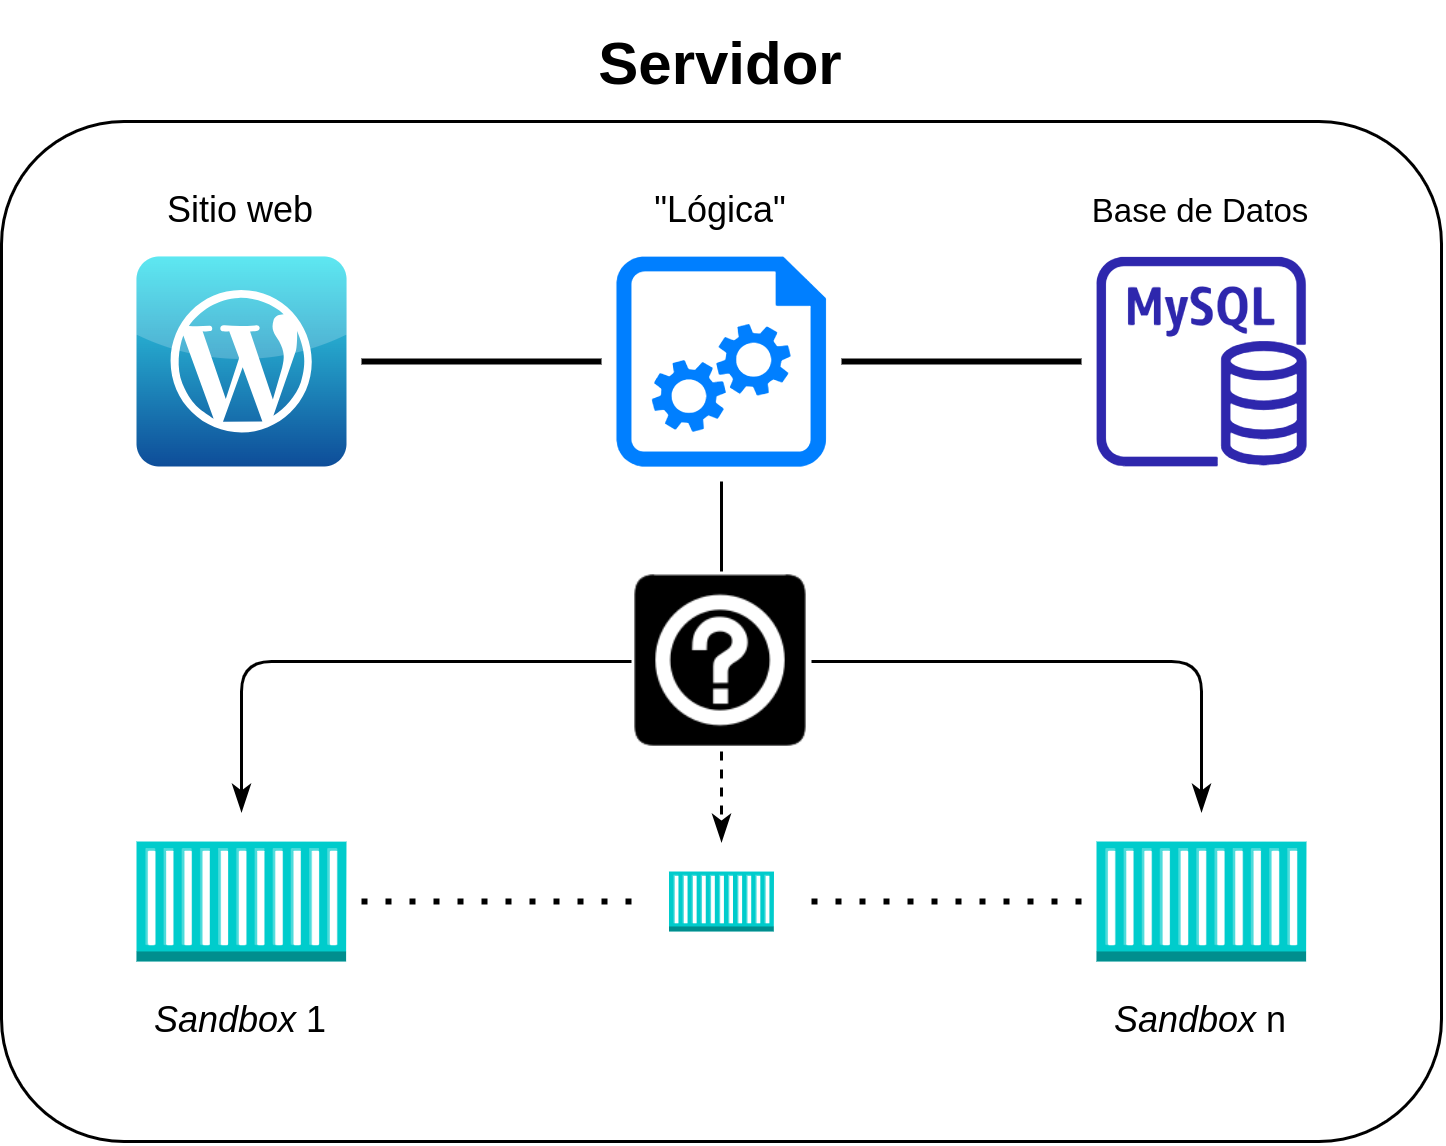
\includegraphics[width=0.5\textwidth]{images/Diagramas/conexion.png}
                \caption{Representación gráfica del problema de conexión entre el sitio y los contenedores}
                \label{fig:conexion}
            \end{figure}

            Tampoco se usaron APIs ni librerías, ya que se consideró que no era necesario, y que se podía hacer uso de los propios comandos del sistema para gestionar los contenedores Docker; de nuevo, porque la idea en sí resultaba muy simple, aunque más tarde su complejidad fue creciendo.

            El resultado final fue el uso del siguiente comando del sistema, que se ejecuta usando \texttt{shell\_exec()} en el fichero \texttt{functions.php} del sitio web:
            
            $$
            \texttt{docker run --rm -p \${puerto}/22 -d \${laboratorio}:latest}
            $$
            
            El comando recibe un puerto libre del sistema y el nombre del laboratorio (imagen Docker) para crear el contenedor, indicado como variables PHP en la instrucción anterior. La opción \texttt{--rm} se usa para que el contenedor se destruya automáticamente al detenerse, y la opción \texttt{-d} para que se ejecute en segundo plano (aún en segundo plano devolverá la ID del contenedor creado).


        \subsubsection{Mapeo de puertos si solapamientos}

            Por otro lado, se presentaba el siguiente problema, ¿cómo se podría gestionar el mapeo de puertos de los contenedores Docker de forma automática?

            Al no usar Kubernetes, no se podía usar el mapeo de puertos de forma dinámica, ya que los contenedores se gestionaban de forma local y no se podía acceder a ellos desde fuera de la máquina donde se ejecutaban, por lo que se decidió que los contenedores se gestionarían de forma local.

            \begin{figure}[htbp]
                \centering

                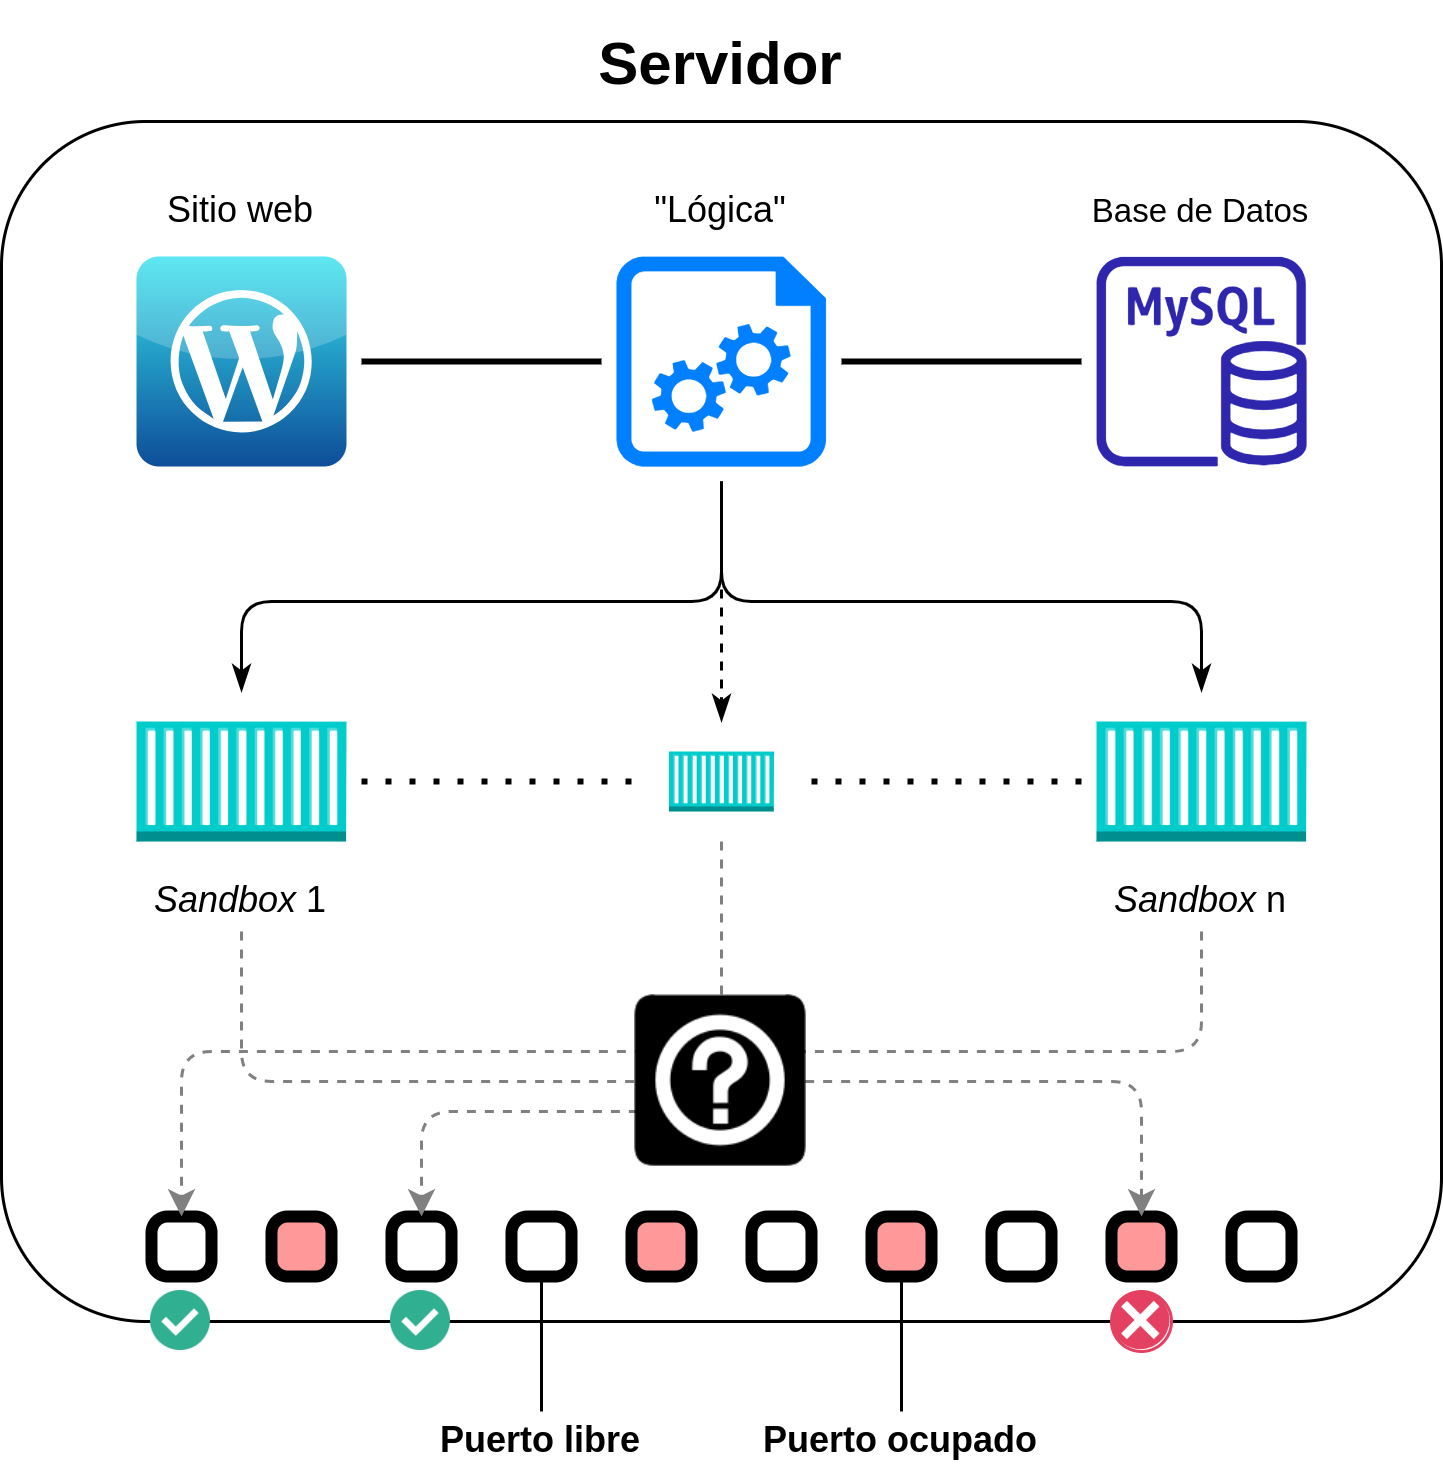
\includegraphics[width=0.5\textwidth]{images/Diagramas/puertos.png}
                \caption{Representación gráfica del problema de mapeo de puertos}
                \label{fig:mapeo-puertos}
            \end{figure}

            La opción \texttt{-p} de Docker permite mapear puertos de forma estática, lo que implica que si se usaba un puerto que ya estuviera en uso, la creación del contenedor fallaría.
            
            Por otra parte, es posible usar un rango de puertos con esa opción, lo que permite a Docker mapear un puerto del contenedor a cualquier puerto libre en el rango específicado de forma automática y aleatoria (la selección no es secuencial); esta parecería la opción perfecta pero tenía una gran limitación: los puertos libres de un rango de puertos solo son conocidos entre los contenedores de la misma imagen, y por tanto, como cada laboratorio es una imagen Docker de la que se construyen contenedores para los usuarios, esto quiere decir que no era posible determinar todos los puertos libres para todas las imágenes.
            
            Otra opción que se contempló fue la de usar el mismo rango para todas las imágenes, pero uno tan amplio que se redujera todo lo posible la posibilidad de colisiones de puertos entre contenedores de distintas imágenes; sin embargo, esta opción fue descartada porque, aunque pudiera haber sido efectiva en esta prueba de concepto, no dejaba de existir la posibilidad de que se produjeran colisiones, y por tanto, no se consideró una solución aceptable.

            El uso de ficheros \texttt{docker-compose.yml} también era muy restrictivo, ya que no permitía la gestión dinámica de puertos; para ser más específicos, este fichero almacena una configuración a la que se puede llegar usando combinaciones de opciones y valores de comandos Docker, por lo que no añade ninguna funcionalidad adicional, sino que solo permite almacenar una configuración. Aquí se reptite exactamente el mismo problema de las colisiones descrito en el párrafo anterior.

            Finalmente, se optó por generar puertos disponibles usando código en \texttt{functions.php}: se define un rango inicial \texttt{(5555 - 9999)} predefinido y para cada laboratorio que quiere iniciar un usuario, se busca en la base de datos qué puertos están siendo ocupados por otros laboratorios, se calcula la diferencia entre el rango inicial y los puertos ocupados, y se selecciona un puerto aleatorio dentro de ese rango.

            Como el puerto obtenido se usa para el laboratorio, al almacenarse esa información en la base de datos, el puerto queda registrado; del mismo modo cuando el usuario o la tarea de cron destruyan un laboratorio, los datos serán liberados de la base de datos y el puerto volverá a estar disponible para su uso.


    \section{Limitaciones del uso de contenedores y Docker}
        
        Cuando una persona piensa en la ciberseguridad, se imagina la clásica imagen de un hacker tecleando comandos en una pantalla llena de terminales, pero lo cierto es que aunque muchas herramientas se usan como scripts o comandos, no todas son así y algunas requieren una interfaz gráfica para su uso.

        Sin embargo, ocurre que para este caso concreto, no podrían usarse contenedores para aplicaciones que se usen con GUI. Los contenedores pueden llegar a ejecutar aplicaciones gráficas, pero esto implicaría que los usuarios descargaran la imagen y ellos crearan los contenedores, porque si no, estarían abriendo la aplicación en el servidor, donde no tienen acceso más allá de del acceso al contenedor por SSH.

        En algunas ocasiones es posible ejecutar una GUI a través del navegador, lo que sumado al mapeo de puertos, podría permitir que el usuario accediera a la aplicación, pero esto no es posible en todos los casos y además, no es una solución que se pueda aplicar de forma genérica.
        
        Por otra parte, existe la limitación actual de solo abrir y mapear un puerto por contenedor, teniendo que tomar la decisión sobre qué hacer en cada caso o qué finalidad tiene el laboratorio: entorno virtualizado con herramientas preinstaladas y casos de uso para dichas herramientas, o contenedor vulnerable con el que trabajar desde una máquina virtual propia del usuario.


    \section{Procesos bajo el usuario \texttt{www-data}}

        Al no usar una herramienta externa como Kubernetes, todos los procesos se realizan de forma local, por lo que el usuario que ejecuta los comandos es el usuario que ejecuta el servidor web, en este caso, \texttt{www-data}.

        Esto quiere decir que para que el proyecto funcione, el usuario \texttt{www-data} debe ser el que inicie el servicio de Docker, por lo que debe tener permisos para ello.

        \begin{figure}[htbp]
            \centering

            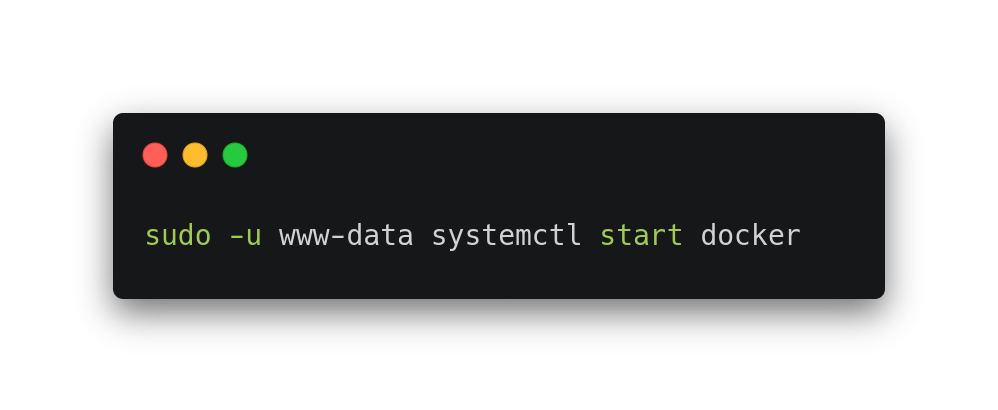
\includegraphics[width=0.75\textwidth]{images/Capturas/comandos/systemctl.png}
            \caption{Comando para iniciar el servicio de Docker como \texttt{www-data}}
            \label{fig:servicio-docker}
        \end{figure}

        Por otra parte, también necesario añadir el usuario \texttt{www-data} al grupo \texttt{docker} para que pueda ejecutar los comandos de Docker.

        \begin{figure}[!htbp]
            \centering

            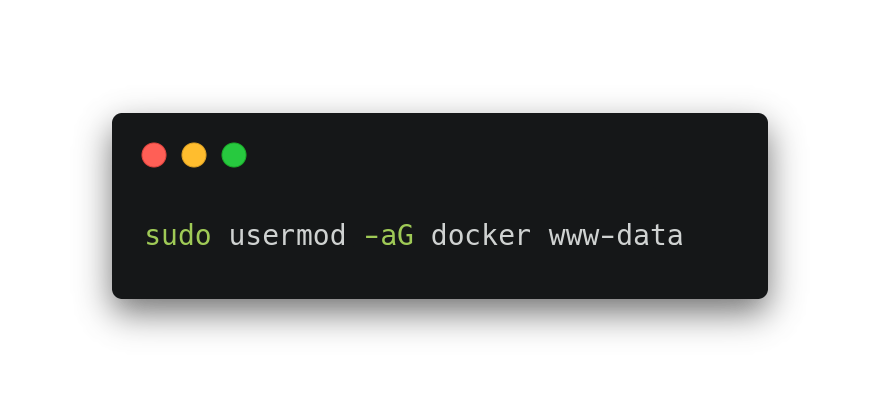
\includegraphics[width=0.75\textwidth]{images/Capturas/comandos/usermod.png}
            \caption{Cómo añadir el usuario \texttt{www-data} al grupo \texttt{docker}}
            \label{fig:usermod}
        \end{figure}

        Una vez añadido, puede comprobarse que el usuario \texttt{www-data} pertenece al grupo \texttt{docker} usando el comando \texttt{groups} o el comando \texttt{id}.

        \begin{figure}[htbp]
            \centering
            \begin{subfigure}[!htbp]{\textwidth}
                \centering

                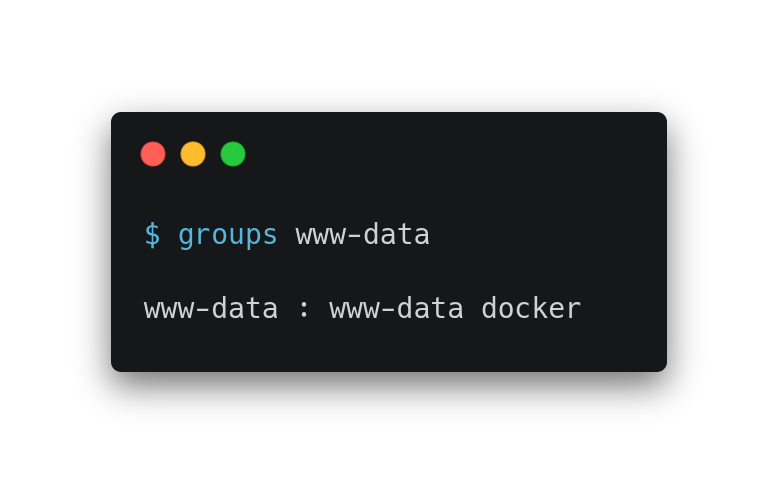
\includegraphics[width=0.75\textwidth]{images/Capturas/comandos/groups.png}
            \end{subfigure}
            \hfill
            \begin{subfigure}[!htbp]{\textwidth}
                \centering

                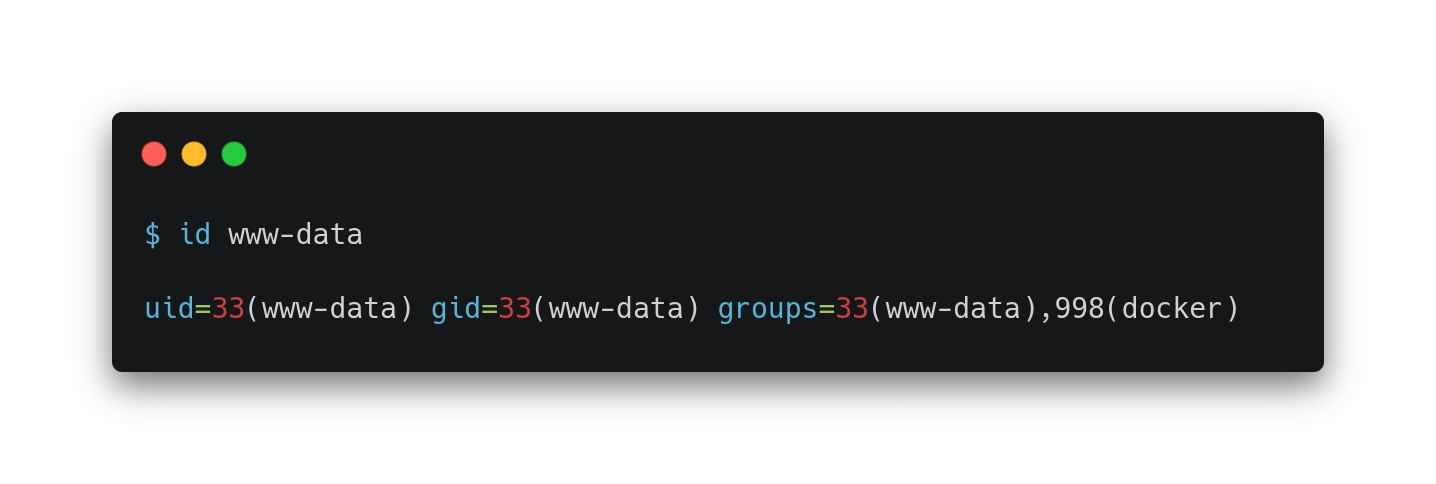
\includegraphics[width=0.75\textwidth]{images/Capturas/comandos/id.png}
            \end{subfigure}

            \caption{Comprobación de que el usuario \texttt{www-data} pertenece al grupo \texttt{docker}}
            \label{fig:grupo-docker}
        \end{figure}

        Además, del mismo modo, tendrá que crear previamente todas las imágenes de los laboratorios para que aparezcan disponibles en Docker y pueda utilizarlas: las imágenes Docker creadas por un usuario solo son visibles para ese usuario, por lo que si el usuario \texttt{www-data} no crea las imágenes, no podrá usarlas.

        Durante el desarrollo del proyecto se creó un repositorio para la creación de los laboratorios y se incluyó un script con el que actualizar las imágenes de laboratorios en el servidor, así como añadir laboratorios que no estuvieran previamente. Este script automatiza el proceso de creación de imágenes, por lo que puede ejecutarse del mismo modo que se ha mostrado con las capturas anteriores.

        \begin{figure}[!htbp]
            \centering

            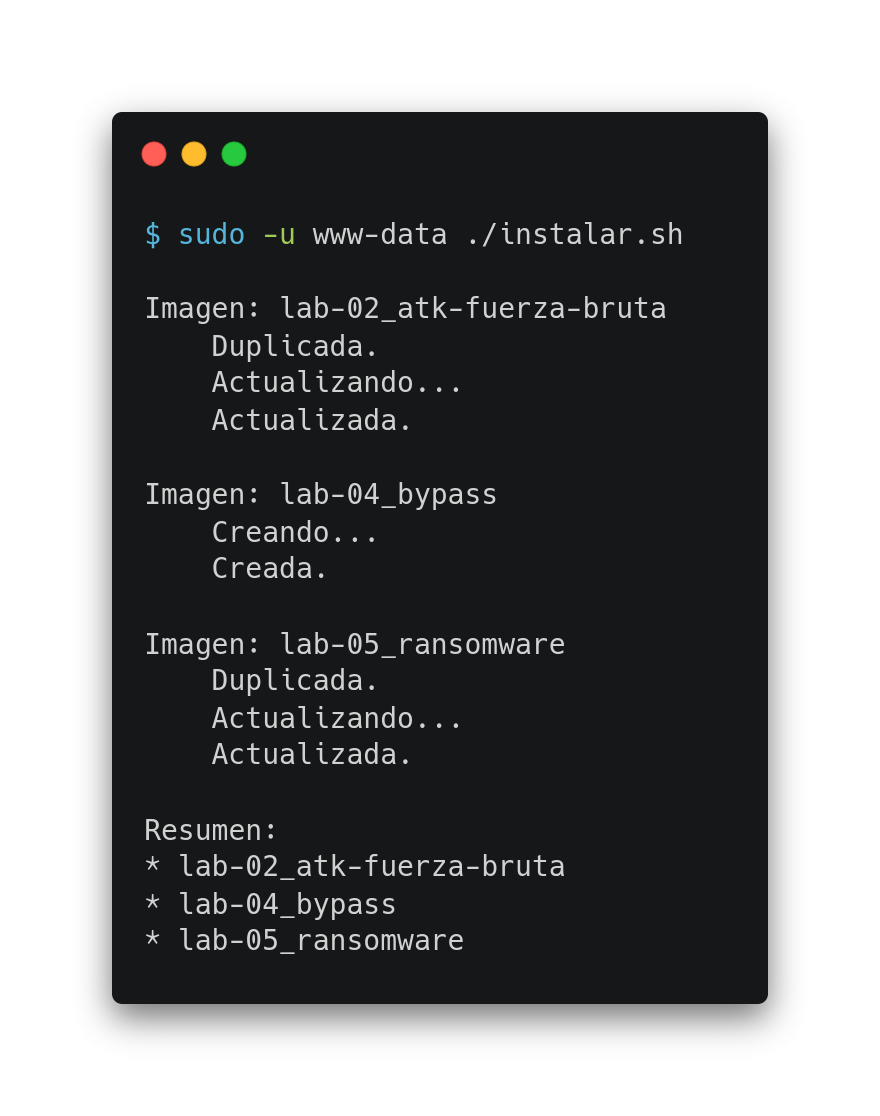
\includegraphics[width=0.5\textwidth]{images/Capturas/comandos/instalacion.png}
            \caption{Creación y actualización de las imágenes del proyecto}
            \label{fig:instalacion}
        \end{figure}

        Y por último, pasa lo mismo con la tarea de cron que automatiza la destrucción de los laboratorios: debe ser el usuario \texttt{www-data} quien defina y active la tarea de cron.

        \begin{figure}[!htbp]
            \centering

            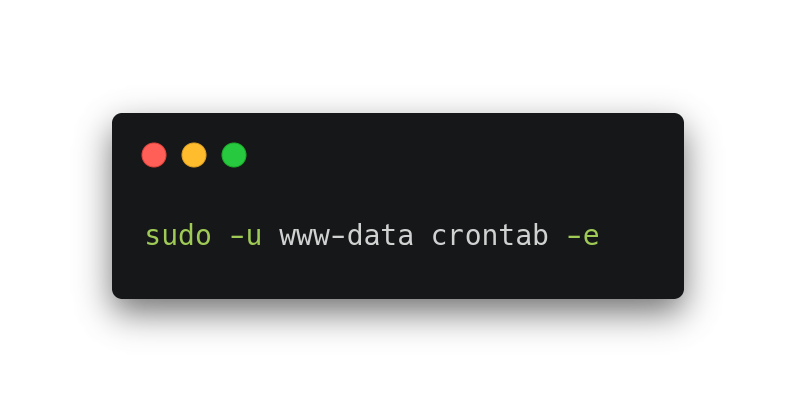
\includegraphics[width=0.5\textwidth]{images/Capturas/comandos/crontab.png}
            \caption{Comando para editar la tarea de cron como \texttt{www-data}}
            \label{fig:crontab}
        \end{figure}

        \cleardoublepage


    
\chapter{Resultados}

    \section{Cumplimiento de los requisitos}
    
    \section{Conclusiones}
    
    \section{Futuras líneas de trabajo}
        \label{sec:futuras-lineas-trabajo}
        
        Expandir el contenido de la plataforma mediante más documentación sobre conceptos adicionales, junto a nuevas pruebas virtualizadas.
        
        Elaboración de Módulos o Rutas, que se definirían como un grupo de conceptos a tratar en un orden determinado, para obtener conocimiento sobre un tema concreto.
        
        El enfoque inicial de la plataforma era el pentesting, pero si se aplicara lo anterior, podría establecerse una naturaleza genérica para abarcar muchos más conceptos de distitnas áreas de la seguridad: Administración de Sistemas, Desarrollo y Análisis de Malware... dando lugar a una plataforma más eficiente y parecida a otras ya existentes, pero manteniendo la diferencia que se fomentaba al inicio del proyecto en la sección Objetivos \ref{sec:objetivos}: una plataforma ligera, \textit{open-source} y fácilmente extensible.

        \cleardoublepage
        


\chapter{Diario}
    \label{cap:diario}

    Cada sección representa los cambios realizados hasta cada reunión.

    \section{7ª reunión: 12/04/2023}
    
        \textbf{Se crearon los capítulos: Diario \ref{cap:diario} y Borrador \ref{cap:investigacion-previa}} \\
        El primero, para incluir un historial de mi progreso; el segundo, para subir contenido WIP (\textit{work in progress}) al documento.
        
        \textbf{Se modificó el diagrama: casos de uso \ref{fig:casos-uso}} \\
        Se aplicó un estilo estándar y se mejoraron las dependencias.
        
        \textbf{Se creó la sección: Arquitectura \ref{sec:arquitectura}} \\
        Se incluyeron nuevos diagramas y contenido descriptivo sobre la arquitectura del proyecto.
        
        \textbf{Se creó la sección: Modelado de Actividades y Transacciones \ref{sec:modelado-actividades-transiciones}} \\
        Se incluyeron nuevos diagramas y contenido descriptivo de los procesos del proyecto.
        
        \textbf{Se modificó la sección: Ingeniería de Requisitos \ref{cap:ingenieria-requisitos}} \\
        Se descompusieron los requisitos anteriores en requisitos más atómicos y se han añadido nuevos requisitos no funcionales.
    
        \textbf{Se creó la sección: Estructura global del proyecto \ref{sec:estructura-global}} \\
        Se incluyó una descripción de lo que se plantea realizar con este TFG separándolo en 3 pilares fundamentales.
    
        \textbf{Se creó la sección: Proceso Creativo \ref{sec:proceso-creativo}} \\
        Se incluyó una descripción de distintos planteamientos sobre la plataforma web que tuvieron lugar durante la investigación previa del TFG. \\
        El nombre de esta sección puede variar, pero al ser un borrador, se elegió algo \textit{llamativo}.
    
        \textbf{Se inició la creación de un prototipo de la plataforma} \\
        Se está configurando una página WordPress (WIP).\\
        Se está practicando con contenedores de Docker (WIP)\\ 
        Se está tratando de levantar un contenedor a través de la página (WIP).

        \newpage


    \section{8ª reunión: 03/05/2023}

        \textbf{Se añadió una página: contraportada} \\
        Se unió el documento PDF de la contraportada del campus virtual al final del documento.

        \textbf{Se modificó la bibliografía: enlace de la ADA \cite{articulo-ada}} \\
        Se sustituyó por una versión corta y equivalente. Ahora todos los enlaces caben en la página.

        \textbf{Se modificó un diagrama: destrucción de una \textit{sandbox} \ref{fig:destruccion-laboratorio}} \\
        Se añadió un caso de control de errores y el tratamiento del tiempo de vida.

        \textbf{Se modificó una tabla: Wordpress vs Astro vs Drupal \ref{tab:wordpress-vs-astro-vs-drupal}} \\
        Se combinaron las tablas Wordpress vs Astro y Wordpress vs Drupal, de forma que aunque se mantienen sus secciones separadas (porque las comparaciones fueron distintas), solo hay una tabla como referencia.

        \textbf{Se modificó la sección: Futuras líneas de trabajo \ref{sec:futuras-lineas-trabajo}} \\
        Se reformuló el último párrafo, haciendo más hincapié en la posible expansión de la plataforma con más recursos y conceptos fuera del ámbito del pentesting, convirtiéndola no en la temática principal, sino en una de múltiples temáticas.

        \textbf{Se modificó la sección: Jupyter 5.2.2} \\
        Se estableció una conclusión para el descarte de esta tecnología en el proyecto.

        \textbf{Se modificó la sección: WordPress 1.5.2} \\
        Se añadieron nuevas referencias a la bibliografía.

        \textbf{Se creó un laboratorio: Bypass} \\
        Define el concepto de Bypass y la vulnerabilidad CVE-2017-8386 como ejemplo. \\
        El laboratorio contiene dicha vulnerabilidad para explotarla.
        
        \textbf{Se creó un laboratorio: Fuerza Bruta} \\
        Define el concepto de Fuerza Bruta, tipos de ataques más comunes y herramientas. \\
        El laboratorio contiene las herramientas \texttt{nmap} e \texttt{hydra} para que el usuario pueda obtener las credenciales del usuario administrador del entorno.
        
        \textbf{Se arregló la sección: Dependencias de contenedores Docker} \\
        La sección hacía referencia a \textit{contenedores} de Docker cuando en realidad se trataban de \textit{imágenes}. Ahora la sección cuenta con rigor y se ha optimizado el texto.

        \newpage

    \section{9ª reunión: 18/05/2023}

        \textbf{Se movió el capítulo: Borrador} \\
        El capítulo ahora es \textit{Investigación previa} (\ref{cap:investigacion-previa}).